% ============================================================================
% PROPOSAL TUGAS AKHIR (TA 1) — Program Studi Statistika UGM
% Template kelas: laporanta1mathugm.cls
% Kompilasi: latexmk -pdf skripsi_ta1.tex
% ============================================================================

\documentclass{laporanta1statugm}

% ============================================================================
% PAKET TAMBAHAN
% ============================================================================

\usepackage{bm}                     % Simbol matematika tebal
\usepackage{booktabs}               % Tabel: \toprule, \midrule, \bottomrule
\usepackage[most]{tcolorbox}        % Kotak dan kartu informasi
\usepackage{tikz}                   % Diagram dan ilustrasi
\usepackage{amsmath}                % Persamaan matematika
\usepackage{amssymb}                % Simbol matematika tambahan

\usetikzlibrary{
    shapes.geometric,
    positioning,
    arrows.meta,
    calc
}

% ============================================================================
% PERINTAH BANTU
% ============================================================================

\newcommand{\code}[1]{\texttt{#1}}
\newcommand{\important}[1]{\textbf{#1}}
\newcommand{\todo}[1]{%
    {\color{red}\textbf{[TODO: #1]}}%
}
\newcommand{\draft}{%
    {\color{red}\textit{[DRAFT]}}%
}

% Penanda untuk formula yang memerlukan verifikasi sumber
\newcommand{\needref}[1]{%
    {\color{blue}\textbf{[VERIFIKASI: #1]}}%
}

% ============================================================================
% METADATA LAPORAN
% ============================================================================

\titleind{
    Perbandingan Penalaran dan Komunikasi Berbasis Ruang Laten
    pada Sistem Multi-Agen: \textit{Mixture of Inputs} terhadap
    Metode Penalaran Laten Lain dan Komunikasi Berbasis Teks
}

\fullname{Harun Yahya}
\NIM{22/505239/PA/21749}
\firstsupervisor{Atina Husnaqilati, S.Si., M.Sc., Ph.D.}
\yearsubmit{2026}

% ============================================================================

\begin{document}
\cover

% ---------------------------------------------------------------------------
% Abstrak
% ---------------------------------------------------------------------------

\clearpage

\begin{abstract}
Komunikasi antaragen dalam \textit{Multi-Agent System} (MAS) berbasis 
\textit{Large Language Model} (LLM) umumnya menggunakan teks, 
sedangkan komunikasi berbasis ruang laten berpotensi mengurangi kebutuhan 
representasi tekstual. Namun, bagaimana formulasi penalaran laten dan 
medium komunikasi memengaruhi kinerja MAS masih perlu dikaji. Penalaran laten 
memungkinkan LLM memproses informasi melalui representasi internal, 
sementara komunikasi laten melalui \textit{key-value cache} (KV-cache) membuka 
peluang bagi agen untuk bertukar informasi tanpa harus mengubahnya 
menjadi teks terlebih dahulu. \textit{Mixture of Inputs} (MoI) menggunakan 
pendekatan Bayesian untuk menggabungkan beberapa kemungkinan representasi 
berdasarkan bobot posterior, sehingga diharapkan dapat menghasilkan masukan 
yang lebih adaptif terhadap informasi yang tersedia dan mendukung proses penalaran berikutnya. 
Penelitian ini membandingkan empat formulasi penalaran laten, 
yaitu \textit{raw}, \textit{soft}, \textit{sample}, dan MoI, 
serta dua medium komunikasi, yaitu teks dan KV-cache, menggunakan 
model \textit{open-weight} Qwen3-8B. Pengujian dilakukan pada 
\textit{benchmark} GSM8K, ARC-Challenge, dan HumanEval+ dengan mengevaluasi 
akurasi penyelesaian tugas, penggunaan token, dan waktu inferensi. 
Perbandingan ini diharapkan dapat menunjukkan sejauh mana komunikasi 
berbasis KV-cache meningkatkan efisiensi dibandingkan komunikasi berbasis teks, 
sekaligus mengungkap pengaruh formulasi penalaran laten terhadap keseimbangan 
antara efisiensi dan akurasi.

\textbf{Kata kunci:} \textit{Mixture of Inputs}, penalaran laten, 
\textit{Multi-Agent System}, KV-cache, \textit{Large Language Model}.
\end{abstract}


% ---------------------------------------------------------------------------
% Daftar Isi
% ---------------------------------------------------------------------------

\newpage
\phantomsection
\addcontentsline{toc}{chapter}{DAFTAR ISI}
\tableofcontents

% ---------------------------------------------------------------------------
% Isi Bab
% ---------------------------------------------------------------------------

\pagenumbering{arabic}\setcounter{page}{1}
\chapter{PENDAHULUAN}

\section{Latar Belakang}

Beberapa tahun terakhir ditandai oleh perkembangan kecerdasan buatan
(\textit{artificial intelligence}, AI) yang berlangsung sangat pesat, baik
pada layanan komersial berbayar maupun pada model \textit{open-weight}.
Kapasitas komputasi AI global tumbuh rata-rata 3,3 kali per tahun sejak 2022
dan mencapai 17,1 juta \textit{H100-equivalents} \citep{aiindex2026},
sementara biaya inferensi untuk kemampuan yang setara dengan GPT-3.5 turun
lebih dari 280 kali antara November 2022 dan Oktober 2024 \citep{aiindex2025}.

\textit{Large Language Model} (LLM) menghasilkan teks secara autoregresif.
Pada setiap langkah, model menghitung distribusi peluang atas seluruh
kosakata, memilih satu \textit{token} diskret dari distribusi tersebut,
menambahkannya ke rangkaian masukan, kemudian mengulangi proses yang sama
untuk menghasilkan \textit{token} berikutnya \citep{vaswani}. Kemampuan
penalaran model juga dibangun di atas mekanisme tersebut. Teknik
\textit{chain-of-thought} mendorong model untuk menghasilkan langkah-langkah
penalaran dalam bentuk teks sebelum menghasilkan jawaban akhir
\citep{wei}, sehingga setiap langkah penalaran tetap diwujudkan melalui
pemilihan \textit{token} diskret.

Peran LLM kemudian berkembang dari sistem percakapan menjadi \textit{agent}.
Model kini dapat melakukan pencarian informasi, terhubung dengan sumber data
dan lingkungan eksternal melalui \textit{Model Context Protocol} (MCP),
memanggil \textit{tools}, hingga mengoperasikan antarmuka komputer.
\textit{Agent} merupakan sistem yang menerima suatu tujuan, menyusun rencana,
dan melakukan tindakan sesuai lingkungan secara relatif otonom
\citep{russellnorvig}.

Beberapa agen kemudian dapat digabungkan ke dalam satu \textit{Multi-Agent
System} (MAS). Setiap agen dapat diberikan peran yang berbeda dan saling
bertukar informasi untuk menyelesaikan suatu tugas, sehingga keseluruhan
sistem dapat dipandang sebagai suatu bentuk kolaborasi antarsistem yang
menyerupai tim kerja \citep{wooldridge}. MAS berbasis LLM telah digunakan
dalam berbagai tugas, termasuk penalaran matematika dan sains,
\textit{question answering}, penggunaan \textit{tools}, hingga pengambilan
keputusan \citep{guo}.

Peningkatan kemampuan tersebut juga diikuti oleh peningkatan kebutuhan sumber
daya komputasi. Model dengan kemampuan yang lebih tinggi pada umumnya
membutuhkan kapasitas memori dan GPU yang lebih besar, sedangkan pada MAS
suatu persoalan dapat diselesaikan melalui beberapa kali proses inferensi.
Pada layanan komersial berbasis API, penggunaan model umumnya dikenai biaya
berdasarkan jumlah \textit{token} masukan dan keluaran \citep{openaipricing,
anthropicpricing}. Sementara itu, model \textit{open-weight} yang dijalankan
pada GPU lokal maupun sewaan menimbulkan biaya berdasarkan durasi
penggunaan sumber daya komputasi. Dengan demikian, pada kedua skema tersebut,
pengurangan jumlah \textit{token} yang diproses dan waktu inferensi berpotensi
menurunkan biaya penggunaan.

Pertimbangan lain dalam penggunaan LLM adalah privasi dan keamanan data,
karena penggunaan layanan tertutup mengharuskan data dikirim dan diproses
melalui infrastruktur pihak ketiga. Di antara organisasi yang mengalami
insiden keamanan terkait AI, 97\% menyatakan tidak memiliki kontrol akses AI
yang memadai, sementara 63\% belum memiliki kebijakan tata kelola AI
\citep{ibmbreach}. Model \textit{open-weight} yang dijalankan pada
infrastruktur yang dikendalikan sendiri menjadi salah satu alternatif yang
menarik, meskipun kemampuan model tersebut pada kondisi tertentu masih dapat
berada di bawah model komersial.

Pada MAS berbasis LLM, komunikasi antaragen umumnya berlangsung melalui teks,
yaitu keluaran satu agen dituliskan sebagai rangkaian \textit{token} diskret
sebelum digunakan sebagai masukan bagi agen berikutnya \citep{latentmas}.
Pendekatan tersebut memiliki keunggulan dari sisi keterbacaan dan kemudahan
interpretasi, tetapi memerlukan proses \textit{decoding} untuk menghasilkan
teks dan pemrosesan kembali ketika teks tersebut digunakan sebagai masukan
bagi agen berikutnya. Akibatnya, jumlah \textit{token} yang diproses dan waktu
inferensi dapat meningkat seiring dengan bertambahnya panjang penalaran dan
jumlah agen yang terlibat.

Sejumlah penelitian kemudian berupaya mengurangi ketergantungan terhadap
representasi token diskret pada dua bagian yang berbeda. Pada tingkat
penalaran dalam satu agen, \textit{Soft Thinking} \citep{softthinking} dan
LatentMAS \citep{latentmas} mengganti pemilihan token diskret dengan
representasi pada ruang kontinu atau ruang laten. Pada \textit{Soft Thinking},
masukan untuk langkah berikutnya dibentuk dari distribusi peluang token,
sedangkan pada LatentMAS representasi tersebut dapat dibentuk langsung dari
\textit{hidden state}. Pada tingkat
komunikasi antaragen, LatentMAS meneruskan KV-\textit{cache} sebagai
representasi keadaan internal dari satu agen ke agen berikutnya. Pendekatan-pendekatan tersebut berpotensi mengurangi
penggunaan \textit{token} dan waktu inferensi, tetapi menghilangkan atau
mengurangi representasi token diskret juga dapat memengaruhi akurasi sistem.

\textit{Mixture of Inputs} (MoI) \citep{moi} menempuh pendekatan yang berbeda
dengan mempertahankan kedua sumber informasi tersebut, yaitu distribusi
peluang keluaran model dan token yang terpilih melalui proses
\textit{sampling}. Dengan demikian, informasi mengenai kemungkinan token lain
yang tersedia dalam distribusi model tidak sepenuhnya hilang setelah satu
token dipilih. Penggabungan kedua sumber informasi tersebut diturunkan melalui
pendekatan inferensi Bayes.

Penelitian ini menguji kedua aspek tersebut secara bersamaan dalam satu
rancangan eksperimen. Pada aspek penalaran, MoI \citep{moi} ditetapkan sebagai
metode utama dan dibandingkan dengan tiga cara lain dalam membentuk
representasi langkah penalaran, yaitu \textit{raw} sebagaimana digunakan oleh
LatentMAS, \textit{soft}, dan \textit{sample} yang tetap memilih satu token.
Pada aspek komunikasi, komunikasi berbasis teks dibandingkan dengan komunikasi
berbasis KV-\textit{cache} sebagaimana digunakan oleh LatentMAS.

Evaluasi dilakukan menggunakan model \textit{open-weight} Qwen3-8B
\citep{qwen3} pada tiga \textit{benchmark}, yaitu GSM8K \citep{gsm8k},
ARC-Challenge \citep{arc}, dan HumanEval+ \citep{evalplus}. Seluruh perlakuan
dilakukan secara \textit{training-free} dan menggunakan konfigurasi bawaan
masing-masing metode tanpa pencarian parameter. Dengan demikian, penelitian
ini diarahkan untuk menjawab apakah Multi-Agent System dapat dibuat lebih
efisien dalam penggunaan \textit{token} dan waktu inferensi dengan tetap
mempertahankan tingkat akurasinya.


\section{Pembatasan Masalah}

Agar penelitian tetap terarah dan tidak meluas di luar ruang lingkup yang
ditetapkan, penelitian ini dibatasi pada hal-hal berikut.

\begin{enumerate}

\item Model bahasa yang digunakan adalah Qwen3-8B dengan inferensi lokal.
      Penelitian tidak menguji generalisasi terhadap ukuran maupun keluarga
      model bahasa lainnya.

\item Seluruh intervensi terhadap proses penalaran bersifat
      \textit{training-free}. Tidak dilakukan perubahan bobot model,
      \textit{fine-tuning}, maupun optimasi lainnya.

\item Metode penalaran laten yang dibandingkan dibatasi pada
      \textit{raw}, \textit{soft}, \textit{sample}, dan
      \textit{Mixture of Inputs} (MoI).

\item Medium komunikasi utama yang dibandingkan adalah komunikasi berbasis
      teks dan komunikasi laten berbasis KV-\textit{cache}.

\item Evaluasi kemampuan penalaran dibatasi pada GSM8K,
      ARC-Challenge, dan HumanEval-Plus. Ketiga tugas digunakan untuk
      merepresentasikan keluaran numerik, pilihan simbolik, dan
      penulisan kode.

\end{enumerate}


\section{Tujuan dan Manfaat Penelitian}

Sejalan dengan latar belakang yang telah diuraikan, penelitian ini bertujuan untuk:

\begin{enumerate}

      \item Merumuskan \textit{Mixture of Inputs} bersama tiga cara lain
            membentuk langkah penalaran laten, yaitu \textit{raw},
            \textit{soft}, dan \textit{sample}, ke dalam satu kerangka yang
            sama sehingga keempatnya dapat dibandingkan secara adil pada model
            Qwen3-8B, baik pada medium komunikasi berbasis teks maupun
            KV-\textit{cache}.

      \item Menganalisis efisiensi penggunaan token dan waktu inferensi dari
            masing-masing metode komunikasi dan penalaran laten, baik
            antara komunikasi berbasis teks dengan KV-\textit{cache} maupun antar-metode
            KV-\textit{cache} itu sendiri.

      \item Menganalisis hubungan antara efisiensi dan akurasi untuk
            mengetahui metode yang memberikan keseimbangan paling baik antara
            pengurangan biaya komputasi dan kemampuan penyelesaian tugas.

\end{enumerate}


Manfaat yang diharapkan adalah sebagai berikut.

\begin{enumerate}
    \item Memberikan kontribusi bagi kajian komunikasi antaragen berbasis LLM,
          khususnya mengenai penggunaan representasi kontinu dan ruang laten
          sebagai alternatif penalaran berbasis token diskret, sekaligus
          bahan pembanding bagi penelitian lanjutan yang mengembangkan metode
          komunikasi laten pada Multi-Agent System.
    \item Menyediakan perbandingan beberapa metode komunikasi dan representasi
          informasi dalam kondisi eksperimen yang terkendali, yaitu model dasar
          dan \textit{benchmark} yang sama sehingga karakteristik
          masing-masing metode dari segi akurasi, penggunaan token, dan waktu
          inferensi dapat dipahami.
    \item Mengetahui apakah pengurangan komunikasi berbasis teks melalui
          representasi laten, khususnya \textit{Mixture of Inputs}, dapat
          menghasilkan Multi-Agent System yang lebih cepat dan lebih murah
          tanpa mengorbankan akurasi secara signifikan, sebagai pertimbangan
          praktis dalam merancang sistem yang dijalankan pada model
          \textit{open-weight} di infrastruktur lokal maupun \textit{cloud}
          GPU.
\end{enumerate}

\section{Tinjauan Pustaka}

Berikut beberapa literatur kunci yang menjadi acuan penelitian ini.

\citet{latentmas} mengusulkan LatentMAS, kerangka kolaborasi
\textit{multi-agent} di ruang laten dengan dua mekanisme yang dipakai
penelitian ini. Pertama, menghasilkan pikiran laten di dalam satu agen: model
menambahkan representasi lapisan terakhir secara autoregresif sebagai pengganti
langkah pemilihan token, lalu menyelaraskannya kembali ke ruang \textit{embedding}
masukan melalui pemetaan linear berbasis regresi \textit{ridge}. Kedua,
pemindahan memori kerja antaragen: KV-\textit{cache} seluruh lapisan diteruskan
dari satu agen ke agen berikutnya tanpa penulisan teks. Penelitian ini memakai
mekanisme kedua sebagai medium komunikasi laten, dan mekanisme pertama sebagai
salah satu formulasi penalaran yang dibandingkan (\textit{raw}).

\citet{softthinking} mengusulkan \textit{soft thinking}, yang mengganti
pemilihan token diskret selama penalaran dengan \textit{concept token} berupa
kombinasi berbobot \textit{embedding} token menurut distribusi peluangnya.
\citet{stochsoft} menelaah mekanisme kerjanya dan menunjukkan bahwa penalaran
lunak yang deterministik cenderung terkunci pada token berpeluang tertinggi.
Penelitian ini membandingkan kedua sisi tersebut secara langsung: formulasi
\textit{soft} yang mempertahankan seluruh distribusi dan formulasi
\textit{sample} yang mengambil satu token melalui \textit{sampling}.

\citet{moi} mengusulkan \textit{Mixture of Inputs} dan memandang pembentukan
masukan bagi langkah berikutnya sebagai persoalan inferensi Bayes. Distribusi
peluang keluaran model diperlakukan sebagai parameter konsentrasi
\textit{prior} Dirichlet dan token hasil pengambilan sampel sebagai satu
observasi multinomial, sehingga melalui kekonjugatan Dirichlet--Multinomial
diperoleh \textit{posterior} berbentuk tertutup. Masukan bagi langkah
berikutnya dibentuk dari ekspektasi \textit{posterior} $\mathbb{E}[w\mid\cdot]$
atas bobot campuran tersebut, dengan besar kontribusi \textit{prior} relatif
terhadap observasi diatur oleh entropi distribusi, yaitu oleh tingkat
keyakinan model, sehingga metode tersebut menyesuaikan diri tanpa penalaan
parameter. MoI dirancang untuk penalaran satu model dan belum diuji sebagai
mekanisme komunikasi pada sistem \textit{multi-agent}; celah itulah yang
menjadi titik tolak penelitian ini.

\citet{coconut} dan survei \citet{latentsurvey} menempatkan ketiga pendekatan
di atas dalam paradigma penalaran laten yang lebih luas, yaitu pemindahan
langkah penalaran dari barisan token diskret ke ruang representasi kontinu.


\section{Metodologi Penelitian}

Metodologi yang digunakan adalah studi literatur dan eksperimen terkendali.
Studi literatur dilakukan dengan menelaah publikasi mengenai penalaran laten,
kolaborasi \textit{multi-agent}, dan evaluasi model bahasa, kemudian
menurunkan persamaan langkah laten tiap metode dari sumber aslinya ke dalam
satu kerangka notasi yang sama. Eksperimen dilakukan dengan menjalankan sistem
\textit{multi-agent} berbasis model \textit{open-weight} Qwen3-8B pada tolok
ukur GSM8K, ARC-Challenge, dan HumanEval+. Medium komunikasi antaragen dan
formulasi representasi laten diperlakukan sebagai faktor yang divariasikan,
sedangkan model, topologi agen, \textit{prompt}, banyaknya langkah laten,
suhu. Seluruh kondisi dievaluasi pada soal yang sama sehingga perbandingannya bersifat berpasangan.
% Analisis dilakukan menggunakan uji statistik nonparametrik yang sesuai untuk
% data berpasangan, disertai selang kepercayaan \textit{bootstrap} dan koreksi
% terhadap perbandingan berganda. Seluruh komputasi dilakukan menggunakan bahasa Python.

\section{Sistematika Penulisan}

Penyusunan laporan ini mengacu pada sistematika berikut.

\noindent\textsc{Bab I Pendahuluan}

Bab ini berisi latar belakang, pembatasan masalah, tujuan dan manfaat
penelitian, tinjauan pustaka, metodologi penelitian, dan sistematika
penulisan.

\noindent\textsc{Bab II Landasan Teori}

Bab ini menguraikan dasar teori yang digunakan, mencakup probabilitas dan
distribusi yang relevan, teori informasi, inferensi Bayes, aljabar linear dan
representasi vektor, arsitektur \textit{transformer} beserta KV-\textit{cache},
penalaran laten dan keempat formulasi pembentukan representasi laten, sistem
\textit{multi-agent}, konsep evaluasi empiris model bahasa, dan pengujian
statistik yang dipakai.

\noindent\textsc{Bab III Metodologi Penelitian}

Bab ini menetapkan objek penelitian berupa persamaan langkah laten,
menurunkan keempat persamaan yang dibandingkan ke dalam satu kerangka bersama,
menyatakan rancangan dua sumbu eksperimen, hipotesis, data dan tugas evaluasi,
protokol pengambilan sampel berpasangan, metrik, serta prosedur analisis
statistik.

\noindent\textsc{Bab IV Hasil dan Pembahasan}

Bab ini menyajikan hasil eksperimen beserta pembahasannya, mencakup
perbandingan akurasi antar-persamaan, keterbedaan hasil menurut jenis tugas,
biaya komputasi medium laten, fidelitas simbolik keluaran, bukti mekanisme
yang menjelaskan pola hasil, serta batas berlaku seluruh temuan.

\noindent\textsc{Bab V Kesimpulan dan Saran}

Bab ini memuat kesimpulan yang menjawab tujuan penelitian beserta saran bagi
penelitian selanjutnya.

\chapter{DASAR TEORI}

\section{Variabel Random}
\label{sec:variabelrandom}

Variabel random memetakan setiap hasil suatu percobaan acak ke sebuah bilangan
real sehingga hasil percobaan dapat diperlakukan secara kuantitatif.

\begin{definisi}[\citealp{bain}]
\label{def:varrandom}
\textit{Variabel random} $X$ adalah fungsi dengan daerah asal ruang sampel $S$
yang memetakan setiap anggota $S$ ke bilangan real,
\begin{equation*}
  X:\; S\longrightarrow\mathbb{R},\qquad X(e)=x,\quad e\in S,\; x\in\mathbb{R}.
  \label{eq:varrandom}
\end{equation*}
\end{definisi}

Variabel random dinotasikan dengan huruf kapital $X$, $Y$, $Z$, sedangkan nilai
yang mungkin diambil dinotasikan dengan huruf kecil $x$, $y$, $z$.
Berdasarkan himpunan nilai yang mungkin diambil, variabel random dibedakan
menjadi diskret dan kontinu.

\subsection{Variabel Random Diskret dan Kontinu}
\label{subsec:jenisvariabelrandom}

Variabel random dibedakan menjadi variabel random diskret dan kontinu
berdasarkan himpunan nilai yang mungkin diambil serta cara distribusi
probabilitasnya dinyatakan.

\begin{definisi}[\citealp{bain}]
\label{def:vardiskret}
Variabel random $X$ disebut \textit{diskret} apabila himpunan semua nilai
yang mungkin diambil, $\{x_1,x_2,x_3,\ldots\}$, merupakan himpunan
terhitung (\textit{countable}).
\end{definisi}

Untuk variabel random diskret, distribusi probabilitas dinyatakan melalui
fungsi massa peluang (\textit{probability mass function}, pmf).

\begin{definisi}[\citealp{bain}]
\label{def:pmfdiskret}
Fungsi massa peluang dari variabel random diskret $X$ adalah fungsi
$p_X$ yang didefinisikan sebagai
\begin{equation}
    p_X(x)=P(X=x),\qquad x\in\mathcal{X},
    \label{eq:pmfdiskret}
\end{equation}
dengan $\mathcal{X}$ merupakan himpunan nilai yang mungkin diambil oleh
$X$. Fungsi tersebut memenuhi
\begin{equation}
    p_X(x)\geq 0,\qquad
    \sum_{x\in\mathcal{X}}p_X(x)=1.
    \label{eq:syaratpmfdiskret}
\end{equation}
\end{definisi}

Sementara itu, variabel random kontinu didefinisikan melalui fungsi
distribusi kumulatifnya yang dapat dinyatakan sebagai integral suatu
fungsi kepadatan peluang.

\begin{definisi}[\citealp{bain}]
\label{def:varkontinu}
Variabel random $X$ disebut \textit{kontinu} apabila terdapat fungsi
$f_X$, yang disebut \textit{fungsi kepadatan peluang}
(\textit{probability density function}, pdf), sedemikian sehingga
fungsi distribusi kumulatifnya memenuhi
\begin{equation}
    F_X(x)=\int_{-\infty}^{x}f_X(t)\,dt,
    \qquad x\in\mathbb{R}.
    \label{eq:cdfkontinu}
\end{equation}
\end{definisi}

\begin{definisi}[\citealp{bain}]
\label{def:pdfkontinu}
Fungsi $f_X$ merupakan fungsi kepadatan peluang dari variabel random
kontinu $X$ jika memenuhi
\begin{equation}
    f_X(x)\geq 0,\qquad x\in\mathbb{R},
    \label{eq:nonnegatifpdf}
\end{equation}
dan
\begin{equation}
    \int_{-\infty}^{\infty}f_X(x)\,dx=1.
    \label{eq:syaratpdf}
\end{equation}
Peluang bahwa $X$ berada pada interval $[a,b]$, dengan $a\leq b$,
diperoleh melalui
\begin{equation}
    P(a\leq X\leq b)=\int_a^b f_X(x)\,dx.
    \label{eq:peluangintervalkontinu}
\end{equation}
\end{definisi}


\section{Ekspektasi dan Variansi}

\label{sec:ekspektasi}

\subsection{Ekspektasi Variabel Random}

\label{subsec:hargaharapan}

Ekspektasi merupakan salah satu ukuran yang digunakan untuk menunjukkan nilai
rata-rata yang diharapkan dari suatu variabel random. Untuk variabel random
diskret, ekspektasi diperoleh melalui penjumlahan nilai-nilai yang mungkin,
sedangkan untuk variabel random kontinu digunakan integral.

\begin{definisi}[\citealp{subanar}]

\label{def:hargaharapan}

Ekspektasi atau \textit{expected value} dari variabel random $X$ dapat ditulis
sebagai

\begin{equation}
\mathbb{E}[X]=
\begin{cases}
\displaystyle\sum_x x f(x), & X \text{ diskret dengan pmf } f,\\[1.2ex]
\displaystyle\int_{-\infty}^{\infty}x f(x)\,dx,
& X \text{ kontinu dengan pdf } f.
\end{cases}
\label{eq:hargaharapan}
\end{equation}

dengan syarat jumlahan atau integral tersebut konvergen. Ekspektasi
$\mathbb{E}[X]$ juga biasa dinotasikan dengan $\mu$ atau $\mu_X$.

\end{definisi}

Untuk fungsi dari suatu variabel random, ekspektasi dapat diperoleh dengan
menggantikan $x$ pada Persamaan~\eqref{eq:hargaharapan} dengan fungsi tersebut.

\begin{definisi}[\citealp{bain}]

\label{teo:ekspektasifungsi}

Jika $u$ merupakan fungsi bernilai real dari variabel random $X$, maka

\begin{equation}
\mathbb{E}[u(X)]=
\begin{cases}
\displaystyle\sum_x u(x)f(x), & X \text{ diskret},\\[1.2ex]
\displaystyle\int_{-\infty}^{\infty}u(x)f(x)\,dx,
& X \text{ kontinu}.
\end{cases}
\label{eq:ekspektasifungsi}
\end{equation}

\end{definisi}

Salah satu sifat penting dari ekspektasi adalah sifat linearitas. Jika terdapat
dua fungsi dari variabel random yang dikalikan dengan suatu konstanta, maka
ekspektasinya dapat dihitung secara terpisah.

\subsection{Ekspektasi Vektor Random}

\label{subsec:ekspektasivektor}

Ekspektasi suatu vektor random diperoleh dengan menghitung ekspektasi dari setiap komponennya. 
Setiap komponen pada vektor ekspektasi menyatakan nilai harapan dari komponen 
vektor random yang bersesuaian. Sehingga untuk vektor random $\bm{X}$,
Ekspektasinya adalah

\begin{equation}
\mathbb{E}[\bm{X}]
=
\bigl(
\mathbb{E}[X_1],\dots,\mathbb{E}[X_p]
\bigr)^{\top}
\in\mathbb{R}^{p}.
\label{eq:ekspektasivektor}
\end{equation}

Jika $\bm{u}(X)=(u_1(X),\dots,u_p(X))^\top$, maka ekspektasi juga dapat
diterapkan pada setiap komponen sehingga

\begin{equation}
\mathbb{E}[\bm{u}(X)]
=
\begin{cases}
\displaystyle\sum_x \bm{u}(x)f(x), & X \text{ diskret},\\[1.2ex]
\displaystyle\int_{-\infty}^{\infty}
\bm{u}(x)f(x)\,dx, & X \text{ kontinu}.
\end{cases}
\label{eq:ekspektasivektorfungsi}
\end{equation}

Hasil dari Persamaan~\eqref{eq:ekspektasivektorfungsi} merupakan sebuah
vektor yang berada di $\mathbb{R}^p$.

\subsection{Variansi dan Kovariansi}
\label{subsec:variansi}

Variansi mengukur seberapa besar penyebaran nilai suatu variabel random terhadap nilai harapannya. Variansi yang kecil menunjukkan bahwa nilai variabel cenderung berada dekat dengan nilai harapannya, sedangkan variansi yang besar menunjukkan penyebaran yang lebih luas.

\begin{definisi}[\citealp{bain}]
\label{def:variansi}

Variansi variabel random \(X\) didefinisikan sebagai
\begin{equation}
\operatorname{Var}(X)
=
\mathbb{E}\left[(X-\mathbb{E}[X])^2\right].
\label{eq:variansi}
\end{equation}

Variansi juga dapat dinotasikan dengan \(\sigma^2\) atau \(\sigma_X^2\).
Akar kuadrat dari variansi disebut standar deviasi, yaitu
\begin{equation}
\sigma=\sqrt{\operatorname{Var}(X)}.
\label{eq:standardeviasi}
\end{equation}
\end{definisi}

Kovariansi mengukur kecenderungan dua variabel random berubah bersama. Kovariansi positif menunjukkan kecenderungan perubahan searah, sedangkan kovariansi negatif menunjukkan kecenderungan perubahan berlawanan arah. Kovariansi antara \(X\) dan \(Y\) didefinisikan sebagai
\begin{equation}
\operatorname{Cov}(X,Y)
=
\mathbb{E}\left[(X-\mathbb{E}[X])(Y-\mathbb{E}[Y])\right].
\label{eq:kovariansi}
\end{equation}

Variansi merupakan kasus khusus kovariansi ketika kedua variabel yang dibandingkan adalah variabel yang sama, yaitu \(\operatorname{Cov}(X,X) = \operatorname{Var}(X)\).

\subsection{Koefisien Korelasi}

\label{subsec:korelasi}

Kovariansi menunjukkan arah hubungan antara dua variabel random, tetapi
nilainya dipengaruhi oleh skala masing-masing variabel. Oleh karena itu,
hubungan tersebut dapat dinyatakan dalam bentuk yang telah dinormalisasi
menggunakan koefisien korelasi.

\begin{definisi}[\citealp{bain}]

\label{def:korelasi}

Jika $\operatorname{Var}(X)>0$ dan $\operatorname{Var}(Y)>0$, maka koefisien
korelasi antara $X$ dan $Y$ didefinisikan sebagai

\begin{equation}
\rho_{XY}
=
\frac{\operatorname{Cov}(X,Y)}
{\sqrt{\operatorname{Var}(X)\operatorname{Var}(Y)}},
\qquad
-1\leq\rho_{XY}\leq1.
\label{eq:korelasi}
\end{equation}

\end{definisi}

Nilai $\rho_{XY}$ berada antara $-1$ dan $1$. Nilai positif menunjukkan
kecenderungan hubungan searah, sedangkan nilai negatif menunjukkan
kecenderungan hubungan berlawanan arah. Jika nilainya mendekati nol, hubungan
linear antara $X$ dan $Y$ semakin lemah.


\section{Matriks}
\label{sec:matriks}

\subsection{Jenis dan Operasi Matriks}
\label{subsec:jenismatriks}

\begin{definisi}[\citealp{anton}]
\label{def:matriks}
Matriks berordo $m\times n$ adalah susunan bilangan real dalam $m$ baris
dan $n$ kolom, yang dinotasikan sebagai
\begin{equation}
A=[a_{ij}]\in\mathbb{R}^{m\times n},
\label{eq:matriks}
\end{equation}
dengan $a_{ij}$ menyatakan elemen pada baris ke-$i$ dan kolom ke-$j$.
\end{definisi}

Matriks bujur sangkar memiliki jumlah baris dan kolom yang sama. Matriks
identitas $I$ memiliki elemen diagonal utama bernilai satu dan elemen
lainnya bernilai nol. Matriks diagonal memiliki elemen bernilai nol di
luar diagonal utama, sedangkan matriks simetris memenuhi $A^\top=A$.

Operasi dasar matriks meliputi penjumlahan, perkalian dengan skalar, dan
perkalian antarmatriks. Untuk matriks $A=[a_{ij}]$ dan $B=[b_{ij}]$
yang berordo sama, serta skalar $c\in\mathbb{R}$, berlaku
\begin{align}
(A+B)_{ij} &= a_{ij}+b_{ij},
\label{eq:penjumlahanmatriks}\\
(cA)_{ij} &= ca_{ij}.
\label{eq:perkalianskalar}
\end{align}
Jika $A\in\mathbb{R}^{m\times n}$ dan
$C\in\mathbb{R}^{n\times p}$, perkalian matriks didefinisikan sebagai
\begin{equation}
(AC)_{ik}=\sum_{j=1}^{n}a_{ij}c_{jk}.
\label{eq:perkalianmatriks}
\end{equation}
Penjumlahan memerlukan kedua matriks berordo sama, sedangkan perkalian
memerlukan jumlah kolom matriks pertama sama dengan jumlah baris matriks
kedua.

\begin{definisi}[\citealp{anton}]
\label{def:trace}
Trace dari matriks bujur sangkar $A\in\mathbb{R}^{n\times n}$ adalah
jumlah elemen pada diagonal utamanya, yaitu
\begin{equation}
\operatorname{tr}(A)=\sum_{i=1}^{n}a_{ii}.
\label{eq:trace}
\end{equation}
Trace menghasilkan skalar dan hanya didefinisikan di sini untuk matriks
bujur sangkar.
\end{definisi}

\begin{definisi}[\citealp{anton}]
\label{def:hadamard}
Perkalian Hadamard dua matriks $A,B\in\mathbb{R}^{m\times n}$ adalah
perkalian elemen demi elemen yang dinotasikan dengan $\odot$, dengan
\begin{equation}
A\odot B=[a_{ij}b_{ij}]\in\mathbb{R}^{m\times n}.
\label{eq:hadamard}
\end{equation}
Perkalian ini mensyaratkan kedua matriks memiliki ordo yang sama dan
berbeda dari perkalian matriks biasa.
\end{definisi}

\begin{definisi}[\citealp{anton}]
\label{def:normafrobenius}
Norma Frobenius kuadrat dari matriks $A\in\mathbb{R}^{m\times n}$
didefinisikan sebagai jumlah kuadrat seluruh elemennya,
\begin{equation}
\lVert A\rVert_F^2
=\sum_{i=1}^{m}\sum_{j=1}^{n}a_{ij}^{2}
=\operatorname{tr}(A^\top A).
\label{eq:normafrobenius}
\end{equation}
Nilai ini merupakan skalar taknegatif yang bernilai nol jika dan hanya
jika $A$ merupakan matriks nol.
\end{definisi}


\section{Vektor}
\label{sec:vektor}

\begin{definisi}[\citealp{anton}]
\label{def:vektor}
Vektor berdimensi $n$ adalah unsur $\mathbb{R}^{n}$, dituliskan sebagai
matriks kolom
\begin{equation}
x=(x_1,\ldots,x_n)^\top\in\mathbb{R}^{n}.
\label{eq:vektor}
\end{equation}
\end{definisi}

\subsection{Hasil Kali Dalam dan Norma Euklides}
\label{subsec:hasilkalidalam}

\begin{definisi}[\citealp{anton}]
\label{def:hasilkalidalam}
Hasil kali dalam (\textit{dot product}) dua vektor
$x,y\in\mathbb{R}^{n}$ adalah skalar
\begin{equation}
\langle x,y\rangle
=x^\top y
=\sum_{i=1}^{n}x_i y_i.
\label{eq:hasilkalidalam}
\end{equation}
\end{definisi}

\begin{definisi}[\citealp{anton}]
\label{def:normaeuklides}
Norma Euklides vektor $x\in\mathbb{R}^{n}$ adalah
\begin{equation}
\lVert x\rVert_2
=\sqrt{\langle x,x\rangle}
=\left(\sum_{i=1}^{n}x_i^2\right)^{1/2}.
\label{eq:normaeuklides}
\end{equation}
Norma ini mengukur panjang vektor dan bernilai nol jika dan hanya jika
$x$ merupakan vektor nol.
\end{definisi}

\begin{definisi}[Ketaksamaan Cauchy--Schwarz; \citealp{anton}]
\label{def:cauchyschwarz}
Untuk setiap $x,y\in\mathbb{R}^{n}$ berlaku
\begin{equation}
|\langle x,y\rangle|
\leq \lVert x\rVert_2\lVert y\rVert_2.
\label{eq:cauchyschwarz}
\end{equation}
Akibatnya, untuk vektor taknol, nilai hasil kali dalam yang telah
dinormalisasi oleh panjang kedua vektor berada di antara $-1$ dan $1$.
\end{definisi}

\subsection{Kosinus Sudut Antar-Vektor}
\label{subsec:kosinus}

\begin{definisi}[\citealp{anton}]
\label{def:kosinus}
Untuk vektor taknol $x,y\in\mathbb{R}^{n}$, kosinus sudut antara
keduanya didefinisikan sebagai
\begin{equation}
\cos(x,y)
=\frac{\langle x,y\rangle}
{\lVert x\rVert_2\lVert y\rVert_2}
=\frac{\displaystyle\sum_{i=1}^{n}x_i y_i}
{\displaystyle
\left(\sum_{i=1}^{n}x_i^2\right)^{1/2}
\left(\sum_{i=1}^{n}y_i^2\right)^{1/2}}.
\label{eq:kosinus}
\end{equation}
\end{definisi}

Berdasarkan Definisi~\ref{def:cauchyschwarz},
$-1\leq\cos(x,y)\leq 1$. Nilai $1$ menunjukkan bahwa kedua vektor
searah, nilai $-1$ menunjukkan bahwa keduanya berlawanan arah, dan
nilai $0$ menunjukkan bahwa hasil kali dalamnya nol sehingga keduanya
ortogonal. Dalam penelitian ini, kosinus digunakan untuk mengukur
kemiripan arah antara representasi vektor.


\section{Tensor}
\label{sec:tensor}

\begin{definisi}
\label{def:tensor}
Tensor adalah susunan elemen yang diindeks oleh satu atau lebih indeks.
Skalar merupakan tensor orde nol, vektor merupakan tensor orde satu,
dan matriks merupakan tensor orde dua. Secara umum, tensor berordo
$(d_1,\ldots,d_k)$ dapat dinotasikan sebagai
\begin{equation}
\mathcal{X}\in
\mathbb{R}^{d_1\times d_2\times\cdots\times d_k},
\label{eq:tensor}
\end{equation}
dengan $k$ menyatakan orde tensor dan $d_j$ menyatakan ukuran dimensi
ke-$j$.
\end{definisi}

\begin{definisi}[Konkatenasi Tensor; \citealp{pytorchcat}]
\label{def:konkatenasi}

Konkatenasi (\textit{concatenation}) adalah operasi menggabungkan
dua tensor sepanjang dimensi tertentu tanpa menjumlahkan elemen-elemennya.
Misalkan tensor $X$ dan $Y$ memiliki ukuran yang sama pada seluruh
dimensi selain dimensi ke-$r$. Konkatenasi keduanya pada dimensi
tersebut dinotasikan sebagai
\begin{equation}
Z=\operatorname{concat}_r(X,Y).
\label{eq:konkatenasi}
\end{equation}
Ukuran tensor hasil pada dimensi ke-$r$ merupakan jumlah ukuran
kedua tensor pada dimensi tersebut, sedangkan ukuran dimensi lainnya
tetap.

Sebagai ilustrasi, untuk
\[
X=
\begin{bmatrix}
1 & 2\\
3 & 4
\end{bmatrix},
\qquad
Y=
\begin{bmatrix}
5\\
6
\end{bmatrix},
\]
konkatenasi secara horizontal menghasilkan
\[
\operatorname{concat}_2(X,Y)
=
\begin{bmatrix}
1 & 2 & 5\\
3 & 4 & 6
\end{bmatrix}.
\]
Konkatenasi mempertahankan nilai dan urutan relatif elemen tensor
asal. Operasi ini mensyaratkan ukuran kedua tensor sama pada dimensi
selain dimensi yang digabungkan. Berbeda dari konkatenasi,
penjumlahan tensor menggabungkan nilai elemen yang bersesuaian dan
mensyaratkan ukuran kedua tensor sama.

\end{definisi}


\section{Distribusi}
\label{sec:distribusi}


\subsection{Distribusi Multinomial}
\label{subsec:distribusimultinomial}

Distribusi multinomial memodelkan peluang kemunculan setiap kategori dalam sejumlah percobaan
independen. Misalkan $Y_1,\ldots,Y_n$ merupakan variabel random
independen dan berdistribusi identik secara kategorik dengan parameter
$\bm{p}=(p_1,\ldots,p_V)^\top$.

\begin{definisi}[\citealp{bain}]
\label{def:multinomial}
Misalkan $N_i$ menyatakan banyaknya kemunculan kategori ke-$i$ dalam
$n$ percobaan, yaitu
\begin{equation}
N_i=\sum_{t=1}^{n}\mathbb{I}(Y_t=i),
\qquad i=1,\ldots,V,
\end{equation}
dengan $\mathbb{I}(Y_t=i)$ bernilai satu jika $Y_t=i$ dan nol
selainnya. Vektor peluang
$\bm{N}=(N_1,\ldots,N_V)^\top$ dikatakan berdistribusi multinomial
dengan parameter $n$ dan $\bm{p}$, ditulis
\[
\bm{N}\sim\operatorname{Multinomial}(n,\bm{p}),
\]
jika fungsi massa probabilitasnya adalah
\begin{equation}
P(\bm{N}=\bm{c})
=
\frac{n!}{\prod_{i=1}^{V}c_i!}
\prod_{i=1}^{V}p_i^{c_i},
\label{eq:multinomial}
\end{equation}
untuk $c_i\in\{0,1,2,\ldots\}$ dengan
$\sum_{i=1}^{V}c_i=n$, serta $p_i\geq 0$ dan
$\sum_{i=1}^{V}p_i=1$.
\end{definisi}

Pada Persamaan~\eqref{eq:multinomial}, $c_i$ menyatakan peluang
pengamatan pada kategori ke-$i$, sedangkan $p_i$ merupakan probabilitas
kategori tersebut pada setiap percobaan. Faktor
$n!/\prod_{i=1}^{V}c_i!$ menyatakan banyaknya susunan hasil percobaan
yang menghasilkan vektor peluang $\bm{c}$ yang sama.

Dalam inferensi Bayes, apabila parameter probabilitas $\bm{p}$ tidak
diketahui dan diperlakukan sebagai parameter random $\bm{\theta}$,
fungsi massa probabilitas multinomial menjadi likelihood bagi
$\bm{\theta}$, yaitu
\begin{equation}
f(\bm{c}\mid\bm{\theta})
=
\frac{n!}{\prod_{i=1}^{V}c_i!}
\prod_{i=1}^{V}\theta_i^{c_i}.
\label{eq:likelihoodmultinomial}
\end{equation}
Bentuk likelihood tersebut digunakan untuk memperoleh distribusi
posterior ketika distribusi prior bagi $\bm{\theta}$ mengikuti
distribusi Dirichlet.

\subsection{Distribusi Kategorik dan Vektor Indikator}

\label{subsec:distribusikategorik}

Distribusi kategorik dapat dipandang sebagai kasus khusus distribusi
multinomial dengan satu percobaan. Misalkan variabel random $Y$
mengambil nilai dalam himpunan $\{1,\ldots,V\}$.

\begin{definisi}[\citealp{casella}]
\label{def:kategorik}
Variabel random $Y$ dikatakan berdistribusi kategorik dengan parameter
$\bm{p}=(p_1,\ldots,p_V)^\top$ jika fungsi massa probabilitasnya
memenuhi
\begin{equation}
P(Y=i)=p_i,\qquad i=1,\ldots,V,
\label{eq:kategorik}
\end{equation}
dengan $p_i\geq 0$ untuk setiap $i$ dan
$\sum_{i=1}^{V}p_i=1$.
\end{definisi}

Setiap kategori $i$ dapat direpresentasikan menggunakan vektor
indikator atau vektor \textit{one-hot} $\bm{e}_i\in\{0,1\}^V$,
yang didefinisikan sebagai
\begin{definisi}
\label{def:onehot}
Vektor indikator $\bm{e}_i$ untuk kategori ke-$i$ merupakan vektor
berdimensi $V$ yang komponen ke-$i$-nya bernilai satu dan seluruh
komponen lainnya bernilai nol. Secara matematis,
\begin{equation}
(\bm{e}_i)_j=
\begin{cases}
1, & j=i,\\
0, & j\neq i.
\end{cases}
\label{eq:vektorindikator}
\end{equation}
\end{definisi}

Setiap vektor indikator memiliki tepat satu komponen
bernilai satu, sedangkan komponen lainnya bernilai nol. Jika $Y$
merupakan variabel random dengan distribusi kategorik, maka $\bm{e}_Y$
menyatakan vektor indikator untuk kategori yang terpilih, sedangkan
vektor $\bm{p}$ menyatakan probabilitas untuk seluruh kategori.


\subsection{Distribusi Beta}
\label{subsec:distribusibeta}

Distribusi Beta merupakan distribusi kontinu yang digunakan untuk
memodelkan variabel random pada interval $(0,1)$. Distribusi ini
memiliki dua parameter, yaitu $a,b>0$. Fungsi Gamma dan
fungsi Beta digunakan untuk menyatakan konstanta normalisasi
distribusi tersebut \citep{casella}.

\begin{definisi}[\citealp{casella}]
\label{def:gamma}
Fungsi Gamma didefinisikan sebagai
\begin{equation}
\Gamma(a)=\int_0^\infty t^{a-1}e^{-t}\,dt,
\qquad a>0.
\label{eq:gamma}
\end{equation}
Fungsi ini memenuhi sifat rekursif
\begin{equation}
\Gamma(a+1)=a\Gamma(a).
\label{eq:gammarekursif}
\end{equation}
Untuk bilangan bulat positif $n$, berlaku $\Gamma(n)=(n-1)!$.
\end{definisi}

\begin{definisi}[\citealp{casella}]
\label{def:betafungsi}
Fungsi Beta didefinisikan sebagai
\begin{equation}
B(a,b)=\frac{\Gamma(a)\Gamma(b)}{\Gamma(a+b)},
\qquad a,b>0.
\label{eq:betafungsi}
\end{equation}
Fungsi ini juga memiliki representasi integral
\begin{equation}
B(a,b)=\int_0^1 x^{a-1}(1-x)^{b-1}\,dx.
\label{eq:betaintegral}
\end{equation}
\end{definisi}

\begin{definisi}[\citealp{bain}]
\label{def:distribusibeta}
Variabel random kontinu $X$ berdistribusi Beta dengan parameter
$a,b>0$, ditulis $X\sim\operatorname{Beta}(a,b)$, apabila fungsi
kepadatan probabilitasnya adalah
\begin{equation}
f(x;a,b)=
\frac{x^{a-1}(1-x)^{b-1}}{B(a,b)},
\qquad 0<x<1.
\label{eq:distribusibeta}
\end{equation}
Ekspektasi distribusi Beta diberikan oleh
\begin{equation}
\mathbb{E}[X]=\frac{a}{a+b}.
\label{eq:ekspektasibeta}
\end{equation}
\end{definisi}


\subsection{Distribusi Dirichlet}
\label{subsec:distribusidirichlet}

Distribusi Dirichlet merupakan perluasan distribusi Beta ke vektor
probabilitas dengan lebih dari dua komponen. Distribusi ini digunakan
untuk memodelkan vektor random yang berada pada simpleks probabilitas
\citep{gelman}.

\begin{definisi}[\citealp{gelman}]
\label{def:betafungsimultivariat}
Untuk parameter $\alpha=(\alpha_1,\ldots,\alpha_V)$ dengan
$\alpha_i>0$, definisikan
$\alpha_0=\sum_{i=1}^{V}\alpha_i$. Fungsi Beta multivariat adalah
\begin{equation}
B(\alpha)=
\frac{\prod_{i=1}^{V}\Gamma(\alpha_i)}
{\Gamma(\alpha_0)}.
\label{eq:betafungsimultivariat}
\end{equation}
\end{definisi}

\begin{definisi}[\citealp{gelman}]
\label{def:dirichlet}
Vektor random $\theta=(\theta_1,\ldots,\theta_V)^\top$
berdistribusi Dirichlet dengan parameter konsentrasi
$\alpha=(\alpha_1,\ldots,\alpha_V)$, ditulis
$\theta\sim\operatorname{Dir}(\alpha)$, apabila $\theta$ berada
pada simpleks probabilitas $\Delta^{V-1}$ dan memiliki fungsi
kepadatan
\begin{equation}
f(\theta;\alpha)=
\frac{1}{B(\alpha)}
\prod_{i=1}^{V}\theta_i^{\alpha_i-1},
\label{eq:dirichlet}
\end{equation}
dengan $\theta_i\geq 0$ dan $\sum_{i=1}^{V}\theta_i=1$.
Ekspektasi setiap komponennya adalah
\begin{equation}
\mathbb{E}[\theta_i]=\frac{\alpha_i}{\alpha_0},
\qquad i=1,\ldots,V.
\label{eq:ekspektasidirichlet}
\end{equation}
\end{definisi}

Parameter $\alpha_i$ menentukan bobot relatif komponen ke-$i$,
sedangkan $\alpha_0$ merupakan jumlah seluruh parameter konsentrasi.
Ekspektasi tersebut menunjukkan bahwa nilai rata-rata setiap komponen
sebanding dengan parameternya terhadap total konsentrasi.

Dalam penelitian ini, sifat distribusi Dirichlet yang relevan adalah
bentuk kepadatan dan ekspektasi komponennya. Bentuk kepadatan
menjelaskan distribusi prior dan posterior, sedangkan ekspektasi
digunakan untuk memperoleh bobot campuran dari parameter posterior.




\section{Himpunan Konveks}
\label{sec:himpunankonveks}

\subsection{Himpunan Konveks}
\label{subsec:himpunankonveks}

Sebuah himpunan disebut \textit{konveks} apabila ruas garis yang
menghubungkan sembarang dua titik di dalamnya seluruhnya berada di
dalam himpunan tersebut. Secara matematis, misalkan
$S\subseteq\mathbb{R}^n$ dan $x,y\in S$. Titik-titik pada ruas garis
yang menghubungkan $x$ dan $y$ dapat dinyatakan sebagai
$\theta x+(1-\theta)y$, dengan $\theta\in[0,1]$. Nilai $\theta=0$
menghasilkan $y$, sedangkan $\theta=1$ menghasilkan $x$.

\begin{definisi}[\citealp{boyd}]
\label{def:himpunankonveks}
Himpunan $S\subseteq\mathbb{R}^n$ disebut \textit{konveks} apabila
untuk setiap $x,y\in S$ dan $\theta\in[0,1]$ berlaku
\begin{equation}
    \theta x+(1-\theta)y\in S.
    \label{eq:himpunankonveks}
\end{equation}
\end{definisi}

Gambar~\ref{fig:konveks} memperlihatkan contoh himpunan konveks dan
tak konveks. Pada himpunan konveks, ruas garis yang menghubungkan
dua titik di dalamnya tetap berada di dalam himpunan. Sebaliknya,
pada himpunan tak konveks, sebagian ruas garis tersebut dapat berada
di luar himpunan.

\begin{figure}[H]
\centering
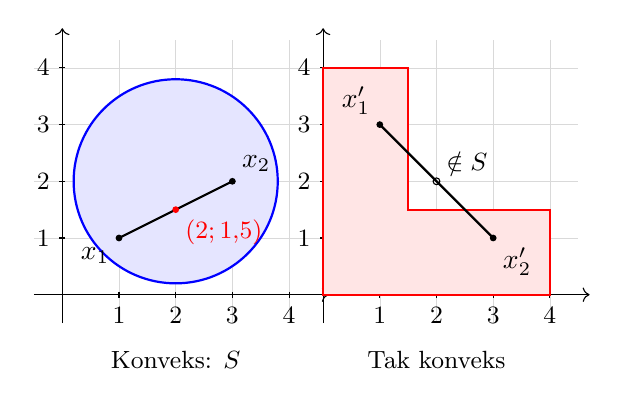
\begin{tikzpicture}[scale=0.72]
  \begin{scope}
    \draw[help lines, gray!30] (-0.5,-0.5) grid (4.5,4.5);
    \draw[->, thin] (-0.5,0) -- (4.7,0);
    \draw[->, thin] (0,-0.5) -- (0,4.7);
    \foreach \i in {1,2,3,4} {
      \draw (\i,0.05) -- (\i,-0.05) node[below] {\small \i};
      \draw (0.05,\i) -- (-0.05,\i) node[left] {\small \i};
    }
    \draw[thick, blue, fill=blue!10] (2,2) circle (1.8);
    \fill (1,1) circle (1.7pt) node[below left] {$x_1$};
    \fill (3,2) circle (1.7pt) node[above right] {$x_2$};
    \draw[thick] (1,1) -- (3,2);
    \fill[red] (2,1.5) circle (1.7pt)
      node[below right] {\small $(2;1{,}5)$};
    \node at (2,-1.15) {\small Konveks: $S$};
  \end{scope}

  \begin{scope}[xshift=4.6cm]
    \draw[help lines, gray!30] (-0.5,-0.5) grid (4.5,4.5);
    \draw[->, thin] (-0.5,0) -- (4.7,0);
    \draw[->, thin] (0,-0.5) -- (0,4.7);
    \foreach \i in {1,2,3,4} {
      \draw (\i,0.05) -- (\i,-0.05) node[below] {\small \i};
      \draw (0.05,\i) -- (-0.05,\i) node[left] {\small \i};
    }
    \draw[thick, red, fill=red!10]
      (0,0) -- (4,0) -- (4,1.5) -- (1.5,1.5)
      -- (1.5,4) -- (0,4) -- cycle;
    \fill (1,3) circle (1.7pt) node[above left] {$x_1'$};
    \fill (3,1) circle (1.7pt) node[below right] {$x_2'$};
    \draw[thick] (1,3) -- (3,1);
    \draw (2,2) circle (1.7pt);
    \node[above right] at (2,2) {\small $\notin S$};
    \node at (2,-1.15) {\small Tak konveks};
  \end{scope}
\end{tikzpicture}
\caption{Contoh himpunan konveks (kiri) dan tak konveks (kanan).
Pada himpunan tak konveks, ruas garis antara $x_1'$ dan $x_2'$
melewati titik $(2,2)$ yang berada di luar himpunan.}
\label{fig:konveks}
\end{figure}


\subsection{Kombinasi Konveks dan Convex Hull}
\label{subsec:kombinasikonveks}

Konsep himpunan konveks dapat diperluas untuk mencampurkan lebih dari
dua titik. Campuran ini disebut \textit{kombinasi konveks} apabila
setiap bobot tidak negatif dan jumlah seluruh bobotnya sama dengan
satu.

\begin{definisi}[\citealp{boyd}]
\label{def:kombinasikonveks}
Untuk titik-titik $x_1,\dots,x_k\in\mathbb{R}^n$ dan skalar
$\theta_1,\dots,\theta_k$ yang memenuhi
$\theta_i\geq 0$ dan $\sum_{i=1}^{k}\theta_i=1$, titik
\begin{equation}
    \sum_{i=1}^{k}\theta_i x_i
    \label{eq:kombinasikonveks}
\end{equation}
disebut \textit{kombinasi konveks} dari $x_1,\dots,x_k$.
\end{definisi}

Kumpulan seluruh kombinasi konveks dari titik-titik dalam suatu
himpunan membentuk \textit{convex hull}, yaitu himpunan konveks
terkecil yang memuat himpunan tersebut.

\begin{definisi}[\citealp{boyd}]
\label{def:convexhull}
\textit{Convex hull} dari himpunan $S\subseteq\mathbb{R}^n$,
ditulis $\operatorname{conv}(S)$, didefinisikan sebagai
\begin{equation}
    \operatorname{conv}(S)
    =
    \left\{
    \sum_{i=1}^{k}\theta_i x_i
    \;\middle|\;
    \begin{array}{l}
    k\in\mathbb{N},\ x_i\in S,\ \theta_i\geq 0,\\
    \displaystyle\sum_{i=1}^{k}\theta_i=1
    \end{array}
    \right\},
    \label{eq:convexhull}
\end{equation}
sehingga $\operatorname{conv}(S)$ merupakan himpunan
konveks terkecil yang memuat $S$.
\end{definisi}


\subsection{Simpleks Probabilitas}
\label{subsec:simpleksprobabilitas}

Salah satu contoh penting yang berkaitan dengan kombinasi konveks
adalah \textit{simpleks probabilitas}, yaitu himpunan seluruh vektor
probabilitas untuk $V$ kategori. Setiap komponennya tidak negatif
dan jumlah seluruh komponennya sama dengan satu.

\begin{definisi}[\citealp{boyd}]
\label{def:simpleks}
\textit{Simpleks probabilitas} berdimensi $V-1$ didefinisikan sebagai
\begin{equation}
    \Delta^{V-1}
    =
    \left\{
    p=(p_1,\dots,p_V)^\top\in\mathbb{R}^{V}
    \;\middle|\;
    p_i\geq 0,\ 
    \sum_{i=1}^{V}p_i=1
    \right\}.
    \label{eq:simpleks}
\end{equation}
\end{definisi}

Simpleks probabilitas merupakan \textit{convex hull} dari vektor
indikator $e_1,\dots,e_V$ (Definisi~\ref{def:onehot}), yaitu
\begin{equation}
    \Delta^{V-1}
    =
    \operatorname{conv}\{e_1,\dots,e_V\}.
\end{equation}
Setiap vektor probabilitas $p\in\Delta^{V-1}$ dapat dinyatakan
sebagai kombinasi konveks
\begin{equation}
    p=\sum_{i=1}^{V}p_i e_i.
\end{equation}
Dalam representasi ini, setiap vektor indikator merupakan titik
sudut simpleks yang menyatakan probabilitas satu pada satu kategori,
sedangkan titik-titik lainnya menyatakan distribusi probabilitas
yang tersebar di antara beberapa kategori.

Gambar~\ref{fig:simpleks} mengilustrasikan simpleks probabilitas
untuk $V=3$ kategori. Karena $p_1+p_2+p_3=1$, simpleks tersebut
dapat digambarkan pada bidang $(p_1,p_2)$ dengan
$p_3=1-p_1-p_2$.

\begin{figure}[H]
\centering
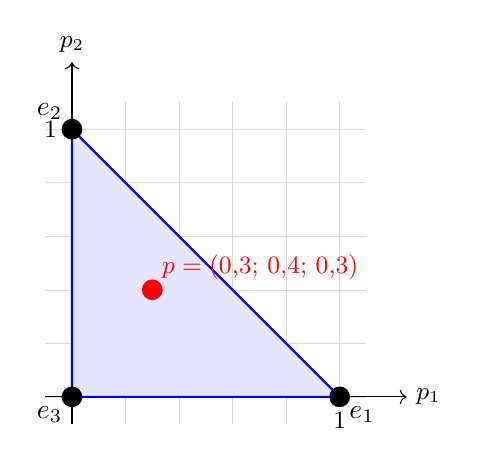
\begin{tikzpicture}[scale=3.4]
  \draw[help lines, gray!30, step=0.2] (-0.1,-0.1) grid (1.1,1.1);
  \draw[->, thin] (-0.1,0) -- (1.25,0) node[right] {\small $p_1$};
  \draw[->, thin] (0,-0.1) -- (0,1.25) node[above] {\small $p_2$};
  \draw (1,0.02) -- (1,-0.02) node[below] {\small $1$};
  \draw (0.02,1) -- (-0.02,1) node[left] {\small $1$};

  \draw[thick, blue, fill=blue!10] (1,0) -- (0,1) -- (0,0) -- cycle;
  \fill (1,0) circle (1.1pt) node[below right] {$e_1$};
  \fill (0,1) circle (1.1pt) node[above left] {$e_2$};
  \fill (0,0) circle (1.1pt) node[below left] {$e_3$};
  \fill[red] (0.3,0.4) circle (1.1pt)
    node[above right] {\small $p=(0{,}3;\,0{,}4;\,0{,}3)$};
\end{tikzpicture}
\caption{Simpleks probabilitas $\Delta^2$ untuk $V=3$ kategori
pada bidang $(p_1,p_2)$. Titik sudut $e_1,e_2,e_3$ menyatakan
distribusi yang pasti pada satu kategori, sedangkan titik di bagian
dalam menyatakan distribusi campuran.}
\label{fig:simpleks}
\end{figure}



\section{Entropi}
\label{sec:entropi}

\subsection{Entropi Shannon}
\label{subsec:entropishannon}

Entropi Shannon mengukur ketidakpastian suatu variabel random
diskret. Misalkan $X$ merupakan variabel random diskret dengan
ruang nilai $\mathcal{X}$ dan fungsi massa probabilitas $p(x)$.
Entropi Shannon didefinisikan sebagai berikut.

\begin{definisi}[\citealp{cover}]
\label{def:entropishannon}
Entropi Shannon dari variabel random diskret $X$ adalah
\begin{equation}
    H(X)=-\sum_{x\in\mathcal{X}}p(x)\log p(x),
    \label{eq:entropishannon}
\end{equation}
dengan konvensi $0\log 0:=0$.
\end{definisi}

\subsection{Batas Entropi}
\label{subsec:batasentropi}

Untuk variabel random diskret $X$ dengan ruang nilai berhingga
$\mathcal{X}$, entropi Shannon memenuhi batas berikut
\citep{cover}.

\begin{equation}
    0\leq H(X)\leq\log|\mathcal{X}|.
    \label{eq:batasentropi}
\end{equation}

Batas bawah dicapai jika dan hanya jika distribusi probabilitas
$X$ terkonsentrasi pada satu nilai, sedangkan batas atas dicapai
jika dan hanya jika distribusi probabilitas $X$ seragam pada
$\mathcal{X}$.


\section{Inferensi Bayes}
\label{sec:bayes}

Inferensi Bayes merupakan pendekatan untuk melakukan inferensi terhadap
parameter yang tidak diketahui dengan menggabungkan informasi awal
mengenai parameter dan informasi yang diperoleh dari data. Informasi
awal dinyatakan melalui distribusi prior, sedangkan informasi dari data
dinyatakan melalui likelihood. Penggabungan keduanya menghasilkan
distribusi posterior yang menggambarkan ketidakpastian parameter setelah
data diamati \citep{casella}.

\subsection{Definisi Bayes: Prior, Likelihood, dan Posterior}
\label{subsec:definisibayes}

\begin{definisi}[Rumus Bayes; \citealp{casella}]
\label{def:bayes}
Misalkan $\theta$ merupakan parameter dan $Y$ merupakan variabel random
yang menghasilkan data $y$. Jika $f(\theta)$ merupakan distribusi prior
dan $f(y\mid\theta)$ merupakan fungsi massa peluang atau fungsi kepadatan
bersyarat dari $Y$ diberikan $\theta$, maka distribusi posterior
$\theta$ setelah data $y$ diamati adalah
\begin{equation}
f(\theta\mid y)
=
\frac{f(y\mid\theta)f(\theta)}{f(y)}.
\label{eq:bayes}
\end{equation}
Untuk parameter kontinu, evidence $f(y)$ diperoleh melalui
\begin{equation}
f(y)
=
\int f(y\mid\theta)f(\theta)\,d\theta.
\label{eq:evidencekontinu}
\end{equation}
Untuk parameter diskret, integral digantikan dengan penjumlahan.
\end{definisi}

Pada Persamaan~\eqref{eq:bayes}, $f(\theta)$ merupakan prior,
$f(y\mid\theta)$ merupakan likelihood, $f(y)$ merupakan evidence,
dan $f(\theta\mid y)$ merupakan posterior. Evidence berfungsi sebagai
konstanta normalisasi agar posterior merupakan distribusi probabilitas
yang sah. Karena evidence tidak bergantung pada $\theta$, posterior
juga dapat dinyatakan secara proporsional sebagai
\begin{equation}
f(\theta\mid y)
\propto f(y\mid\theta)f(\theta).
\label{eq:bayesproporsional}
\end{equation}
Bentuk proporsional ini memudahkan penentuan posterior ketika hasil
perkalian likelihood dan prior sudah dapat dikenali sebagai kernel
suatu keluarga distribusi.


\subsection{Prior Konjugat}
\label{subsec:priorkonjugat}

\begin{definisi}[\citealp{casella}]
\label{def:priorkonjugat}
Keluarga distribusi prior $\mathcal{F}$ disebut konjugat terhadap
likelihood $f(y\mid\theta)$ apabila posterior yang diperoleh dari
setiap prior dalam $\mathcal{F}$ juga termasuk dalam keluarga
distribusi $\mathcal{F}$.
\end{definisi}

Kekonjugatan memungkinkan posterior dinyatakan dalam bentuk tertutup
tanpa harus menghitung evidence secara eksplisit. Salah satu contoh
yang relevan dalam penelitian ini adalah kekonjugatan Dirichlet--Multinomial.


\subsection{Kekonjugatan Dirichlet--Multinomial}
\label{subsec:konjugasidirichletmultinomial}

\begin{definisi}[\citealp{gelman}]
\label{def:konjugasidirichletmultinomial}
Misalkan vektor probabilitas
$\theta=(\theta_1,\ldots,\theta_V)^\top$ memiliki prior
\[
\theta\sim\operatorname{Dir}(\alpha),
\qquad
\alpha=(\alpha_1,\ldots,\alpha_V)^\top,
\]
dengan $\alpha_i>0$. Jika, diberikan $\theta$, vektor frekuensi
kategori $\bm{c}=(c_1,\ldots,c_V)^\top$ mengikuti distribusi
Multinomial dengan ukuran sampel $n$, maka posteriornya adalah
\begin{equation}
\theta\mid\bm{c}
\sim\operatorname{Dir}(\alpha+\bm{c}).
\label{eq:konjugasidirichletmultinomial}
\end{equation}
\end{definisi}

Hasil tersebut dapat diturunkan menggunakan Rumus Bayes dengan
mengalikan likelihood Multinomial dan prior Dirichlet. Berdasarkan
Persamaan~\eqref{eq:multinomial}, fungsi likelihood untuk vektor
frekuensi $\bm{c}$ adalah
\begin{equation}
f(\bm{c}\mid\theta)
=
\frac{n!}{\prod_{i=1}^{V}c_i!}
\prod_{i=1}^{V}\theta_i^{c_i},
\label{eq:likelihoodmultinomial}
\end{equation}
dengan $\sum_{i=1}^{V}c_i=n$. Sementara itu, berdasarkan
Persamaan~\eqref{eq:dirichlet}, fungsi kepadatan prior Dirichlet
adalah
\begin{equation}
f(\theta)
=
\frac{1}{B(\alpha)}
\prod_{i=1}^{V}\theta_i^{\alpha_i-1},
\label{eq:priorlengkap}
\end{equation}
dengan $B(\alpha)$ merupakan konstanta normalisasi distribusi
Dirichlet.

Menurut Rumus Bayes pada Persamaan~\eqref{eq:bayes}, posterior
sebanding dengan perkalian likelihood dan prior. Oleh karena itu,
diperoleh
\begin{align}
f(\theta\mid\bm{c})
&\propto f(\bm{c}\mid\theta)f(\theta)
\nonumber\\
&=
\frac{n!}{\prod_{i=1}^{V}c_i!}
\frac{1}{B(\alpha)}
\left(\prod_{i=1}^{V}\theta_i^{c_i}\right)
\left(\prod_{i=1}^{V}\theta_i^{\alpha_i-1}\right).
\label{eq:perkalianlikelihoodprior}
\end{align}

Pada Persamaan~\eqref{eq:perkalianlikelihoodprior}, faktor
$\frac{n!}{\prod_{i=1}^{V}c_i!}$ dan $\frac{1}{B(\alpha)}$
tidak bergantung pada $\theta$. Karena itu, kedua faktor tersebut
dapat diserap ke dalam konstanta proporsionalitas. Selanjutnya,
menggunakan sifat perkalian berpangkat
$x^a x^b=x^{a+b}$, diperoleh
\begin{align}
f(\theta\mid\bm{c})
&\propto
\prod_{i=1}^{V}
\theta_i^{c_i}\theta_i^{\alpha_i-1}
\nonumber\\
&=
\prod_{i=1}^{V}
\theta_i^{\alpha_i+c_i-1}.
\label{eq:kernelposterior}
\end{align}

Bentuk pada Persamaan~\eqref{eq:kernelposterior} sama dengan
bentuk kernel distribusi Dirichlet, yaitu hasil kali setiap
komponen probabilitas yang dipangkatkan dengan parameter
distribusinya dikurangi satu. Dengan membandingkannya dengan
fungsi kepadatan Dirichlet, parameter posterior dapat diidentifikasi
sebagai $\alpha_i+c_i$ untuk setiap kategori $i$.

Agar menjadi fungsi kepadatan probabilitas, kernel
tersebut harus dinormalisasi. Konstanta normalisasinya adalah
$B(\alpha+\bm{c})$, sehingga posterior lengkapnya menjadi
\begin{equation}
f(\theta\mid\bm{c})
=
\frac{1}{B(\alpha+\bm{c})}
\prod_{i=1}^{V}
\theta_i^{\alpha_i+c_i-1}
\label{eq:posteriorlengkap}
\end{equation}
dan diperoleh
$\theta\mid\bm{c}\sim\operatorname{Dir}(\alpha+\bm{c})$,
sebagaimana dinyatakan pada
Persamaan~\eqref{eq:konjugasidirichletmultinomial}. Hasil ini
menunjukkan bahwa keluarga prior Dirichlet tetap menjadi keluarga
posterior setelah pengamatan mengikuti likelihood Multinomial.


Secara intuitif, pembaruan posterior menambahkan frekuensi
pengamatan $c_i$ pada parameter prior $\alpha_i$. Untuk satu
pengamatan pada kategori $y$, vektor frekuensinya merupakan
vektor indikator $e_y$, yang didefinisikan sebagai
\[
(e_y)_i=
\begin{cases}
1, & i=y,\\
0, & i\neq y.
\end{cases}
\]
Oleh karena itu, pembaruan posterior untuk satu pengamatan adalah
\begin{equation}
\theta\mid y
\sim\operatorname{Dir}(\alpha+e_y).
\label{eq:posterioronehot}
\end{equation}
Artinya, parameter prior untuk kategori yang diamati bertambah
satu, sedangkan parameter kategori lainnya tidak berubah.

\begin{definisi}[\citealp{gelman}]
\label{def:pseudocount}
Parameter prior $\alpha_i$ disebut \textit{pseudo-count} kategori
$i$, sedangkan
\[
\alpha_0=\sum_{i=1}^{V}\alpha_i
\]
disebut massa konsentrasi prior. Pembaruan
$\alpha_i\mapsto\alpha_i+c_i$ menambahkan frekuensi pengamatan
kategori $i$ pada pseudo-count kategori tersebut.
\end{definisi}

Berdasarkan rumus ekspektasi distribusi Dirichlet pada
Persamaan~\eqref{eq:ekspektasidirichlet}, ekspektasi komponen
posterior diperoleh dengan mengganti parameter prior
$\alpha_i$ menjadi parameter posterior $\alpha_i+c_i$:
\begin{align}
\mathbb{E}[\theta_i\mid\bm{c}]
&=
\frac{\alpha_i+c_i}
{\sum_{j=1}^{V}(\alpha_j+c_j)}
\nonumber\\
&=
\frac{\alpha_i+c_i}{\alpha_0+n},
\qquad i=1,\ldots,V,
\label{eq:ekspektasiposterior}
\end{align}
karena $\sum_{i=1}^{V}c_i=n$. Persamaan ini menunjukkan bahwa
rerata posterior ditentukan oleh pseudo-count awal dan frekuensi
pengamatan, sedangkan penyebutnya merupakan total konsentrasi
setelah pembaruan.

\subsection{Rerata Posterior sebagai Estimator Bayes}
\label{subsec:estimatorbayes}

\begin{definisi}[\citealp{casella}]
\label{def:risikokuadratik}
Misalkan $\theta\in\mathbb{R}^{V}$ merupakan parameter random
dan $\delta=\delta(y)\in\mathbb{R}^{V}$ merupakan penduga
parameter berdasarkan data $y$. Risiko posterior dengan \textit{squared loss} didefinisikan sebagai
\begin{equation}
R(\delta\mid y)
=
\mathbb{E}\left[
\lVert\theta-\delta\rVert_2^2
\mid y
\right].
\label{eq:risikokuadratik}
\end{equation}
Penduga yang meminimumkan risiko posterior tersebut disebut
estimator Bayes di bawah \textit{squared loss}.
\end{definisi}

Untuk menunjukkan bahwa rerata posterior merupakan estimator
Bayes di bawah \textit{squared loss}, definisikan
$\mu_i=\mathbb{E}[\theta_i\mid y]$. Karena kuadrat norma
Euclidean merupakan jumlah kuadrat setiap komponen, risiko
posterior dapat dituliskan sebagai
\begin{align}
R(\delta\mid y)
&=
\mathbb{E}\left[
\sum_{i=1}^{V}(\theta_i-\delta_i)^2
\mid y
\right]
\nonumber\\
&=
\sum_{i=1}^{V}
\mathbb{E}\left[
(\theta_i-\delta_i)^2\mid y
\right].
\label{eq:risikokomponen}
\end{align}
Langkah kedua menggunakan linearitas ekspektasi, yaitu
ekspektasi dari jumlah berhingga sama dengan jumlah ekspektasi
masing-masing suku.

Selanjutnya, setiap selisih $\theta_i-\delta_i$ dapat diuraikan
dengan menambahkan dan mengurangkan rerata posterior $\mu_i$:
\begin{equation}
\theta_i-\delta_i
=
(\theta_i-\mu_i)+(\mu_i-\delta_i).
\label{eq:uraianselisih}
\end{equation}
Dengan menguadratkan kedua ruas, diperoleh
\begin{align}
(\theta_i-\delta_i)^2
&=
(\theta_i-\mu_i)^2
+2(\theta_i-\mu_i)(\mu_i-\delta_i)
\nonumber\\
&\quad
+(\mu_i-\delta_i)^2.
\label{eq:kuadratselisih}
\end{align}
Mengambil ekspektasi bersyarat pada data $y$ menghasilkan
\begin{align}
&\mathbb{E}\left[
(\theta_i-\delta_i)^2\mid y
\right]
\nonumber\\
&=
\mathbb{E}\left[
(\theta_i-\mu_i)^2\mid y
\right]
\nonumber\\
&\quad+
2(\mu_i-\delta_i)
\mathbb{E}\left[
\theta_i-\mu_i\mid y
\right]
+(\mu_i-\delta_i)^2.
\label{eq:ekspektasikuadrat}
\end{align}
Pada langkah ini, $\mu_i$ dan $\delta_i$ diperlakukan sebagai
konstanta karena keduanya ditentukan oleh distribusi posterior
setelah data $y$ diamati.

Berdasarkan definisi rerata posterior,
\begin{align}
\mathbb{E}\left[
\theta_i-\mu_i\mid y
\right]
&=
\mathbb{E}[\theta_i\mid y]-\mu_i
\nonumber\\
&=\mu_i-\mu_i=0.
\label{eq:rerataterpusat}
\end{align}
Akibatnya, suku silang pada
Persamaan~\eqref{eq:ekspektasikuadrat} bernilai nol.
Sementara itu, suku pertama merupakan varians posterior karena
$\mu_i=\mathbb{E}[\theta_i\mid y]$. Dengan demikian,
\begin{equation}
\mathbb{E}\left[
(\theta_i-\delta_i)^2\mid y
\right]
=
\operatorname{Var}(\theta_i\mid y)
+(\delta_i-\mu_i)^2.
\label{eq:dekomposisirisiko}
\end{equation}

Substitusi Persamaan~\eqref{eq:dekomposisirisiko} ke dalam
Persamaan~\eqref{eq:risikokomponen} memberikan
\begin{align}
R(\delta\mid y)
&=
\sum_{i=1}^{V}
\operatorname{Var}(\theta_i\mid y)
+
\sum_{i=1}^{V}(\delta_i-\mu_i)^2.
\label{eq:risikoterurai}
\end{align}
Suku pertama tidak bergantung pada penduga $\delta$, sedangkan
suku kedua merupakan jumlah kuadrat yang selalu tidak negatif.
Suku kedua mencapai nilai minimum nol apabila
$\delta_i=\mu_i$ untuk setiap $i$. Oleh karena itu, risiko
posterior minimum dicapai oleh
\begin{equation}
\delta^*
=
\mathbb{E}[\theta\mid y]
=
\begin{pmatrix}
\mathbb{E}[\theta_1\mid y]\\
\vdots\\
\mathbb{E}[\theta_V\mid y]
\end{pmatrix}.
\label{eq:estimatorbayes}
\end{equation}
Rerata posterior merupakan estimator Bayes
di bawah \textit{squared loss}.

Dalam konteks prior Dirichlet dan likelihood Multinomial,
Persamaan~\eqref{eq:ekspektasiposterior} memberikan bentuk
eksplisit estimator Bayes tersebut:
\begin{equation}
\delta_i^*
=
\frac{\alpha_i+c_i}{\alpha_0+n},
\qquad i=1,\ldots,V.
\label{eq:estimatorbayesdirichlet}
\end{equation}
Hasil ini menjadi landasan matematis untuk menggunakan rerata
posterior sebagai bobot campuran dalam metode Mixture of Inputs.



\section{Model Bahasa dan Arsitektur \textit{Transformer}}
\label{sec:transformer}

\subsection{Model Bahasa Autoregresif}
\label{subsec:autoregresif}

\begin{definisi}[\citealp{goodfellow}]
\label{def:modelbahasa}
Misalkan $\mathcal{V}=\{1,\dots,V\}$ kosakata (\textit{vocabulary})
berukuran $V$, dan $x=(x_1,\dots,x_n)$ barisan token dengan $x_t\in
\mathcal{V}$. \textit{Model bahasa} (\textit{language model}) adalah
distribusi peluang atas barisan token, difaktorkan menurut aturan rantai
peluang sebagai
\begin{equation}
  p(x) = \prod_{t=1}^{n} p(x_t \mid x_{<t}),
  \label{eq:autoregresif}
\end{equation}
dengan $x_{<t}=(x_1,\dots,x_{t-1})$. Model yang memfaktorkan peluangnya
demikian --- token ke-$t$ dibangkitkan bergantung pada seluruh token
sebelumnya --- disebut \textit{autoregresif}.
\end{definisi}

Persamaan~\eqref{eq:autoregresif} adalah penerapan berulang aturan rantai
peluang. Untuk $n=3$ misalnya, produknya terurai menjadi tiga faktor,
\begin{equation}
  p(x_1,x_2,x_3) = p(x_1)\,p(x_2\mid x_1)\,p(x_3\mid x_1,x_2),
  \label{eq:autoregresifcontoh}
\end{equation}
dengan $p(x_1)=p(x_1\mid x_{<1})$ memakai $x_{<1}=\varnothing$ (barisan
kosong, tidak ada token sebelum token pertama). Setiap faktor pada
Persamaan~\eqref{eq:autoregresifcontoh} adalah distribusi atas $V$
kategori yang bersyarat pada token-token sebelumnya, sehingga membangkitkan
barisan $x$ berarti membangkitkan token satu per satu secara berurutan:
$x_1$ terlebih dahulu, kemudian $x_2$ dengan $x_1$ diketahui, dan
seterusnya.


\subsection{Jaringan Saraf, Fungsi Aktivasi, dan Fungsi \textit{Softmax}}
\label{subsec:softmax}

Komponen dasar jaringan saraf tiruan adalah lapisan (\textit{layer})
yang memetakan masukan $u\in\mathbb{R}^{m}$ menjadi keluaran
$\sigma(Wu+b)$, dengan $W$ dan $b$ merupakan parameter yang
dipelajari, sedangkan $\sigma$ adalah fungsi aktivasi taklinear,
seperti ReLU atau \textit{tanh}. Fungsi aktivasi memungkinkan
tumpukan lapisan memodelkan hubungan yang lebih kompleks daripada
kombinasi linear semata \citep{goodfellow}. Arsitektur
\textit{Transformer} juga tersusun atas rangkaian lapisan yang
melibatkan operasi linear dan fungsi aktivasi.

Pada model bahasa, lapisan keluaran menghasilkan vektor
\textit{logit} $\ell=(\ell_1,\ldots,\ell_V)^\top\in\mathbb{R}^V$,
dengan setiap $\ell_i$ merupakan skor untuk token ke-$i$ dari
kosakata berukuran $V$. Agar skor tersebut dapat digunakan sebagai
distribusi probabilitas, diperlukan fungsi \textit{softmax}.

\begin{definisi}[\citealp{goodfellow}]
\label{def:softmax}
Fungsi \textit{softmax} memetakan vektor logit
$\ell\in\mathbb{R}^V$ menjadi vektor probabilitas
$p=\operatorname{softmax}(\ell)\in\Delta^{V-1}$, dengan komponen
\begin{equation}
p_i=\frac{\exp(\ell_i)}
{\sum_{j=1}^{V}\exp(\ell_j)},
\qquad i=1,\ldots,V.
\label{eq:softmax}
\end{equation}
Setiap komponen $p_i$ menyatakan probabilitas kategori ke-$i$.
Nilainya positif dan jumlah seluruh komponennya sama dengan satu,
sehingga $p$ merupakan distribusi probabilitas pada simpleks
$\Delta^{V-1}$ (Definisi~\ref{def:simpleks}).
\end{definisi}

Dalam penerapannya, fungsi \textit{softmax} dapat menggunakan
parameter suhu (\textit{temperature}) $T>0$ dengan mengganti logit
$\ell_i$ menjadi $\ell_i/T$:
\begin{equation}
p_i=\frac{\exp(\ell_i/T)}
{\sum_{j=1}^{V}\exp(\ell_j/T)}.
\label{eq:softmax-temperature}
\end{equation}
Parameter $T$ mengatur tingkat ketajaman distribusi. Ketika
$T$ mengecil, perbedaan antarlogit menjadi lebih berpengaruh
sehingga probabilitas cenderung terkonsentrasi pada kategori
dengan logit terbesar. Sebaliknya, ketika $T$ membesar, perbedaan
tersebut semakin berkurang dan distribusi mendekati seragam.

Gambar~\ref{fig:softmax} mengilustrasikan pengaruh suhu terhadap
bentuk distribusi.

\begin{figure}[H]
\centering
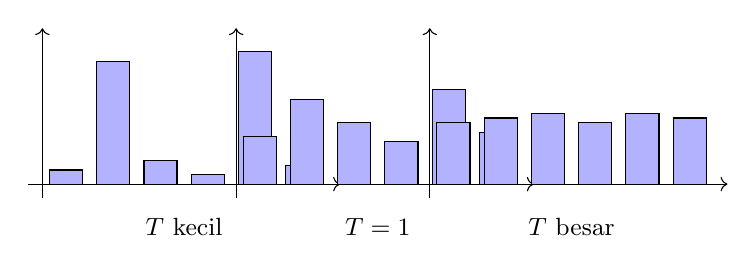
\begin{tikzpicture}[scale=0.6]
  \begin{scope}
    \draw[->, thin] (-0.3,0) -- (6.3,0);
    \draw[->, thin] (0,-0.3) -- (0,3.3);
    \foreach \x/\h in {0.5/0.3, 1.5/2.6, 2.5/0.5, 3.5/0.2, 4.5/2.8, 5.5/0.4} {
      \draw[fill=blue!30] (\x-0.35,0) rectangle (\x+0.35,\h);
    }
    \node at (3,-0.9) {\small $T$ kecil};
  \end{scope}

  \begin{scope}[xshift=4.1cm]
    \draw[->, thin] (-0.3,0) -- (6.3,0);
    \draw[->, thin] (0,-0.3) -- (0,3.3);
    \foreach \x/\h in {0.5/1.0, 1.5/1.8, 2.5/1.3, 3.5/0.9, 4.5/2.0, 5.5/1.1} {
      \draw[fill=blue!30] (\x-0.35,0) rectangle (\x+0.35,\h);
    }
    \node at (3,-0.9) {\small $T=1$};
  \end{scope}

  \begin{scope}[xshift=8.2cm]
    \draw[->, thin] (-0.3,0) -- (6.3,0);
    \draw[->, thin] (0,-0.3) -- (0,3.3);
    \foreach \x/\h in {0.5/1.3, 1.5/1.4, 2.5/1.5, 3.5/1.3, 4.5/1.5, 5.5/1.4} {
      \draw[fill=blue!30] (\x-0.35,0) rectangle (\x+0.35,\h);
    }
    \node at (3,-0.9) {\small $T$ besar};
  \end{scope}
\end{tikzpicture}
\caption{Ilustrasi pengaruh suhu $T$ terhadap distribusi
$p=\operatorname{softmax}(\ell/T)$ untuk logit yang sama.
Suhu kecil menghasilkan distribusi yang lebih tajam, sedangkan
suhu besar menghasilkan distribusi yang lebih mendekati seragam.}
\label{fig:softmax}
\end{figure}




\subsection{Mekanisme Atensi dan \textit{KV-Cache}}
\label{subsec:atensi}

\textit{Transformer} memproses representasi token melalui mekanisme
atensi (\textit{attention}), yang memungkinkan representasi setiap
posisi dibentuk dari kombinasi berbobot representasi posisi-posisi
lain yang relevan.

\begin{definisi}[\citealp{vaswani}]
\label{def:atensi}
Untuk matriks \textit{query} (\textit{query}) $Q\in\mathbb{R}^{n\times d_k}$,
\textit{key} (\textit{key}) $K\in\mathbb{R}^{n\times d_k}$, dan nilai
(\textit{value}) $V\in\mathbb{R}^{n\times d_v}$, mekanisme
\textit{atensi produk-titik berskala} (\textit{scaled dot-product
attention}) didefinisikan sebagai
\begin{equation}
\operatorname{Atensi}(Q,K,V)
=
\operatorname{softmax}
\left(\frac{QK^\top}{\sqrt{d_k}}\right)V,
\label{eq:atensi}
\end{equation}
dengan fungsi \textit{softmax} diterapkan pada setiap baris matriks.
\end{definisi}


\paragraph{Perkalian matriks (\textit{MatMul}).}
Operasi pertama menghitung $QK^\top$. Karena
$Q\in\mathbb{R}^{n\times d_k}$ dan
$K^\top\in\mathbb{R}^{d_k\times n}$, hasilnya merupakan matriks
berukuran $n\times n$. Setiap elemennya merupakan hasil kali titik
(\textit{dot product}) antara satu baris $Q$ dan satu baris $K$:
\begin{equation}
(QK^\top)_{ij}
=
\sum_{r=1}^{d_k}Q_{ir}K_{jr}.
\label{eq:atensi-matmul}
\end{equation}
Nilai tersebut mengukur kesesuaian antara \textit{query} pada posisi $i$
dan \textit{key} pada posisi $j$. Dengan demikian, matriks $QK^\top$
memuat skor kesesuaian setiap posisi terhadap seluruh posisi
lainnya.

\paragraph{Penskalaan (\textit{Scale}).}
Skor kesesuaian kemudian dibagi dengan $\sqrt{d_k}$:
\begin{equation}
S=\frac{QK^\top}{\sqrt{d_k}}.
\label{eq:atensi-scale}
\end{equation}
Pembagian ini mengendalikan besarnya skor sebelum fungsi
\textit{softmax} diterapkan. Ketika dimensi $d_k$ membesar,
hasil kali titik cenderung memiliki varians yang lebih besar
dengan asumsi komponen \textit{query} dan \textit{key} memiliki varians yang
terkendali dan tidak berkorelasi. Skor yang terlalu besar dapat
membuat distribusi \textit{softmax} terlalu terkonsentrasi.
Karena itu, faktor $\sqrt{d_k}$ membantu menjaga skala skor
agar proses pembobotan lebih stabil.

\paragraph{Fungsi \textit{softmax}.}
Fungsi \textit{softmax} diterapkan pada setiap baris matriks $S$
untuk mengubah skor kesesuaian menjadi bobot probabilitas:
\begin{equation}
A_{ij}
=
\frac{\exp(S_{ij})}
{\sum_{r=1}^{n}\exp(S_{ir})}.
\label{eq:atensi-softmax}
\end{equation}
Setiap elemen $A_{ij}$ menunjukkan bobot posisi $j$ ketika
representasi posisi $i$ dibentuk. Untuk setiap baris $i$,
berlaku $A_{ij}\geq 0$ dan $\sum_{j=1}^{n}A_{ij}=1$.
Dengan demikian, bobot tersebut dapat digunakan untuk
menggabungkan informasi dari berbagai posisi.

\paragraph{Pembobotan nilai (\textit{MatMul}).}
Operasi terakhir mengalikan matriks bobot $A$ dengan matriks
\textit{value} $V$:
\begin{equation}
O=AV.
\label{eq:atensi-output}
\end{equation}
Karena $A\in\mathbb{R}^{n\times n}$ dan
$V\in\mathbb{R}^{n\times d_v}$, keluaran
$O\in\mathbb{R}^{n\times d_v}$. Setiap baris keluaran merupakan
kombinasi berbobot baris-baris $V$, dengan bobot yang ditentukan
oleh skor kesesuaian pada tahap sebelumnya. Oleh karena itu,
representasi keluaran menggabungkan informasi dari posisi-posisi
yang memperoleh bobot atensi lebih besar.

Dalam praktiknya, operasi atensi dapat dilakukan pada beberapa
\textit{head} dengan proyeksi dan dimensi masing-masing, kemudian
hasilnya digabungkan melalui mekanisme
\textit{multi-head attention}.

Gambar~\ref{fig:atensi} mengilustrasikan urutan operasi tersebut.

\begin{figure}[H]
\centering
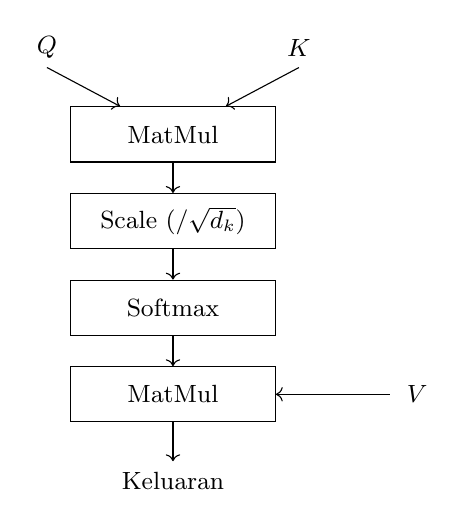
\begin{tikzpicture}[scale=1, every node/.style={font=\small}]
  \node[draw, minimum width=2.6cm, minimum height=0.7cm] (mm1) at (0,0) {MatMul};
  \node[draw, minimum width=2.6cm, minimum height=0.7cm] (sc) at (0,-1.1) {Scale ($/\sqrt{d_k}$)};
  \node[draw, minimum width=2.6cm, minimum height=0.7cm] (sm) at (0,-2.2) {Softmax};
  \node[draw, minimum width=2.6cm, minimum height=0.7cm] (mm2) at (0,-3.3) {MatMul};
  \draw[->] (mm1) -- (sc);
  \draw[->] (sc) -- (sm);
  \draw[->] (sm) -- (mm2);
  \draw[->] (0,-3.65) -- (0,-4.15);
  \node at (0,-4.4) {Keluaran};
  \node at (-1.6,1.1) {$Q$};
  \node at (1.6,1.1) {$K$};
  \draw[->] (-1.6,0.85) -- (mm1);
  \draw[->] (1.6,0.85) -- (mm1);
  \node at (3.1,-3.3) {$V$};
  \draw[->] (2.75,-3.3) -- (mm2);
\end{tikzpicture}
\caption{Alur perhitungan atensi produk-titik berskala pada
Persamaan~\eqref{eq:atensi}, mengikuti diagram \citet{vaswani}.}
\label{fig:atensi}
\end{figure}

Pada pembangkitan teks autoregresif, token dihasilkan satu per
satu. Untuk setiap lapisan, representasi token yang telah diproses
menghasilkan matriks \textit{key} dan \textit{value} yang dapat digunakan kembali
pada langkah berikutnya. Tanpa penyimpanan, model perlu menghitung
ulang \textit{key} dan \textit{value} token-token sebelumnya pada setiap langkah.

\begin{definisi}
\label{def:kvcache}
\textit{KV-cache} pada langkah ke-$t$ menyimpan matriks \textit{key} dan
\textit{value} untuk token-token sebelumnya pada setiap lapisan $l$:
\begin{equation}
\mathcal{M}_t^{(l)}
=
\left\{K_{1:t-1}^{(l)},V_{1:t-1}^{(l)}\right\}.
\label{eq:kvcache}
\end{equation}
Pada langkah $t$, \textit{key} dan \textit{value} token baru dihitung lalu
digabungkan dengan cache yang telah tersimpan. Dengan demikian,
model tidak perlu menghitung ulang \textit{key} dan \textit{value} seluruh
token sebelumnya.
\end{definisi}



\section{Strategi Pengambilan Sampel Token}
\label{sec:sampling}

Setelah distribusi probabilitas token
$p=\operatorname{softmax}(\ell/T)\in\Delta^{V-1}$
diperoleh (Persamaan~\eqref{eq:softmax}), model perlu menentukan
token berikutnya $x_t$ berdasarkan distribusi tersebut. Salah satu
cara adalah \textit{greedy decoding}, yaitu memilih token dengan
probabilitas terbesar,
\begin{equation}
x_t=\operatorname*{arg\,max}_{i\in\mathcal{V}}p_i.
\label{eq:greedy}
\end{equation}
Strategi ini bersifat deterministik untuk distribusi yang sama.
Alternatifnya, model dapat mengambil sampel dari distribusi
kategorik,
\begin{equation}
x_t\sim\operatorname{Kategorik}(p),
\label{eq:categorical-sampling}
\end{equation}
sehingga peluang terpilihnya setiap token sebanding dengan
probabilitasnya. Berbeda dari \textit{greedy decoding}, strategi ini
memungkinkan token dengan probabilitas lebih rendah tetap terpilih.
Namun, sampling langsung dari $p$ juga memungkinkan token dengan
probabilitas sangat kecil terpilih.

Untuk membatasi pilihan token, distribusi probabilitas dapat
dipotong sebelum sampling dilakukan. Dua strategi yang umum
digunakan adalah \textit{top-k sampling} dan \textit{nucleus
sampling} (\textit{top-p sampling}).

\begin{definisi}[\citealp{holtzman}]
\label{def:topk}
Untuk $k\in\{1,\ldots,V\}$, misalkan
$\mathcal{I}_k\subseteq\mathcal{V}$ merupakan himpunan $k$ token
dengan probabilitas terbesar. Pada \textit{top-k sampling},
probabilitas token di luar himpunan tersebut dibuat nol, sedangkan
probabilitas token yang tersisa dinormalisasi ulang:
\begin{equation}
\widetilde p_i=
\begin{cases}
\dfrac{p_i}{\sum_{j\in\mathcal{I}_k}p_j},
& i\in\mathcal{I}_k,\\[1.5ex]
0, & i\notin\mathcal{I}_k.
\end{cases}
\label{eq:topk}
\end{equation}
Dengan demikian, hanya $k$ token dengan probabilitas terbesar
yang dapat dipilih.

Pada \textit{nucleus sampling} atau \textit{top-p sampling},
himpunan token yang dipertahankan ditentukan berdasarkan
probabilitas kumulatif. Misalkan token diurutkan berdasarkan
probabilitas yang menurun. Himpunan $\mathcal{I}_p$ merupakan
himpunan terkecil yang memenuhi
\begin{equation}
\sum_{i\in\mathcal{I}_p}p_i\geq p,
\qquad p\in(0,1).
\label{eq:nucleus}
\end{equation}
Sama seperti pada \textit{top-k sampling}, probabilitas token
di luar $\mathcal{I}_p$ dibuat nol dan probabilitas token yang
tersisa dinormalisasi ulang sebelum sampling dilakukan.
Perbedaannya, \textit{top-k sampling} membatasi banyaknya token,
sedangkan \textit{top-p sampling} membatasi massa probabilitas
kumulatif yang dipertahankan.
\end{definisi}

\begin{figure}[H]
\centering
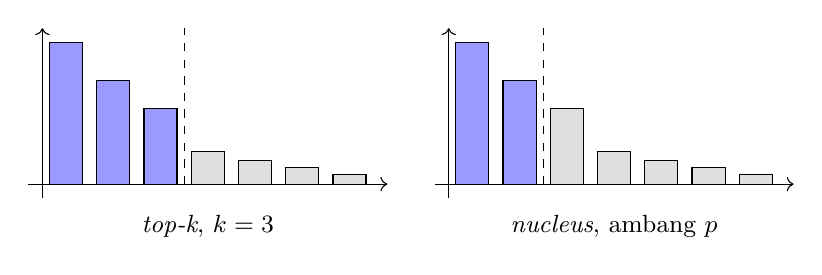
\begin{tikzpicture}[scale=0.6]
  \begin{scope}
    \draw[->, thin] (-0.3,0) -- (7.3,0);
    \draw[->, thin] (0,-0.3) -- (0,3.3);
    \draw[fill=blue!40]  (0.15,0) rectangle (0.85,3.0);
    \draw[fill=blue!40]  (1.15,0) rectangle (1.85,2.2);
    \draw[fill=blue!40]  (2.15,0) rectangle (2.85,1.6);
    \draw[fill=gray!25]  (3.15,0) rectangle (3.85,0.7);
    \draw[fill=gray!25]  (4.15,0) rectangle (4.85,0.5);
    \draw[fill=gray!25]  (5.15,0) rectangle (5.85,0.35);
    \draw[fill=gray!25]  (6.15,0) rectangle (6.85,0.2);
    \draw[dashed] (3.0,0) -- (3.0,3.3);
    \node at (3.5,-0.9) {\small \textit{top-k}, $k=3$};
  \end{scope}

  \begin{scope}[xshift=8.6cm]
    \draw[->, thin] (-0.3,0) -- (7.3,0);
    \draw[->, thin] (0,-0.3) -- (0,3.3);
    \draw[fill=blue!40]  (0.15,0) rectangle (0.85,3.0);
    \draw[fill=blue!40]  (1.15,0) rectangle (1.85,2.2);
    \draw[fill=gray!25]  (2.15,0) rectangle (2.85,1.6);
    \draw[fill=gray!25]  (3.15,0) rectangle (3.85,0.7);
    \draw[fill=gray!25]  (4.15,0) rectangle (4.85,0.5);
    \draw[fill=gray!25]  (5.15,0) rectangle (5.85,0.35);
    \draw[fill=gray!25]  (6.15,0) rectangle (6.85,0.2);
    \draw[dashed] (2.0,0) -- (2.0,3.3);
    \node at (3.5,-0.9) {\small \textit{nucleus}, ambang $p$};
  \end{scope}
\end{tikzpicture}
\caption{Perbandingan \textit{top-k sampling} (kiri, memotong pada
banyaknya kategori) dan \textit{nucleus sampling} (kanan, memotong pada
peluang kumulatif). Batang biru menandai kategori yang tersisa untuk
disampling ulang; batang abu-abu tersisih.}
\label{fig:sampling}
\end{figure}

Gambar~\ref{fig:sampling} mengilustrasikan perbedaan kedua strategi
tersebut. Pada \textit{top-k sampling}, jumlah token yang
dipertahankan ditentukan oleh $k$, sedangkan pada
\textit{top-p sampling}, jumlahnya dapat berubah mengikuti
bentuk distribusi probabilitas.

Dalam penelitian ini, strategi pengambilan token perlu dibedakan
berdasarkan penggunaannya. Pada medium komunikasi teks
(\texttt{text}), setiap agen menghasilkan keluaran teks melalui
proses generasi autoregresif. Implementasi menggunakan sampling
stokastik dengan parameter suhu $T=0{,}6$, \textit{top-k} sebesar
20, dan \textit{top-p} sebesar 0{,}95 sebagai nilai bawaan mesin
generasi. Pada setiap langkah, token berikutnya dipilih berdasarkan
distribusi yang telah dipengaruhi oleh suhu dan pembatasan
sampling tersebut. Proses ini diulang hingga generasi berakhir.
Keluaran teks dari agen perantara kemudian diberikan kepada agen
berikutnya sebagai konteks tekstual. Agen \textit{judger} juga
menggunakan mekanisme generasi teks ini untuk menghasilkan
jawaban akhir.



\section{Sistem Multi-Agen}
\label{sec:multiagen}

\subsection{Definisi Agen dan Sistem Multi-Agen}
\label{subsec:agen}

\begin{definisi}[\citealp{wooldridge2009}]
\label{def:agen}
\textit{Agen} (\textit{agent}) adalah entitas komputasi yang mengamati
lingkungannya melalui sensor dan bertindak terhadap lingkungan itu melalui
aktuator secara otonom --- tanpa campur tangan langsung manusia atau agen
lain pada setiap langkahnya --- untuk mencapai tujuan tertentu.
\end{definisi}

\begin{definisi}[\citealp{wooldridge2009}]
\label{def:mas}
\textit{Sistem multi-agen} (\textit{multi-agent system}, MAS) adalah
sistem yang tersusun atas dua atau lebih agen yang berinteraksi --- saling
bertukar informasi dan saling memengaruhi tindakan satu sama lain --- di
dalam lingkungan bersama.
\end{definisi}

Gambar~\ref{fig:agen} menggambarkan siklus persepsi--tindakan satu agen
terhadap lingkungannya.

\begin{figure}[H]
\centering
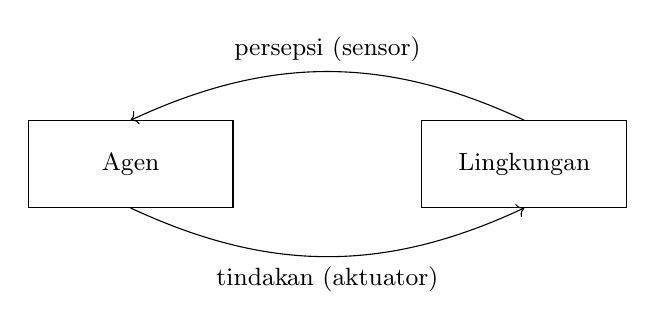
\begin{tikzpicture}[scale=1, every node/.style={font=\small}]
  \node[draw, minimum width=2.6cm, minimum height=1.1cm] (agen) at (0,0) {Agen};
  \node[draw, minimum width=2.6cm, minimum height=1.1cm] (ling) at (5,0) {Lingkungan};
  \draw[->] (ling.north) to[bend right=25] node[above]{persepsi (sensor)} (agen.north);
  \draw[->] (agen.south) to[bend right=25] node[below]{tindakan (aktuator)} (ling.south);
\end{tikzpicture}
\caption{Siklus persepsi--tindakan agen dan lingkungannya
\citep{wooldridge2009}. Pada sistem multi-agen, beberapa agen semacam ini
berbagi satu lingkungan dan dapat saling memengaruhi.}
\label{fig:agen}
\end{figure}

\subsection{Topologi Sekuensial dan Hierarkis}
\label{subsec:topologi}

Interaksi antaragen pada sistem multi-agen dapat diatur menurut berbagai
topologi koordinasi; dua yang paling mendasar adalah sekuensial dan
hierarkis \citep{wooldridge2009}. Pada topologi \textit{sekuensial}, agen
disusun sebagai rantai: keluaran satu agen menjadi masukan agen berikutnya,
sehingga informasi mengalir searah dari agen pertama hingga agen terakhir.
Pada topologi \textit{hierarkis}, satu agen berperan sebagai koordinator
yang mendelegasikan sub-tugas kepada beberapa agen bawahan dan
menggabungkan keluaran mereka. Gambar~\ref{fig:topologi} menggambarkan
kedua topologi tersebut.

\begin{figure}[H]
\centering
\begin{tikzpicture}[scale=1, every node/.style={draw, minimum width=1.3cm, minimum height=0.8cm, font=\small}]
  \node (a1) at (0,0) {$A_1$};
  \node (a2) at (1.8,0) {$A_2$};
  \node (a3) at (3.6,0) {$A_3$};
  \node (a4) at (5.4,0) {$A_4$};
  \draw[->] (a1) -- (a2);
  \draw[->] (a2) -- (a3);
  \draw[->] (a3) -- (a4);
  \node[draw=none] at (2.7,-1.0) {\small Sekuensial};

  \node (b0) at (9.6,0.9) {$A_0$};
  \node (b1) at (8.2,-0.6) {$A_1$};
  \node (b2) at (9.6,-0.6) {$A_2$};
  \node (b3) at (11.0,-0.6) {$A_3$};
  \draw[->] (b0) -- (b1);
  \draw[->] (b0) -- (b2);
  \draw[->] (b0) -- (b3);
  \draw[->] (b1) -- (b0);
  \draw[->] (b2) -- (b0);
  \draw[->] (b3) -- (b0);
  \node[draw=none] at (9.6,-1.6) {\small Hierarkis};
\end{tikzpicture}
\caption{Topologi sekuensial (kiri), rantai agen $A_1\to A_2\to A_3\to
A_4$, dan topologi hierarkis (kanan), koordinator $A_0$ yang
mendelegasikan ke $A_1,A_2,A_3$ dan menggabungkan keluarannya.}
\label{fig:topologi}
\end{figure}

\chapter{METODOLOGI PENELITIAN}

Penelitian ini membandingkan \textit{Mixture of Inputs} (MoI), yaitu
metode \textit{reasoning} melalui representasi laten, dengan tiga metode
lain: \code{raw} (\textit{input-output alignment}), \code{soft}
(\textit{Soft Thinking}), dan \code{sample} (\textit{discrete token}). Keempatnya
diterapkan pada sistem multi-agen yang berkomunikasi melalui transfer
\textit{KV-cache}, yang selanjutnya juga dibandingkan dengan sistem
multi-agen standar berbasis teks.

%==========================================================================
\section{Arsitektur Qwen3-8B}

\label{sec:m-arsitektur}

Qwen3-8B merupakan model bahasa autoregresif dengan arsitektur
\textit{Transformer decoder-only} \citep{qwen3} dengan
\textit{hidden layer} $L=36$ lapisan dan dimensi \textit{hidden state} $d=4096$.

Gambar~\ref{fig:m-latent-overview} memperlihatkan alur komputasi yang
digunakan sebagai dasar pembahasan. Teks \textit{input} diubah menjadi token(\textit{tokenization}), 
kemudian dipetakan melalui \textit{embedding} masukan $W_{\mathrm{in}}$ menjadi vektor.
Hasil \textit{embedding} tersebut diproses melalui seluruh blok \textit{decoder} 
hingga menghasilkan \textit{hidden state} $h_k$. \textit{Hidden state} dipetakan melalui \textit{output projection} $W_{\mathrm{out}}$ 
menjadi \textit{logit}, yang kemudian diubah menjadi \textit{probability} melalui fungsi \textit{softmax}.
Probabilitas digunakan untuk menghitung bobot $w_k$ yang digunakan untuk membentuk representasi laten $\tilde{z}_k$.
Representasi laten tersebut kemudian dinormalisasi menjadi $z_k$ sebelum dikembalikan ke \textit{embedding} masukan untuk langkah berikutnya.

\begin{figure}[H]
\centering
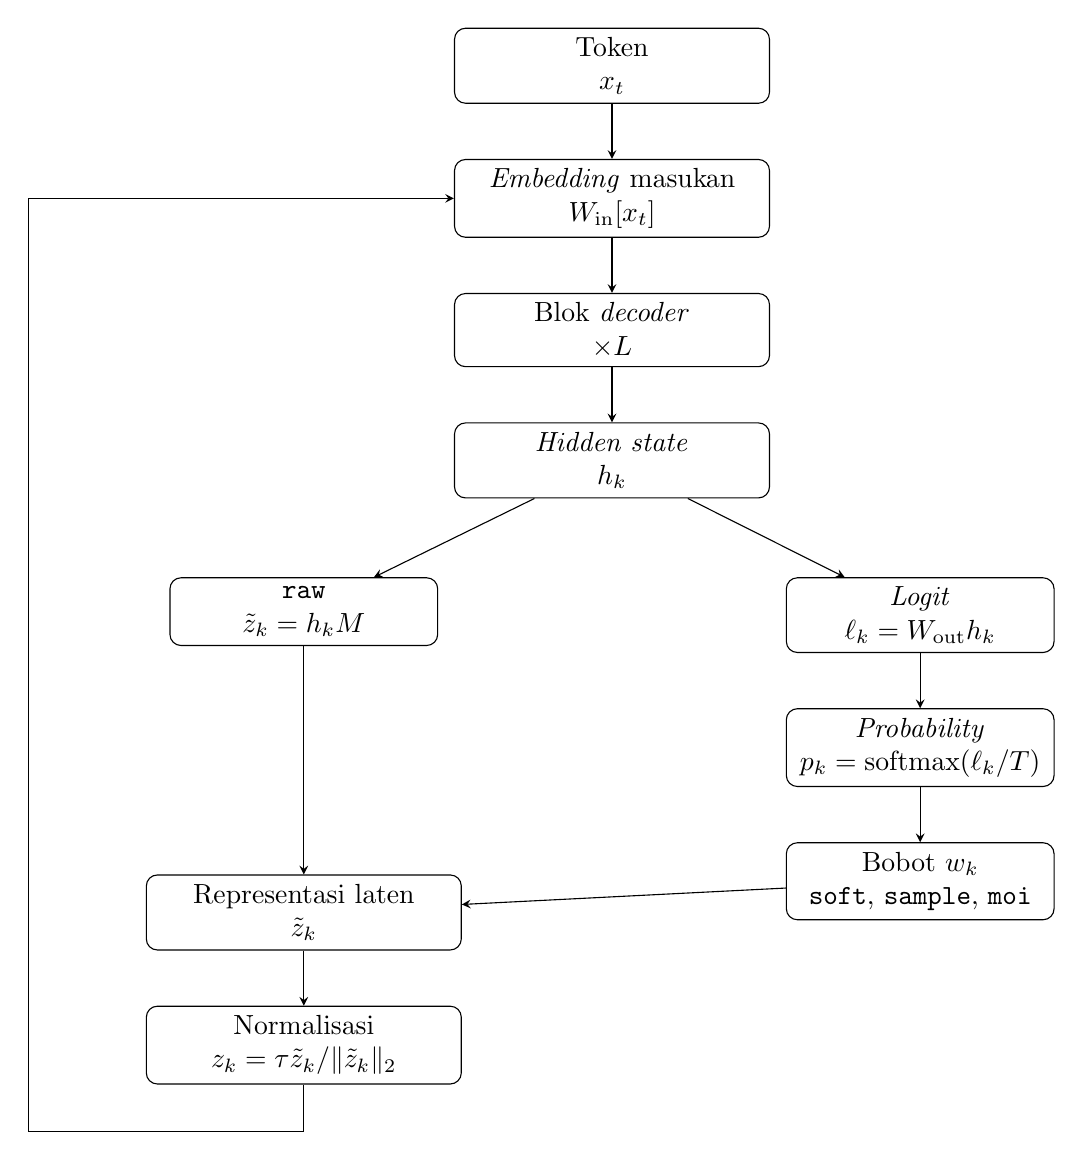
\begin{tikzpicture}[
node distance=7mm,
box/.style={
draw,
rounded corners,
align=center,
minimum width=4.0cm,
minimum height=8mm
},
smallbox/.style={
draw,
rounded corners,
align=center,
minimum width=3.4cm,
minimum height=8mm
},
arrow/.style={->, >=stealth}
]
    \node[box] (token) {Token\\$x_t$};
    \node[box, below=of token] (embed)
    {\textit{Embedding} masukan\\$W_{\mathrm{in}}[x_t]$};
    \node[box, below=of embed] (decoder)
    {Blok \textit{decoder}\\$\times L$};
    \node[box, below=of decoder] (hidden)
    {\textit{Hidden state}\\$h_k$};

    \node[smallbox, below left=10mm and 2mm of hidden] (raw)
        {\code{raw}\\$\tilde{z}_k=h_kM$};

    \node[smallbox, below right=10mm and 2mm of hidden] (logit)
        {\textit{Logit}\\$\ell_k=W_{\mathrm{out}}h_k$};

    \node[smallbox, below=of logit] (prob)
        {\textit{Probability}\\$p_k=\operatorname{softmax}(\ell_k/T)$};

    \node[smallbox, below=of prob] (weight)
        {Bobot $w_k$\\\code{soft}, \code{sample}, \code{moi}};

    \node[box, below=29mm of raw] (latent)
        {Representasi laten\\$\tilde{z}_k$};

    \node[box, below=of latent] (normal)
        {Normalisasi \\$z_k=\tau\tilde{z}_k/\|\tilde{z}_k\|_2$};

    \draw[arrow] (token) -- (embed);
    \draw[arrow] (embed) -- (decoder);
    \draw[arrow] (decoder) -- (hidden);

    \draw[arrow] (hidden) -- (raw);
    \draw[arrow] (hidden) -- (logit);
    \draw[arrow] (logit) -- (prob);
    \draw[arrow] (prob) -- (weight);

    \draw[arrow] (raw) -- (latent);
    \draw[arrow] (weight) -- (latent);

    \draw[arrow] (latent) -- (normal);
    \draw[arrow] (normal.south) -- ++(0, -6mm)
        -- ++(-35mm, 0)
        |- (embed.west);
\end{tikzpicture}
\caption{Alur representasi laten pada arsitektur Qwen3.}
\label{fig:m-latent-overview}

\end{figure}


\subsection{Blok \textit{Decoder}}
\label{subsec:m-decoder}

Masukan bagi lapisan pertama blok \textit{decoder} adalah barisan
vektor \textit{embedding} token. Jika $x_t\in\{1,\ldots,V\}$
menyatakan indeks token pada posisi $t$, maka representasi awal
token tersebut dapat dituliskan sebagai
\begin{equation}
x_t^{(0)}=W_{\mathrm{in}}[x_t],
\label{eq:m-arch-input}
\end{equation}

dengan $W_{\mathrm{in}}\in\mathbb{R}^{V\times d}$
dan $x_t^{(0)}\in\mathbb{R}^{d}$.

Setiap lapisan(\textit{layer}) ke-$l$, untuk $l=1,\ldots,L$, terdiri atas dua
sublapisan, yaitu mekanisme atensi (\textit{attention}) yang
menggabungkan informasi antarposisi dan jaringan umpan-maju
(\textit{feed-forward network}).
Transformasi pada posisi $t$ dapat dituliskan sebagai

\begin{align}
\widetilde{x}_t^{(l)}
&=
x_t^{(l-1)}
+
\operatorname{Attn}^{(l)}
\left(
\operatorname{RMSNorm}
\left(x_t^{(l-1)}\right)
\mid
\mathrm{KV}_{1:t}^{(l)}
\right),
\label{eq:m-arch-attn}
\\[2pt]
x_t^{(l)}
&=
\widetilde{x}_t^{(l)}
+
\operatorname{MLP}^{(l)}
\left(
\operatorname{RMSNorm}
\left(\widetilde{x}_t^{(l)}\right)
\right),
\label{eq:m-arch-mlp}
\end{align}

dengan $x_t^{(l-1)},\widetilde{x}_t^{(l)},x_t^{(l)}
\in\mathbb{R}^{d}$ menyatakan representasi token
pada tahapan yang berbeda. Notasi
$\mathrm{KV}_{1:t}^{(l)}$ menyatakan kumpulan representasi
\textit{key} dan \textit{value} internal pada lapisan ke-$l$
untuk posisi $1,\ldots,t$. Simbol $\mid$ memisahkan masukan
\textit{query} dari kumpulan \textit{key} dan \textit{value}
yang digunakan dalam perhitungan atensi.

Setelah seluruh $L$ lapisan selesai diproses, representasi pada
posisi terakhir dinormalisasi kembali untuk memperoleh
\textit{hidden state} yang digunakan oleh metode laten. Jika
posisi terakhir dinyatakan dengan indeks $T$, maka
\begin{equation}
h_T
=
\operatorname{RMSNorm}\left(x_T^{(L)}\right),
\qquad
h_T\in\mathbb{R}^{d}.
\label{eq:m-arch-h}
\end{equation}

Normalisasi yang digunakan adalah
\textit{Root Mean Square Normalization} (RMSNorm). Untuk suatu
vektor $x\in\mathbb{R}^{d}$, RMSNorm didefinisikan sebagai
\begin{equation}
\operatorname{RMSNorm}(x)
=
\frac{x}{
\sqrt{
\frac{1}{d}\sum_{j=1}^{d}x_j^2+\epsilon
}
}
\odot g,
\qquad
\epsilon=10^{-6},
\label{eq:m-arch-rmsnorm}
\end{equation}
dengan $g\in\mathbb{R}^{d}$ merupakan vektor parameter penguatan
yang dipelajari, $\epsilon$ merupakan konstanta untuk menjaga
stabilitas perhitungan, dan $\odot$ menyatakan perkalian Hadamard.
Dimensi $d$ menyesuaikan dimensi vektor yang dinormalisasi.

Sublapisan umpan-maju(\textit{feed-forward}) menggunakan struktur SwiGLU, yaitu varian
jaringan umpan-maju yang menggabungkan mekanisme gerbang
(\textit{gating}) dengan fungsi aktivasi SiLU. Untuk masukan
$x\in\mathbb{R}^{d}$, transformasinya
didefinisikan sebagai

\begin{equation}
\operatorname{MLP}(x)
=
W_{\mathrm{down}}
\left(
\operatorname{SiLU}(W_gx)
\odot
(W_{\mathrm{up}}x)
\right),
\label{eq:m-arch-swiglu}
\end{equation}

dengan
$W_g,W_{\mathrm{up}}
\in\mathbb{R}^{d_{\mathrm{ff}}\times d}$
merupakan matriks proyeksi dari dimensi model ke dimensi
tersembunyi, sedangkan
$W_{\mathrm{down}}
\in\mathbb{R}^{d\times d_{\mathrm{ff}}}$
merupakan matriks proyeksi kembali ke dimensi model.

Matriks $W_g$ memproyeksikan masukan ke jalur gerbang, sedangkan
$W_{\mathrm{up}}$ memproyeksikan masukan ke jalur informasi.
Keluaran kedua jalur digabungkan melalui perkalian Hadamard,
untuk diproyeksikan kembali melalui $W_{\mathrm{down}}$.

Fungsi SiLU didefinisikan sebagai
\begin{equation}
\operatorname{SiLU}(a)=a\,\sigma(a),
\label{eq:m-arch-silu}
\end{equation}

dengan $a\in\mathbb{R}$ dan
$\sigma(a)=1/(1+\exp(-a))$ merupakan fungsi sigmoid.
Untuk masukan berbentuk vektor, fungsi tersebut diterapkan
pada setiap komponennya secara terpisah.

\subsection{\textit{Grouped-Query Attention} dan RoPE}

\label{subsec:m-gqa}

Sub-lapisan \textit{attention} Qwen3-8B menggunakan \textit{grouped-query attention}
(GQA). Model memiliki $H_q=32$ \textit{query heads} dan
$H_{kv}=8$ pasangan \textit{key-value heads} \citep{qwen3}. Dengan
demikian, beberapa \textit{query heads} berbagi pasangan
\textit{key-value} yang sama.

Dimensi setiap \textit{head} ditentukan oleh

\begin{equation}
d_k
=
\frac{d}{H_q}
=
\frac{4096}{32}
=
128.
\label{eq:m-arch-dk}
\end{equation}

Untuk \textit{query head} ke-$\eta$, dengan
$\eta\in\{1,\ldots,32\}$, indeks pasangan \textit{key-value} yang
digunakan dapat dinyatakan sebagai

\begin{equation}
g(\eta)
=
\left\lceil
\frac{\eta}{H_q/H_{kv}}
\right\rceil
=
\left\lceil
\frac{\eta}{4}
\right\rceil,
\qquad
g(\eta)\in\{1,\ldots,8\}.
\label{eq:m-arch-gqa}
\end{equation}


\begin{figure}[H]
    \centering
    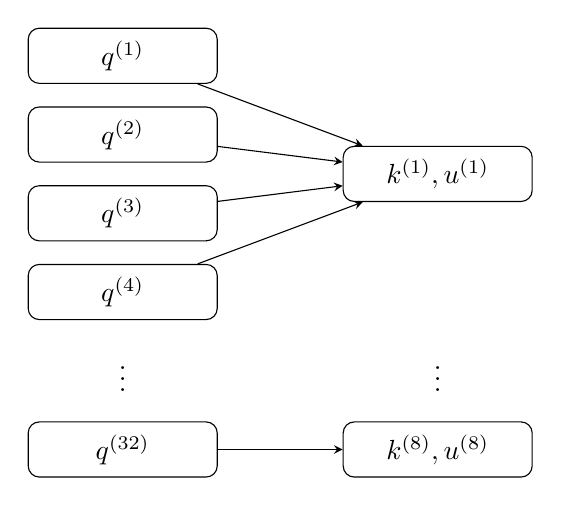
\begin{tikzpicture}[
        box/.style={
            draw,
            rounded corners,
            align=center,
            minimum width=2.4cm,
            minimum height=7mm
        },
        arrow/.style={->, >=stealth}
    ]
        \node[box] (q1) at (0,2.0) {$q^{(1)}$};
        \node[box] (q2) at (0,1.0) {$q^{(2)}$};
        \node[box] (q3) at (0,0.0) {$q^{(3)}$};
        \node[box] (q4) at (0,-1.0) {$q^{(4)}$};

        \node[box] (kv1) at (4,0.5)
            {$k^{(1)},u^{(1)}$};

        \draw[arrow] (q1) -- (kv1);
        \draw[arrow] (q2) -- (kv1);
        \draw[arrow] (q3) -- (kv1);
        \draw[arrow] (q4) -- (kv1);

        \node at (0,-2.0) {$\vdots$};
        \node at (4,-2.0) {$\vdots$};

        \node[box] (q32) at (0,-3.0) {$q^{(32)}$};
        \node[box] (kv8) at (4,-3.0)
            {$k^{(8)},u^{(8)}$};

        \draw[arrow] (q32) -- (kv8);
    \end{tikzpicture}
    \caption{Ilustrasi pembagian \textit{query heads} pada GQA.}
    \label{fig:m-gqa}
\end{figure}


Untuk \textit{query head} ke-$\eta$, \textit{query}, \textit{key}, dan \textit{value} diperoleh melalui proyeksi dari vektor masukan yang telah dinormalisasi, yaitu $x\in\mathbb{R}^{d}$, melalui

\begin{equation}
q^{(\eta)}
=
W_Q^{(\eta)}x,
\qquad
k^{(g(\eta))}
=
W_K^{(g(\eta))}x,
\qquad
v^{(g(\eta))}
=
W_V^{(g(\eta))}x,
\label{eq:m-arch-qku}
\end{equation}

dengan $W_Q^{(\eta)}$, $W_K^{(g(\eta))}$, $W_V^{(g(\eta))}\in\mathbb{R}^{d_k\times d}$
merupakan matriks proyeksi yang dipelajari selama pelatihan dan $q^{(\eta)},k^{(g(\eta))}$, 
$v^{(g(\eta))}\in\mathbb{R}^{d_k}$.

Sebelum digunakan dalam perhitungan \textit{attention}, informasi posisi direpresentasikan menggunakan \textit{Rotary Position Embedding} (RoPE) \citep{roformer}.


\begin{definisi}[Rotary Position Embedding (RoPE)]
\label{def:rope}
Rotary Position Embedding (RoPE) merupakan transformasi yang
merepresentasikan informasi posisi token melalui rotasi pasangan
komponen vektor. Untuk pasangan komponen ke-$r$ pada posisi $t$,
transformasi tersebut didefinisikan sebagai
\begin{equation}
\begin{pmatrix}
x'_{t,2r}\\
x'_{t,2r+1}
\end{pmatrix}
=
\begin{pmatrix}
\cos\theta_{t,r} & -\sin\theta_{t,r}\\
\sin\theta_{t,r} & \cos\theta_{t,r}
\end{pmatrix}
\begin{pmatrix}
x_{t,2r}\\
x_{t,2r+1}
\end{pmatrix},
\label{eq:m-arch-rope}
\end{equation}

dengan $x_{t,2r}$ dan $x_{t,2r+1}$ menyatakan dua komponen
vektor sebelum rotasi, $x'_{t,2r}$ dan $x'_{t,2r+1}$ menyatakan
komponen setelah rotasi, serta $\theta_{t,r}$ menyatakan sudut
rotasi yang bergantung pada posisi $t$ dan indeks pasangan $r$.
Transformasi ini diterapkan pada vektor \textit{query} dan
\textit{key} sebelum perhitungan \textit{attention}.
\end{definisi}

Berdasarkan Definisi~\ref{def:rope}, penerapan RoPE pada
\textit{query} di posisi $i$ dan \textit{key} di posisi $j$
dinyatakan sebagai

\begin{equation}
\begin{aligned}
\widetilde{q}_i^{(\eta)}
&=
\operatorname{RoPE}_i\left(q_i^{(\eta)}\right),\\
\widetilde{k}_j^{(g(\eta))}
&=
\operatorname{RoPE}_j\left(k_j^{(g(\eta))}\right).
\end{aligned}
\label{eq:m-arch-rope-qk}
\end{equation}

dengan $i,j\in\{1,\ldots,L\}$ masing-masing menyatakan posisi
\textit{query} dan \textit{key} dalam urutan sepanjang $L$ token,
serta $q_i^{(\eta)},\widetilde{q}_i^{(\eta)},
k_j^{(g(\eta))},\widetilde{k}_j^{(g(\eta))}
\in\mathbb{R}^{d_k}$ merupakan vektor \textit{query} dan
\textit{key} sebelum dan sesudah penerapan RoPE.

Vektor hasil rotasi tersebut digunakan untuk menghitung skor
kesesuaian antara \textit{query} dan \textit{key} yang dinormalisasi
untuk menghasilkan bobot \textit{attention}. Untuk posisi
\textit{query} $i$ dan posisi \textit{key} $j$, bobot
\textit{attention} dapat dituliskan sebagai
\begin{equation}
\begin{gathered}
\alpha_{ij}^{(\eta)}
=
\frac{
\exp\left(
\frac{
\left(\widetilde{q}_i^{(\eta)}\right)^{\mathsf T}
\widetilde{k}_j^{(g(\eta))}
}{
\sqrt{d_k}
}
\right)
}{
\displaystyle
\sum_{r=1}^{i}
\exp\left(
\frac{
\left(\widetilde{q}_i^{(\eta)}\right)^{\mathsf T}
\widetilde{k}_r^{(g(\eta))}
}{
\sqrt{d_k}
}
\right)
},
\\[6pt]
\alpha_{ij}^{(\eta)}\geq 0,
\qquad
\sum_{j=1}^{i}\alpha_{ij}^{(\eta)}=1.
\end{gathered}
\label{eq:m-arch-attention-weight}
\end{equation}
dengan $r$ merupakan indeks penjumlahan posisi \textit{key}
yang berjalan dari $1$ hingga $i$,
$\alpha_{ij}^{(\eta)}\in[0,1]$ merupakan bobot skalar
\textit{attention} antara \textit{query} pada posisi $i$
dan \textit{key} pada posisi $j$.

Bobot $\alpha_{ij}^{(\eta)}$ selanjutnya digunakan untuk
menggabungkan vektor \textit{value} pada posisi-posisi yang
dapat diakses oleh \textit{query}. Keluaran \textit{attention}
untuk \textit{query head} ke-$\eta$ pada posisi $i$ dapat
dituliskan sebagai
\begin{equation}
o_i^{(\eta)}
=
\sum_{j=1}^{i}
\alpha_{ij}^{(\eta)}
u_j^{(g(\eta))},
\qquad
o_i^{(\eta)}\in\mathbb{R}^{d_k}.
\label{eq:m-arch-attention-output}
\end{equation}
dengan $u_j^{(g(\eta))}\in\mathbb{R}^{d_k}$ merupakan vektor
\textit{value} pada posisi $j$ untuk \textit{key-value head}
ke-$g(\eta)$, sedangkan $o_i^{(\eta)}$ merupakan hasil
penjumlahan bobot \textit{attention} dengan vektor \textit{value}.

Persamaan tersebut memperlihatkan bahwa RoPE memengaruhi perhitungan
kesesuaian antara \textit{query} dan \textit{key}, sedangkan vektor
\textit{value} digunakan untuk membentuk keluaran \textit{attention}. Sehingga
\textit{KV-cache} dapat digunakan untuk mempertahankan informasi token
dari posisi-posisi sebelumnya.

\subsection{\textit{KV-cache} per Lapisan}

\label{subsec:m-kvcache}

Pada \textit{Transformer decoder-only}, hasil proyeksi \textit{key} dan
\textit{value} dari posisi-posisi sebelumnya dapat disimpan sehingga tidak
perlu dihitung ulang ketika posisi baru diproses. Penyimpanan tersebut
disebut \textit{KV-cache}.

Untuk lapisan ke-$l$, setelah $t$ posisi diproses,
\textit{KV-cache} secara konseptual dapat dituliskan sebagai

\begin{equation}
\mathrm{KV}^{(l)}_t
=
\left\{
\left(
k_j^{(l,g)},
v_j^{(l,g)}
\right)
:
1\leq j\leq t,\;
1\leq g\leq H_{kv}
\right\}.
\label{eq:m-arch-kv}
\end{equation}

Karena Qwen3-8B memiliki $H_{kv}=8$, setiap posisi baru yang diproses
menambahkan delapan pasangan \textit{key-value} ke dalam \textit{cache}
pada masing-masing lapisan. Secara konseptual, pertumbuhan tersebut
dapat dituliskan sebagai

\begin{equation}
\mathrm{KV}^{(l)}_{t+1}
=
\mathrm{KV}^{(l)}_t
\;\Vert\;
\left\{
\left(
k_{t+1}^{(l,g)},
v_{t+1}^{(l,g)}
\right)
:
1\leq g\leq 8
\right\},
\label{eq:m-arch-kvtumbuh}
\end{equation}

dengan $\Vert$ menyatakan penggabungan sepanjang dimensi posisi.

\begin{figure}[H]
    \centering
    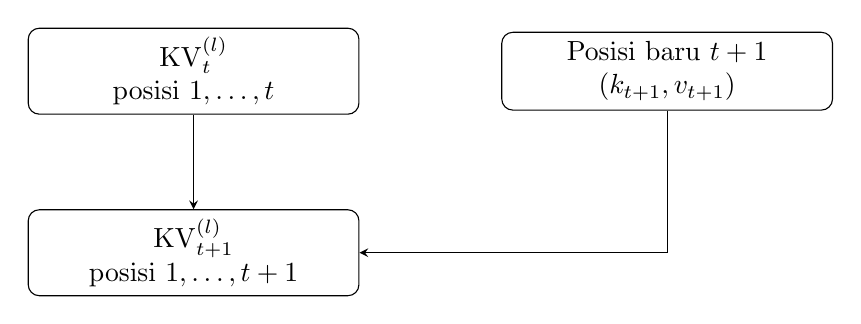
\begin{tikzpicture}[
        box/.style={
            draw,
            rounded corners,
            align=center,
            minimum width=4.2cm,
            minimum height=8mm
        },
        arrow/.style={->, >=stealth}
    ]
        \node[box] (old) {$\mathrm{KV}^{(l)}_t$\\
        posisi $1,\ldots,t$};

        \node[box, right=18mm of old] (new)
            {Posisi baru $t+1$\\
            $(k_{t+1},v_{t+1})$};

        \node[box, below=12mm of old] (updated)
            {$\mathrm{KV}^{(l)}_{t+1}$\\
            posisi $1,\ldots,t+1$};

        \draw[arrow] (old) -- (updated);
        \draw[arrow] (new) |- (updated);
    \end{tikzpicture}
    \caption{Pertumbuhan \textit{KV-cache} ketika posisi baru diproses.}
    \label{fig:m-kvcache}
\end{figure}

Sifat pertumbuhan \textit{KV-cache} tersebut penting dalam penelitian ini
karena sebuah vektor pada langkah laten juga diproses sebagai posisi baru.
Oleh sebab itu, langkah laten tidak hanya menghasilkan \textit{hidden
state} baru, tetapi juga memperbarui \textit{KV-cache}. Dalam sistem
multi-agen, \textit{KV-cache} inilah yang digunakan sebagai salah satu
medium komunikasi antar-agen.

\subsection{\textit{Embedding} Masukan dan Keluaran}

\label{subsec:m-embedding}

Qwen3-8B menggunakan matriks \textit{embedding} masukan dan matriks
keluaran yang tidak diikat (\textit{untied embedding}) \citep{qwen3}.
Konvensi kolom yang digunakan dalam penelitian ini dapat
dituliskan sebagai

\begin{equation}
W_{\mathrm{in}},
\;
W_{\mathrm{out}}
\in
\mathbb{R}^{V\times d}.
\label{eq:m-arch-embedding}
\end{equation}

Matriks $W_{\mathrm{in}}$ digunakan untuk memperoleh vektor
\textit{embedding} token. Jika $x_t$ merupakan indeks token, maka

\begin{equation}
x_t^{(0)}
=
W_{\mathrm{in}}[x_t].
\label{eq:m-arch-win}
\end{equation}

Sebaliknya, matriks $W_{\mathrm{out}}$ digunakan untuk mengubah
\textit{hidden state} menjadi \textit{logit}. Untuk suatu
$h\in\mathbb{R}^{d}$, diperoleh

\begin{equation}
\ell
=
W_{\mathrm{out}}h,
\label{eq:m-arch-logit}
\end{equation}

dengan $\ell\in\mathbb{R}^{V}$ merupakan vektor \textit{logit} untuk
seluruh entri kosakata. Ukuran kosakata yang sesuai dengan jumlah baris kedua matriks tersebut
adalah $V = 151\,936$.

\begin{figure}[H]
    \centering
    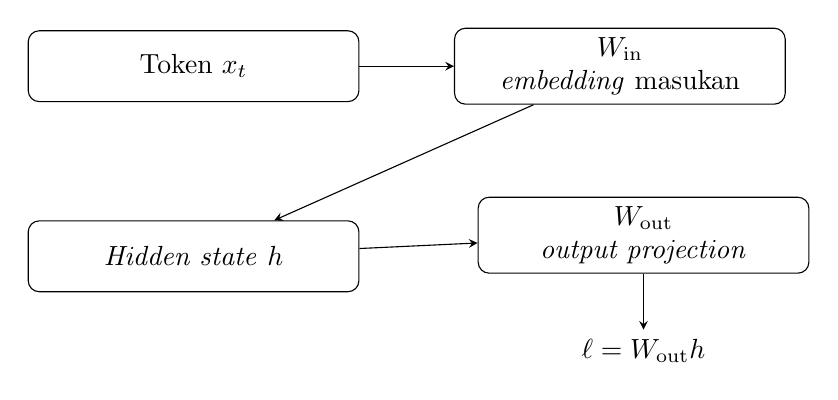
\begin{tikzpicture}[
        box/.style={
            draw,
            rounded corners,
            align=center,
            minimum width=4.2cm,
            minimum height=9mm
        },
        arrow/.style={->, >=stealth}
    ]
        \node[box] (token) {Token $x_t$};
        \node[box, right=12mm of token] (win)
            {$W_{\mathrm{in}}$\\
            \textit{embedding} masukan};
        \node[box, below right=12mm and 15mm of token] (wout)
            {$W_{\mathrm{out}}$\\
            \textit{output projection}};

        \node[box, below=15mm of token] (hidden)
            {\textit{Hidden state} $h$};

        \draw[arrow] (token) -- (win);
        \draw[arrow] (win) -- (hidden);
        \draw[arrow] (hidden) -- (wout);
        \draw[arrow] (wout) -- ++(0,-12mm)
            node[below] {$\ell=W_{\mathrm{out}}h$};
    \end{tikzpicture}
    \caption{Hubungan \textit{embedding} masukan dan keluaran pada Qwen3-8B.}
    \label{fig:m-embedding}
\end{figure}


Karena kedua matriks tidak diikat, $W_{\mathrm{in}}$ dan
$W_{\mathrm{out}}$ merupakan parameter yang dipelajari secara independen.
Pada model yang digunakan dalam penelitian ini, rata-rata kosinus antara
baris yang bersesuaian dari kedua matriks diukur sebesar

\begin{equation}
\frac{1}{V}
\sum_{i=1}^{V}
\cos
\left(
W_{\mathrm{in}}[i],
W_{\mathrm{out}}[i]
\right)
=
0{,}0041.
\label{eq:m-arch-cos}
\end{equation}

Nilai tersebut merupakan hasil pengukuran pada bobot model yang digunakan,
bukan parameter arsitektur Qwen3. Hasil ini menunjukkan bahwa pasangan
baris yang bersesuaian antara $W_{\mathrm{in}}$ dan $W_{\mathrm{out}}$
tidak memiliki keselarasan arah yang kuat. Hal tersebut menjadi relevan
bagi metode \code{raw}, karena \textit{hidden state} keluaran perlu
diselaraskan terlebih dahulu sebelum digunakan sebagai vektor pada ruang
\textit{embedding} masukan.

Parameter arsitektur yang digunakan dalam penelitian ini dirangkum pada
Tabel~\ref{tab:m-arsitektur}.

\begin{table}[H]
    \centering
    \caption{Parameter arsitektur Qwen3-8B yang digunakan dalam penelitian.}
    \label{tab:m-arsitektur}
    \small
    \begin{tabular}{lll}
        \hline
        Komponen & Nilai & Sumber \\
        \hline
        Jumlah lapisan $L$ & $36$ & \citet{qwen3} \\
        Dimensi \textit{hidden state} $d$ & $4096$ & \citet{qwen3} \\
        \textit{Query heads} $H_q$ & $32$ & \citet{qwen3} \\
        \textit{Key-value heads} $H_{kv}$ & $8$ & \citet{qwen3} \\
        Dimensi tiap \textit{head} $d_k$ & $128$ & $d/H_q$ \\
        Ukuran kosakata $V$ & $151\,936$ & pengukuran model \\
        \textit{Embedding} & \textit{untied} & \citet{qwen3} \\
        Rata-rata kosinus per baris & $0{,}0041$ & pengukuran model \\
        Normalisasi & RMSNorm, \textit{pre-norm} & \citet{qwen3} \\
        \textit{feed-forward} & SwiGLU & \citet{qwen3} \\
        Representasi posisi & RoPE & \citet{qwen3} \\
        \hline
    \end{tabular}
\end{table}

%==========================================================================
\section{Langkah Laten dalam Satu Agen}

\label{sec:langkah-laten}

Langkah laten merupakan mekanisme yang memungkinkan model melakukan \textit{reasoning} 
tanpa menghasilkan token diskret. Pada generasi autoregresif konvensional, \textit{hidden
state} pada suatu posisi diproyeksikan ke ruang kosakata untuk menghasilkan
distribusi token berikutnya. Satu token kemudian dipilih dari distribusi tersebut
dan \textit{embedding} token yang terpilih digunakan sebagai masukan pada
langkah berikutnya. Dengan demikian, informasi yang diteruskan ke langkah
berikutnya direpresentasikan oleh satu token diskret.

Pada penelitian ini, representasi tersebut digantikan oleh vektor laten
$z_k\in\mathbb{R}^{d}$ yang diberikan langsung kepada model melalui
\textit{input embedding} pada langkah berikutnya. Vektor laten tidak didekode
menjadi token selama proses ini, tetapi diproses kembali oleh model untuk
menghasilkan \textit{hidden state} baru dan memperbarui \textit{key-value
cache} (KV cache). Dengan demikian, langkah laten membentuk suatu proses
iteratif pada ruang representasi kontinu.

\begin{figure}[htbp]
    \centering
    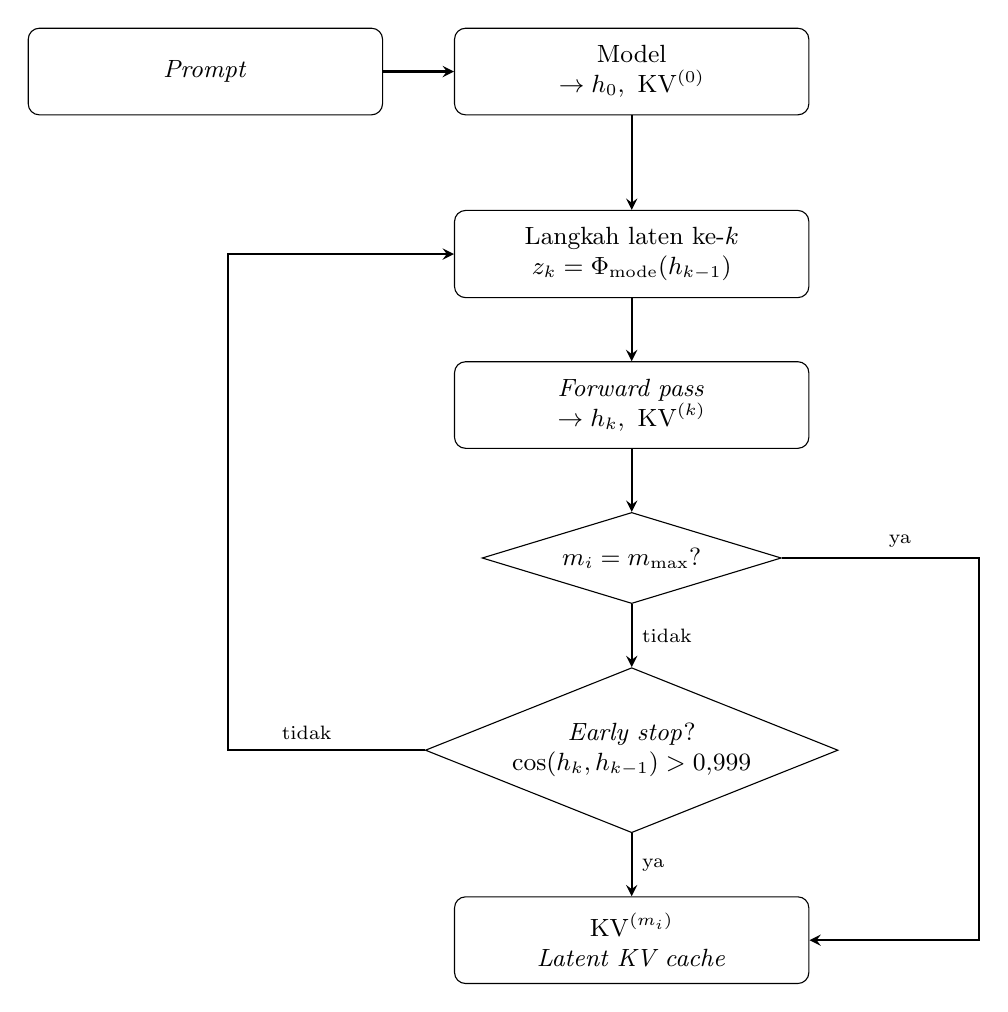
\begin{tikzpicture}[
        node distance=0.8cm and 0.9cm,
        every node/.style={align=center, font=\small},
        box/.style={
            draw,
            rounded corners,
            inner sep=6pt,
            minimum width=4.5cm,
            minimum height=1.1cm
        },
        decision/.style={
            draw,
            diamond,
            aspect=2.5,
            inner sep=2pt,
            align=center,
            minimum width=3.8cm
        },
        arrow/.style={->, >=stealth, thick}
    ]

    \node[box] (prompt) {\textit{Prompt}};

    \node[box, right=of prompt] (model)
        {Model\\$ \to h_0,\ \mathrm{KV}^{(0)} $};

    \node[box, below=12mm of model] (latent)
        {Langkah laten ke-$k$\\
        $z_k=\Phi_{\mathrm{mode}}(h_{k-1})$};

    \node[box, below=of latent] (forward)
        {\textit{Forward pass}\\
        $\to h_k,\ \mathrm{KV}^{(k)}$};

    \node[decision, below=of forward] (check)
        {$m_i=m_{\max}$?};

    \node[decision, below=of check] (early)
        {\textit{Early stop}?\\
        $\cos(h_k,h_{k-1})>0{,}999$};

    \node[box, below=of early] (kv)
        {$\mathrm{KV}^{(m_i)}$\\
        \textit{Latent KV cache}};

    \draw[arrow] (prompt) -- (model);
    \draw[arrow] (model) -- (latent);
    \draw[arrow] (latent) -- (forward);
    \draw[arrow] (forward) -- (check);

    \draw[arrow]
        (check)
        -- node[right, font=\scriptsize] {tidak}
        (early);

    \draw[arrow]
        (early)
        -- node[right, font=\scriptsize] {ya}
        (kv);

    \draw[arrow]
        (check.east)
        -- ++(2.5cm,0)
        node[above, font=\scriptsize, pos=0.6] {ya}
        |- (kv.east);

    \draw[arrow]
        (early.west)
        -- ++(-2.5cm,0)
        node[above, font=\scriptsize, pos=0.6] {tidak}
        |- (latent.west);

    \end{tikzpicture}
    \caption{Alur satu \textit{latent pass} pada satu agen.}
    \label{fig:one-latent-pass}
\end{figure}

\subsection{Satu \textit{Latent Pass}}

\label{subsec:one-latent-pass}

Satu agen menjalankan sejumlah langkah laten secara berurutan dalam satu
\textit{latent pass}. Proses dimulai dengan pemrosesan \textit{prompt} oleh
model hingga diperoleh \textit{hidden state} awal $h_0$ dan
\textit{key-value cache} (KV cache) awal $\mathrm{KV}^{(0)}$. Selanjutnya,
\textit{hidden state} digunakan untuk membentuk vektor laten, yang kemudian
diberikan kembali kepada model sebagai masukan pada langkah berikutnya.
Secara konseptual, inisialisasi tersebut dapat dituliskan sebagai

\begin{equation}
    \mathrm{Prompt}
    \longrightarrow
    \left(
        h_0,\mathrm{KV}^{(0)}
    \right).
    \label{eq:latent-pass-init}
\end{equation}

Untuk setiap langkah ke-$k$, vektor laten dibentuk dari
\textit{hidden state} sebelumnya dan kemudian diproses kembali oleh model,
sehingga

\begin{equation}
    z_k
    =
    \Phi_{\mathrm{mode}}(h_{k-1}),
    \label{eq:latent-pass-z}
\end{equation}

\begin{equation}
    \left(
        h_k,\mathrm{KV}^{(k)}
    \right)
    =
    f_{\theta}
    \left(
        z_k,
        \mathrm{KV}^{(k-1)}
    \right),
    \label{eq:latent-pass-forward}
\end{equation}

dengan $h_{k-1}\in\mathbb{R}^{d}$ merupakan \textit{hidden state} sebelum
langkah laten ke-$k$, $z_k\in\mathbb{R}^{d}$ merupakan vektor laten yang
diberikan kembali kepada model, $\Phi_{\mathrm{mode}}$ merupakan fungsi
pembentukan vektor laten yang bergantung pada metode, dan $f_{\theta}$
menyatakan satu \textit{forward pass} model dengan \textit{KV cache} yang
telah terbentuk sebelumnya.

Dengan demikian, rangkaian langkah laten dalam satu \textit{latent pass}
dapat dinyatakan sebagai

\begin{equation}
    h_0
    \longrightarrow
    z_1
    \longrightarrow
    h_1
    \longrightarrow
    z_2
    \longrightarrow
    \cdots
    \longrightarrow
    z_{m_i}
    \longrightarrow
    h_{m_i}.
    \label{eq:latent-iteration}
\end{equation}

Pada setiap langkah, vektor $z_k$ tidak didekode menjadi token diskret,
melainkan langsung digunakan sebagai masukan kontinu melalui
\textit{input embedding}. Oleh karena itu, rangkaian tersebut merupakan
proses iteratif pada ruang representasi kontinu.

Selain menghasilkan \textit{hidden state} baru, pemrosesan $z_k$ juga
memperbarui \textit{KV cache}. Pada lapisan ke-$l$, \textit{KV cache} setelah
$t$ posisi dapat direpresentasikan sebagai

\begin{equation}
    \mathrm{KV}^{(l)}_t
    =
    \left\{
        \left(
            k^{(l)}_j,
            v^{(l)}_j
        \right)
    \right\}_{j=1}^{t},
    \label{eq:kv-cache-definition}
\end{equation}

dengan $k^{(l)}_j$ dan $v^{(l)}_j$ masing-masing merupakan vektor
\textit{key} dan \textit{value} pada posisi ke-$j$ di lapisan ke-$l$.
Secara konseptual, ketika $z_k$ diproses oleh model, \textit{KV cache}
diperbarui melalui

\begin{equation}
    \mathrm{KV}^{(k)}
    =
    \mathrm{KV}^{(k-1)}
    \mathbin{\Vert}
    \mathrm{KV}(z_k),
    \label{eq:kv-latent-update}
\end{equation}

dengan $\mathbin{\Vert}$ menyatakan penggabungan sepanjang dimensi
urutan dan $\mathrm{KV}(z_k)$ menyatakan pasangan \textit{key-value} yang
dihasilkan dari pemrosesan $z_k$. Dengan demikian, yang disimpan dalam
\textit{KV cache} bukanlah vektor laten $z_k$ secara langsung, melainkan
representasi \textit{key} dan \textit{value} yang dihasilkan model dari
vektor tersebut.

Setelah seluruh langkah laten selesai, satu \textit{latent pass} menghasilkan
rangkaian vektor laten

\begin{equation}
    Z_i
    =
    \left(
        z_1,\ldots,z_{m_i}
    \right),
    \label{eq:latent-sequence}
\end{equation}

serta \textit{KV cache} akhir

\begin{equation}
    \mathrm{KV}_i
    =
    \mathrm{KV}^{(m_i)}.
    \label{eq:latent-kv-final}
\end{equation}

Pada mode komunikasi yang menghasilkan keluaran teks, \textit{KV cache}
akhir tersebut selanjutnya digunakan sebagai konteks untuk proses generasi
teks. Dengan demikian, generasi teks merupakan tahap setelah
\textit{latent pass}, sedangkan pengulangan langkah laten berlangsung
sepenuhnya sebelum tahap tersebut.

\subsection{\textit{Early Stopping} pada Langkah Laten}

\label{subsec:latent-early-stopping}

Jumlah langkah laten maksimum pada penelitian ini ditetapkan sebesar
$m_{\max}=10$. Namun, satu agen tidak selalu menjalankan seluruh langkah
tersebut. Setelah \textit{hidden state} baru $h_k$ diperoleh, kemiripannya
dengan \textit{hidden state} pada langkah sebelumnya $h_{k-1}$ digunakan
sebagai kriteria untuk menentukan apakah proses laten masih perlu
dilanjutkan.

Kemiripan tersebut diukur menggunakan \textit{cosine similarity}, yaitu

\begin{equation}
    \operatorname{cos}(h_k,h_{k-1})
    =
    \frac{
        h_k^{\mathsf T}h_{k-1}
    }{
        \left\|h_k\right\|_2
        \left\|h_{k-1}\right\|_2
    }.
    \label{eq:latent-cosine}
\end{equation}

Proses langkah laten dihentikan apabila

\begin{equation}
    \operatorname{cos}(h_k,h_{k-1})
    >
    0{,}999.
    \label{eq:early-stop}
\end{equation}

Kriteria tersebut menunjukkan bahwa proses laten dihentikan ketika dua
\textit{hidden state} berturut-turut memiliki arah yang sangat serupa.
Apabila kriteria tersebut belum terpenuhi, proses dilanjutkan ke langkah
laten berikutnya hingga mencapai batas maksimum.

Dengan demikian, jumlah langkah laten aktual yang dilakukan oleh agen
ke-$i$ memenuhi

\begin{equation}
    1
    \leq
    m_i
    \leq
    m_{\max},
    \qquad
    m_{\max}=10,
    \label{eq:actual-latent-steps}
\end{equation}

dengan $m_i$ ditentukan oleh tercapainya kriteria \textit{early stopping}
atau batas maksimum langkah laten.

\subsection{Dari \textit{Hidden State} ke Distribusi Token}

\label{subsec:hidden-state-distribusi}

Untuk metode yang memanfaatkan distribusi token, $h_k$ terlebih dahulu
diproyeksikan ke ruang kosakata menggunakan matriks keluaran model
$W_{\mathrm{out}}$. Logit token ke-$i$ pada langkah ke-$k$ didefinisikan sebagai

\begin{equation}
\ell_{k,i}
=
W_{\mathrm{out}}[i]^{\mathsf T}h_k,
\label{eq:latent-logit-component}
\end{equation}

atau dalam bentuk vektor,

\begin{equation}
\boldsymbol{\ell}_k
=
W_{\mathrm{out}}h_k
\in
\mathbb{R}^{|\mathcal{V}|}.
\label{eq:latent-logit}
\end{equation}

Selanjutnya, logit tersebut diubah menjadi distribusi probabilitas atas seluruh
kosakata menggunakan fungsi \textit{softmax}. Dengan temperatur $T>0$,
diperoleh

\begin{equation}
p_{k,i}
=
\frac{
\exp\left(\ell_{k,i}/T\right)
}{
\displaystyle
\sum_{j=1}^{|\mathcal{V}|}
\exp\left(\ell_{k,j}/T\right)
},
\qquad
i=1,\ldots,|\mathcal{V}|.
\label{eq:latent-softmax}
\end{equation}

Dalam bentuk vektor, Persamaan~\eqref{eq:latent-softmax} dapat dituliskan
sebagai

\begin{equation}
p_k
=
\operatorname{softmax}
\left(
\frac{\boldsymbol{\ell}_k}{T}
\right)
\in
\Delta^{|\mathcal{V}|-1},
\label{eq:latent-probability}
\end{equation}

dengan

\begin{equation}
\Delta^{|\mathcal{V}|-1}
=
\left\{
w\in\mathbb{R}^{|\mathcal{V}|}
:
w_i\geq0,
\;
\sum_{i=1}^{|\mathcal{V}|}w_i=1
\right\}
\label{eq:probability-simplex}
\end{equation}

merupakan \textit{probability simplex}. Temperatur pada penelitian ini
ditetapkan sebesar

\begin{equation}
T=0{,}7.
\label{eq:latent-temperature}
\end{equation}

Distribusi $p_k$ merupakan distribusi prediktif model terhadap token berikutnya.
Distribusi tersebut menjadi dasar pembentukan bobot $w_k$ pada metode
\texttt{soft}, \texttt{sample}, dan \texttt{moi}. Sebaliknya, metode
\texttt{raw} tidak memerlukan pembentukan distribusi token sehingga tidak
melalui tahapan pada Persamaan~\eqref{eq:latent-logit} hingga
Persamaan~\eqref{eq:latent-probability}.

\subsection{Kerangka Penyatuan Metode}

\label{subsec:kerangka-penyatuan}

Keempat metode pembentukan langkah laten menggunakan \textit{hidden state}
$h_k$ yang sama sebagai sumber informasi. Perbedaan antarmetode terletak pada
mekanisme yang digunakan untuk mengubah \textit{hidden state} tersebut menjadi
representasi laten sebelum diberikan kembali kepada model. Untuk menyatakan
mekanisme tersebut secara umum, digunakan $\Phi_{\mathrm{mode}}$, dengan
$\mathrm{mode}$ menyatakan metode pembentukan representasi laten.

Secara umum, representasi laten dapat dipandang sebagai proses dua tahap.
Tahap pertama menghasilkan representasi laten awal
$\tilde{z}_k^{\mathrm{mode}}$, sedangkan tahap kedua menyesuaikan magnitudonya
agar berada pada skala yang sama untuk seluruh metode. Dengan demikian,

\begin{equation}
    z_k^{\mathrm{mode}}
    =
    \mathcal{N}
    \left(
        \tilde{z}_k^{\mathrm{mode}}
    \right),
    \label{eq:unified-latent-map}
\end{equation}

dengan $\mathcal{N}(\cdot)$ menyatakan operator normalisasi dan
$\tilde{z}_k^{\mathrm{mode}}\in\mathbb{R}^{d}$ merupakan representasi laten
sebelum normalisasi. Normalisasi tersebut didefinisikan sebagai

\begin{equation}
    z_k^{\mathrm{mode}}
    =
    \tau
    \frac{
        \tilde{z}_k^{\mathrm{mode}}
    }{
        \left\|
            \tilde{z}_k^{\mathrm{mode}}
        \right\|_2
    },
    \qquad
    \mathrm{mode}
    \in
    \{
        \mathrm{soft},
        \mathrm{sample},
        \mathrm{moi},
        \mathrm{raw}
    \},
    \label{eq:unified-latent-normalized}
\end{equation}

dengan $\tau>0$ merupakan norma target yang ditetapkan sama untuk seluruh
metode. Dengan normalisasi tersebut, setiap representasi laten yang diberikan
kepada model memenuhi

\begin{equation}
    \left\|
        z_k^{\mathrm{mode}}
    \right\|_2
    =
    \tau.
    \label{eq:unified-latent-norm}
\end{equation}

Sehinggap perbandingan metode selanjutnya bisa berfokus pada mekanisme pembentukan arah
representasi $\tilde{z}_k^{\mathrm{mode}}$.

Untuk metode \texttt{soft}, \texttt{sample}, dan \texttt{moi}, representasi
laten awal dibentuk melalui ruang \textit{input embedding}. Matriks
\textit{input embedding} didefinisikan sebagai

\begin{equation}
    W_{\mathrm{in}}
    =
    \begin{bmatrix}
        W_{\mathrm{in}}[1]^{\mathsf T}\\
        \vdots\\
        W_{\mathrm{in}}[|\mathcal{V}|]^{\mathsf T}
    \end{bmatrix}
    \in
    \mathbb{R}^{|\mathcal{V}|\times d},
    \label{eq:input-embedding-matrix}
\end{equation}

dengan $W_{\mathrm{in}}[i]\in\mathbb{R}^{d}$ merupakan vektor
\textit{embedding} token ke-$i$. Apabila $w_k$ menyatakan bobot atas kosakata,
maka representasi laten awal dapat dituliskan secara umum sebagai

\begin{equation}
    \tilde{z}_k^{\mathrm{mode}}
    =
    W_{\mathrm{in}}^{\mathsf T}w_k,
    \qquad
    \mathrm{mode}
    \in
    \{
        \mathrm{soft},
        \mathrm{sample},
        \mathrm{moi}
    \}.
    \label{eq:unified-latent-pre}
\end{equation}

Karena $w_k$ merupakan bobot atas kosakata, bentuk tersebut mencakup
pembentukan representasi melalui kombinasi berbobot dari vektor
\textit{embedding}. Perbedaan antara \texttt{soft}, \texttt{sample}, dan
\texttt{moi} dengan demikian tidak terletak pada bentuk pemetaan
$W_{\mathrm{in}}^{\mathsf T}w_k$, tetapi pada cara masing-masing metode
memperoleh $w_k$.

Sementara itu, metode \texttt{raw} tidak membentuk representasi melalui
bobot atas kosakata. Metode ini memetakan \textit{hidden state} secara langsung
ke ruang \textit{input embedding} menggunakan matriks penyelarasan
$M\in\mathbb{R}^{d\times d}$, sehingga

\begin{equation}
    \tilde{z}_k^{\mathrm{raw}}
    =
    M^{\mathsf T}h_k.
    \label{eq:raw-pre-normalization}
\end{equation}

Dengan demikian, keempat metode dapat ditempatkan dalam satu kerangka umum,
yaitu

\begin{equation}
    h_k
    \longrightarrow
    \tilde{z}_k^{\mathrm{mode}}
    \longrightarrow
    z_k^{\mathrm{mode}},
    \label{eq:latent-flow-unified}
\end{equation}

dengan perbedaan antarmetode ditentukan oleh pemetaan yang menghasilkan
$\tilde{z}_k^{\mathrm{mode}}$. Untuk \texttt{soft}, \texttt{sample}, dan
\texttt{moi}, pemetaan tersebut melalui bobot atas kosakata, sedangkan
\texttt{raw} menggunakan pemetaan langsung dari \textit{hidden state}.



%=================================================================================


\section{Mixture of Inputs}

\label{subsec:mixture-of-inputs}

Pada langkah laten, \textit{hidden state} $h_k$ terlebih dahulu digunakan untuk menghasilkan distribusi probabilitas token berikutnya. Pada metode \textit{Mixture of Inputs} (MoI), distribusi tersebut tidak langsung direduksi menjadi satu token, tetapi digunakan bersama dengan token hasil \textit{sampling} untuk membentuk bobot campuran yang kemudian digunakan dalam penyusunan representasi masukan berikutnya. Dengan demikian, informasi mengenai ketidakpastian model tetap dipertahankan pada representasi kontinu yang diberikan kembali kepada model.

Secara umum, alur pembentukan representasi laten pada metode MoI dapat dituliskan sebagai berikut.

\begin{figure}[H]
\centering
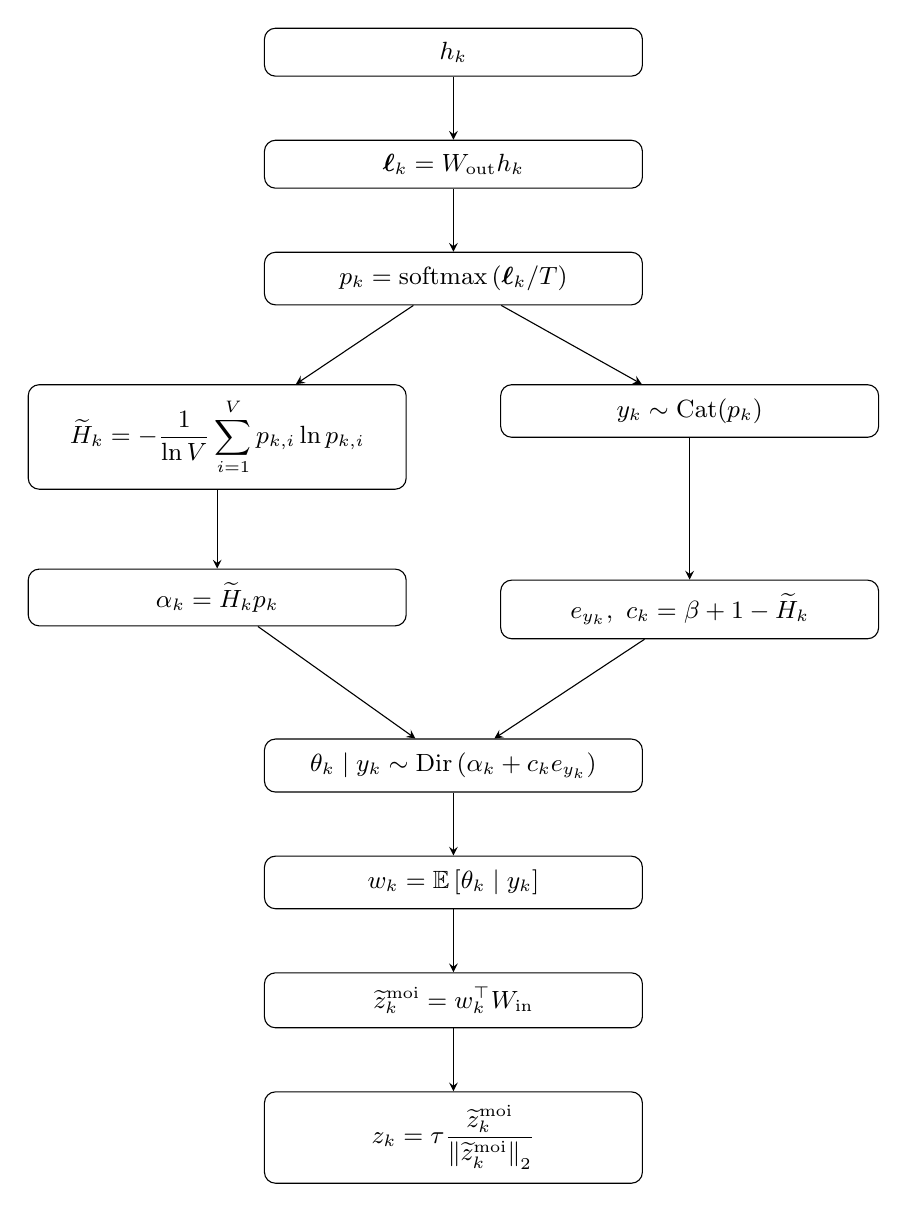
\begin{tikzpicture}[
    node distance=8mm,
    every node/.style={
        align=center,
        font=\small
    },
    box/.style={
        draw,
        rounded corners,
        inner sep=5pt,
        minimum width=4.8cm
    },
    arrow/.style={
        ->,
        >=stealth
    }
]

\node[box] (h) {$h_k$};

\node[box, below=of h] (logits)
    {$\boldsymbol{\ell}_k = W_{\mathrm{out}}h_k$};

\node[box, below=of logits] (prob)
    {$p_k=\operatorname{softmax}
    \left(\boldsymbol{\ell}_k/T\right)$};

\node[box, below=10mm of prob, xshift=-3cm] (entropy)
    {$\widetilde H_k
    =
    -\dfrac{1}{\ln V}
    \displaystyle\sum_{i=1}^{V}
    p_{k,i}\ln p_{k,i}$};
    
\node[box, below=10mm of prob, xshift=3cm] (sample)
    {$y_k\sim\operatorname{Cat}(p_k)$};

\node[box, below=10mm of entropy] (alpha)
    {$\alpha_k=\widetilde H_k p_k$};

\node[box, below=18mm of sample] (obs)
    {$e_{y_k},\ c_k=\beta+1-\widetilde H_k$};

\node[box, below=5.5cm of prob] (posterior)
    {$\theta_k\mid y_k
    \sim
    \operatorname{Dir}
    \left(
    \alpha_k+c_k e_{y_k}
    \right)$};

\node[box, below=of posterior] (weight)
    {$w_k=\mathbb{E}
    \left[\theta_k\mid y_k\right]$};

\node[box, below=of weight] (latent)
    {$\widetilde z_k^{\mathrm{moi}}
    =
    w_k^{\top}W_{\mathrm{in}}$};

\node[box, below=of latent] (norm)
    {$z_k
    =
    \tau
    \dfrac{
    \widetilde z_k^{\mathrm{moi}}
    }{
    \left\|
    \widetilde z_k^{\mathrm{moi}}
    \right\|_2
    }$};

\draw[arrow] (h) -- (logits);
\draw[arrow] (logits) -- (prob);

\draw[arrow] (prob) -- (entropy);
\draw[arrow] (prob) -- (sample);

\draw[arrow] (entropy) -- (alpha);
\draw[arrow] (sample) -- (obs);

\draw[arrow] (alpha) -- (posterior);
\draw[arrow] (obs) -- (posterior);

\draw[arrow] (posterior) -- (weight);
\draw[arrow] (weight) -- (latent);
\draw[arrow] (latent) -- (norm);

\end{tikzpicture}
\caption{Alur pembentukan langkah laten menggunakan \textit{Mixture of Inputs}.}
\label{fig:alur-moi}
\end{figure}

Alur pada Gambar~\ref{fig:alur-moi} menunjukkan bahwa terdapat dua informasi utama yang digunakan oleh MoI. Informasi pertama adalah distribusi prediktif $p_k$ yang menggambarkan keyakinan model terhadap seluruh token dalam kosakata. Informasi kedua adalah token $y_k$ yang diperoleh melalui proses \textit{sampling}. Kedua informasi tersebut kemudian digabungkan melalui estimasi Bayesian untuk memperoleh bobot $w_k$.

\subsection{Ukuran Ketidakpastian}

\label{subsec:moi-entropi}

Distribusi $p_k$ yang dihasilkan model tidak hanya menunjukkan token mana yang memiliki probabilitas terbesar, tetapi juga menunjukkan tingkat ketidakpastian model terhadap pilihan token. Untuk mengukur ketidakpastian tersebut digunakan entropi Shannon. Untuk distribusi token

\begin{equation}
p_k=(p_{k,1},p_{k,2},\ldots,p_{k,V}),
\end{equation}

entropi Shannon didefinisikan sebagai

\begin{equation}
H(p_k)
=
-\sum_{i=1}^{V}p_{k,i}\ln p_{k,i}.
\label{eq:moi-shannon-entropy}
\end{equation}

Nilai entropi bergantung pada jumlah kategori dalam distribusi. Oleh karena itu, agar nilai entropi dapat dibandingkan pada skala yang sama, entropi dinormalisasi terhadap entropi maksimum dari distribusi dengan $V$ kategori. Entropi ternormalisasi kemudian didefinisikan sebagai

\begin{equation}
\widetilde H_k
=
\frac{H(p_k)}{\ln V}
=
-\frac{1}{\ln V}
\sum_{i=1}^{V}
p_{k,i}\ln p_{k,i},
\qquad
0\leq \widetilde H_k\leq 1.
\label{eq:moi-normalized-entropy}
\end{equation}

dengan:
\begin{itemize}
\item $\widetilde H_k$ adalah entropi ternormalisasi pada langkah laten ke-$k$;
\item $p_{k,i}$ adalah probabilitas token ke-$i$;
\item $V$ adalah ukuran kosakata.
\end{itemize}

Batas bawah $\widetilde H_k=0$ terjadi ketika seluruh probabilitas terkonsentrasi pada satu token. Sebaliknya, $\widetilde H_k=1$ terjadi ketika seluruh token memiliki probabilitas yang sama. Dengan demikian, nilai $\widetilde H_k$ digunakan sebagai ukuran tingkat ketidakpastian distribusi prediktif model.

Dalam penelitian ini, entropi dihitung pada seluruh kosakata Qwen3-8B, yaitu $V=151,936$, sehingga penyebut pada Persamaan~\eqref{eq:moi-normalized-entropy} adalah $\ln(151,936)$.

\subsection{\textit{Prior} Dirichlet}

\label{subsec:moi-prior-dirichlet}

Setelah tingkat ketidakpastian distribusi diketahui, MoI memodelkan bobot campuran sebagai suatu parameter probabilitas yang berada pada simpleks. Misalkan

\begin{equation}
\theta_k
=
(\theta_{k,1},\theta_{k,2},\ldots,\theta_{k,V}),
\qquad
\theta_k\in\Delta^{V-1}.
\end{equation}

Parameter $\theta_k$ dapat dipandang sebagai distribusi probabilitas laten yang akan menentukan bobot masing-masing embedding token. MoI menggunakan distribusi Dirichlet sebagai \textit{prior} untuk parameter tersebut,

\begin{equation}
\theta_k
\sim
\operatorname{Dir}(\alpha_k),
\label{eq:moi-dirichlet-prior}
\end{equation}

dengan parameter konsentrasi

\begin{equation}
\alpha_{k,i}
=
\widetilde H_k p_{k,i},
\qquad
i=1,\ldots,V.
\label{eq:moi-alpha}
\end{equation}

Dalam bentuk vektor, Persamaan~\eqref{eq:moi-alpha} dapat dituliskan sebagai

\begin{equation}
\boldsymbol{\alpha}_k
=
\widetilde H_k p_k.
\end{equation}

Pemilihan parameter tersebut membuat distribusi $p_k$ menjadi pusat informasi dari \textit{prior}, sedangkan besar kecilnya $\widetilde H_k$ menentukan total massa konsentrasi \textit{prior}. Hal tersebut dapat dilihat dengan menjumlahkan seluruh parameter Dirichlet:

\begin{align}
\alpha_{k,0}
=
\sum_{i=1}^{V}\alpha_{k,i} 
=
\sum_{i=1}^{V}
\widetilde H_k p_{k,i} 
=
\widetilde H_k
\sum_{i=1}^{V}p_{k,i} 
=
\widetilde H_k.
\label{eq:moi-total-concentration}
\end{align}

dengan $\alpha_{k,0}$ menyatakan total massa konsentrasi distribusi Dirichlet.

Hasil pada Persamaan~\eqref{eq:moi-total-concentration} menunjukkan bahwa

\begin{equation}
\alpha_{k,0}=\widetilde H_k.
\end{equation}

Dengan demikian, entropi tidak mengubah proporsi relatif antar-komponen dari $p_k$, tetapi mengatur besarnya massa konsentrasi \textit{prior}. Ketika $\widetilde H_k$ kecil, massa konsentrasi \textit{prior} juga kecil sehingga informasi \textit{prior} mempunyai pengaruh yang lebih lemah terhadap estimasi akhir. Sebaliknya, ketika $\widetilde H_k$ besar, distribusi prediktif memperoleh massa konsentrasi yang lebih besar.

Rerata distribusi Dirichlet secara umum diberikan oleh

\begin{equation}
\mathbb{E}[\theta_{k,i}]
=
\frac{\alpha_{k,i}}{\alpha_{k,0}}.
\label{eq:moi-dirichlet-mean}
\end{equation}

Dengan Persamaan~\eqref{eq:moi-alpha} dan Persamaan~\eqref{eq:moi-total-concentration}, diperoleh

\begin{align}
\mathbb{E}[\theta_{k,i}]
&=
\frac{\widetilde H_k p_{k,i}}
{\widetilde H_k}
=
p_{k,i},
\qquad
\widetilde H_k>0.
\end{align}

Dengan demikian, $p_k$ merupakan pusat atau rerata dari \textit{prior} Dirichlet, sedangkan $\widetilde H_k$ mengatur kekuatan informasi tersebut.

\subsection{Model Observasi}

\label{subsec:moi-observasi}

Pada proses autoregresif, model tetap melakukan \textit{sampling} untuk memperoleh token diskret. Metode \textit{Mixture of Inputs} menggunakan token tersebut sebagai informasi observasi dalam pembentukan \textit{posterior}.

Token pada langkah ke-$k$ disampling dari distribusi prediktif model menurut

\begin{equation}
y_k
\sim
\operatorname{Cat}(p_k),
\label{eq:moi-categorical-sampling}
\end{equation}

dengan $\operatorname{Cat}(p_k)$ menyatakan distribusi kategorik dengan $V$ kemungkinan token.

Token hasil \textit{sampling} kemudian direpresentasikan menggunakan vektor indikator atau \textit{one-hot vector},

\begin{equation}
e_{y_k}
=
(e_{k,1},e_{k,2},\ldots,e_{k,V}),
\label{eq:moi-onehot}
\end{equation}

dengan

\begin{equation}
e_{k,i}
=
\mathbb{1}(i=y_k).
\end{equation}

Dengan demikian, hanya komponen yang berkorespondensi dengan token hasil \textit{sampling} yang bernilai satu, sedangkan komponen lainnya bernilai nol. Secara khusus,

\begin{equation}
\sum_{i=1}^{V}e_{k,i}=1.
\end{equation}

Pada persamaan MoI, informasi observasi tersebut diberikan suatu bobot yang disebut \textit{pseudo-count}. Besarnya \textit{pseudo-count} ditentukan oleh

\begin{equation}
\kappa_k
=
\beta+1-\widetilde H_k,
\label{eq:moi-kappa}
\end{equation}

dengan $\beta\geq0$ merupakan parameter yang mengatur konsentrasi tambahan pada token hasil \textit{sampling}.

Vektor \textit{pseudo-count} kemudian dapat ditulis sebagai

\begin{equation}
c_k
=
\kappa_k e_{y_k}.
\label{eq:moi-pseudocount-vector}
\end{equation}

Komponen-komponennya adalah

\begin{equation}
c_{k,i}
=
\left(
\beta+1-\widetilde H_k
\right)e_{k,i}.
\label{eq:moi-pseudocount}
\end{equation}

Jumlah seluruh \textit{pseudo-count} adalah

\begin{align}
\sum_{i=1}^{V}c_{k,i}
&=
\left(
\beta+1-\widetilde H_k
\right)
\sum_{i=1}^{V}e_{k,i}
=
\beta+1-\widetilde H_k.
\label{eq:moi-total-pseudocount}
\end{align}

Dengan demikian, ketika entropi rendah, yaitu ketika model relatif yakin terhadap prediksinya, nilai $\kappa_k$ menjadi lebih besar. Sebaliknya, ketika entropi tinggi, kontribusi \textit{pseudo-count} menjadi lebih kecil.

\subsection{Pembaruan \textit{Posterior}}

\label{subsec:moi-posterior}

Keuntungan penggunaan distribusi Dirichlet adalah sifat kekonjugatannya terhadap distribusi kategorik atau multinomial. Apabila parameter probabilitas $\theta_k$ memiliki \textit{prior}

\begin{equation}
\theta_k
\sim
\operatorname{Dir}(\alpha_k)
\end{equation}

dan observasi memberikan vektor jumlah kejadian $c_k$, maka distribusi \textit{posterior} tetap berada dalam keluarga Dirichlet, yaitu

\begin{equation}
\theta_k\mid y_k
\sim
\operatorname{Dir}
\left(
\alpha_k+c_k
\right).
\label{eq:moi-posterior}
\end{equation}

Dengan Persamaan~\eqref{eq:moi-alpha} dan Persamaan~\eqref{eq:moi-pseudocount-vector}, diperoleh

\begin{align}
\alpha_k+c_k
&=
\widetilde H_kp_k
+
\left(
\beta+1-\widetilde H_k
\right)e_{y_k}.
\label{eq:moi-posterior-parameter}
\end{align}

Dengan demikian,

\begin{equation}
\boxed{
\theta_k\mid y_k
\sim
\operatorname{Dir}
\left(
\widetilde H_kp_k
+
\left(
\beta+1-\widetilde H_k
\right)e_{y_k}
\right)
}.
\label{eq:moi-posterior-expanded}
\end{equation}

Selanjutnya, yang digunakan sebagai bobot campuran bukan sampel baru dari distribusi \textit{posterior}, melainkan rerata \textit{posterior}. Untuk distribusi Dirichlet dengan parameter $\gamma=(\gamma_1,\ldots,\gamma_V)$, rerata setiap komponennya adalah

\begin{equation}
\mathbb{E}[\theta_i]
=
\frac{\gamma_i}
{\sum_{j=1}^{V}\gamma_j}.
\label{eq:dirichlet-mean-general}
\end{equation}

Oleh karena itu,

\begin{equation}
w_{k,i}
=
\mathbb{E}
\left[
\theta_{k,i}\mid y_k
\right]
=
\frac{
\alpha_{k,i}+c_{k,i}
}{
\displaystyle
\sum_{j=1}^{V}
\left(
\alpha_{k,j}+c_{k,j}
\right)
}.
\label{eq:moi-posterior-mean-general}
\end{equation}

Penyebut pada Persamaan~\eqref{eq:moi-posterior-mean-general} dapat diturunkan sebagai

\begin{align}
\sum_{j=1}^{V}
\left(
\alpha_{k,j}+c_{k,j}
\right)
&=
\sum_{j=1}^{V}\alpha_{k,j}
+
\sum_{j=1}^{V}c_{k,j} \
&=
\widetilde H_k
+
\left(
\beta+1-\widetilde H_k
\right) \
&=
\beta+1.
\label{eq:moi-posterior-denominator}
\end{align}

Dengan memasukkan Persamaan~\eqref{eq:moi-alpha}, Persamaan~\eqref{eq:moi-pseudocount}, dan Persamaan~\eqref{eq:moi-posterior-denominator} ke dalam Persamaan~\eqref{eq:moi-posterior-mean-general}, diperoleh

\begin{align}
w_{k,i}
&=
\frac{
\widetilde H_kp_{k,i}
+
\left(
\beta+1-\widetilde H_k
\right)e_{k,i}
}{
\beta+1
}.
\label{eq:moi-weight-component}
\end{align}

Dalam bentuk vektor, bobot MoI dapat dituliskan sebagai

\begin{equation}
\boxed{
w_k
=
\mathbb{E}
\left[
\theta_k\mid y_k
\right]
=
\frac{
\widetilde H_kp_k
+
\left(
\beta+1-\widetilde H_k
\right)e_{y_k}
}{
\beta+1
}
}.
\label{eq:moi-weight}
\end{equation}

Persamaan~\eqref{eq:moi-weight} merupakan persamaan utama metode MoI yang digunakan dalam penelitian ini. Persamaan tersebut menunjukkan bahwa bobot masukan ditentukan dari gabungan informasi dari distribusi prediktif $p_k$ dan token hasil \textit{sampling}. Keduanya digabungkan melalui estimasi rerata \textit{posterior} Bayesian.

\subsection{Pembentukan Representasi Masukan MoI}

\label{subsec:moi-representasi}

Setelah bobot $w_k$ diperoleh, bobot tersebut digunakan untuk membentuk kombinasi embedding dari seluruh token dalam kosakata. Sesuai dengan kerangka penyatuan pada subbab~\ref{subsec:kerangka-penyatuan}, representasi sebelum normalisasi dituliskan sebagai

\begin{equation}
\tilde z_k^{\mathrm{moi}}
=
w_k^{\top}W_{\mathrm{in}}
=
\sum_{i=1}^{V}
w_{k,i}W_{\mathrm{in}}[i].
\label{eq:moi-prelatent}
\end{equation}

dengan:
\begin{itemize}
\item $w_k\in\mathbb{R}^{V}$ adalah bobot MoI;
\item $W_{\mathrm{in}}\in\mathbb{R}^{V\times d}$ adalah matriks embedding masukan;
\item $W_{\mathrm{in}}[i]\in\mathbb{R}^{d}$ adalah embedding token ke-$i$;
\item $\tilde z_k^{\mathrm{moi}}\in\mathbb{R}^{d}$ adalah representasi laten sebelum normalisasi.
\end{itemize}

Karena $w_k$ merupakan rerata \textit{posterior} Dirichlet, setiap elemennya tidak negatif dan jumlahnya sama dengan satu. Oleh sebab itu, $\tilde z_k^{\mathrm{moi}}$ merupakan kombinasi konveks dari embedding token.

Representasi akhir yang diberikan kepada model mengikuti normalisasi magnitudo bersama yang telah didefinisikan pada subbab~\ref{subsec:kerangka-penyatuan}, yaitu

\begin{equation}
z_k^{\mathrm{moi}}
=
\tau
\frac{
\tilde z_k^{\mathrm{moi}}
}{
\left|
\tilde z_k^{\mathrm{moi}}
\right|_2
}.
\label{eq:moi-latent-final}
\end{equation}

Dengan demikian, keseluruhan pemetaan MoI dari \textit{hidden state} menuju langkah laten dapat dirangkum sebagai

\begin{equation}
h_k
\longrightarrow
\boldsymbol{\ell}_k
\longrightarrow
p_k
\longrightarrow
\widetilde H_k
\longrightarrow
w_k
\longrightarrow
\tilde z_k^{\mathrm{moi}}
\longrightarrow
z_k^{\mathrm{moi}}.
\label{eq:moi-complete-flow}
\end{equation}

Pada tahap ini, token $y_k$ juga digunakan dalam pembentukan $w_k$ melalui vektor indikator $e_{y_k}$. Dengan demikian, meskipun keluaran token tetap diperoleh melalui proses \textit{sampling}, representasi yang diberikan kembali kepada model tidak lagi berupa embedding dari satu token saja. Representasi tersebut merupakan hasil pencampuran embedding berdasarkan informasi distribusi prediktif dan token yang terpilih.

\subsection{Verifikasi Bobot MoI}

\label{subsec:moi-verifikasi}

Agar $w_k$ dapat digunakan sebagai bobot kombinasi konveks, perlu ditunjukkan bahwa seluruh komponennya tidak negatif dan jumlahnya sama dengan satu.

Pertama, karena

\begin{equation}
p_{k,i}\geq0,
\qquad
e_{k,i}\geq0,
\qquad
0\leq\widetilde H_k\leq1,
\qquad
\beta\geq0,
\end{equation}

maka

\begin{equation}
\beta+1-\widetilde H_k\geq0.
\end{equation}

Akibatnya,

\begin{equation}
w_{k,i}\geq0.
\end{equation}

Kedua, jumlah seluruh bobot dapat dihitung sebagai

\begin{align}
\sum_{i=1}^{V} w_{k,i}
&=
\frac{1}{\beta+1}
\sum_{i=1}^{V}
\left[
\widetilde H_k p_{k,i}
+
\left(
\beta+1-\widetilde H_k
\right)e_{k,i}
\right]
\\
\\
&=
\frac{1}{\beta+1}
\left[
\widetilde H_k
\sum_{i=1}^{V} p_{k,i}
+
\left(
\beta+1-\widetilde H_k
\right)
\sum_{i=1}^{V} e_{k,i}
\right]
\\
\\
&=
\frac{
\widetilde H_k
+
\beta+1-\widetilde H_k
}{
\beta+1
}
\\
&=1.
\label{eq:moi-weight-sum}
\end{align}

Dengan demikian,

\begin{equation}
w_k\in\Delta^{V-1}.
\label{eq:moi-simplex}
\end{equation}

Hal ini memastikan bahwa $\tilde z_k^{\mathrm{moi}}$ merupakan kombinasi konveks dari embedding pada $W_{\mathrm{in}}$.

\subsection{Perilaku Bobot terhadap Entropi}

\label{subsec:moi-limit}

Struktur Persamaan~\eqref{eq:moi-weight} dapat ditulis kembali sebagai

\begin{align}
w_k
&=
\frac{\widetilde H_k}{\beta+1}p_k
+
\frac{\beta+1-\widetilde H_k}{\beta+1}e_{y_k}.
\label{eq:moi-convex-decomposition}
\end{align}

Jika didefinisikan

\begin{equation}
a_k
=
\frac{\widetilde H_k}{\beta+1},
\end{equation}

maka

\begin{equation}
w_k
=
a_kp_k
+
(1-a_k)e_{y_k}.
\label{eq:moi-soft-sample-mixture}
\end{equation}

Persamaan~\eqref{eq:moi-soft-sample-mixture} menunjukkan bahwa MoI dapat dipandang sebagai interpolasi antara dua bentuk representasi. Komponen pertama adalah distribusi penuh $p_k$, sedangkan komponen kedua adalah vektor satu-hot $e_{y_k}$ yang merepresentasikan token hasil \textit{sampling}.

Untuk $\widetilde H_k\rightarrow0$, diperoleh

\begin{align}
w_k
&\rightarrow
\frac{
(\beta+1)e_{y_k}
}{
\beta+1
}=
e_{y_k}.
\label{eq:moi-limit-low-entropy}
\end{align}

Dengan demikian, pada entropi yang sangat rendah, bobot MoI semakin mendekati representasi diskret dari token yang dipilih.

Sementara itu, untuk $\widetilde H_k\rightarrow1$, diperoleh

\begin{align}
w_k
&\rightarrow
\frac{
p_k+\beta e_{y_k}
}{
\beta+1
}.
\label{eq:moi-limit-high-entropy}
\end{align}

Persamaan~\eqref{eq:moi-limit-high-entropy} menunjukkan bahwa untuk $\beta>0$, batas ketika $\widetilde H_k\rightarrow1$ masih mengandung kontribusi token hasil \textit{sampling}. Nilai $w_k\rightarrow p_k$ secara tepat hanya diperoleh apabila $\beta=0$.


\subsection{Pengaruh Parameter $\beta$}

\label{subsec:moi-beta}

Parameter $\beta$ menentukan tambahan konsentrasi yang diberikan kepada token hasil \textit{sampling}. Berdasarkan Persamaan~\eqref{eq:moi-weight}, pengaruh $\beta$ dapat diamati melalui bentuk

\begin{equation}
w_k
=
\frac{\widetilde H_k}{\beta+1}p_k
+
\frac{\beta+1-\widetilde H_k}{\beta+1}e_{y_k}.
\label{eq:moi-beta-influence}
\end{equation}

Nilai $\beta$ yang lebih besar meningkatkan kontribusi relatif komponen $e_{y_k}$, sedangkan nilai yang lebih kecil mempertahankan proporsi yang lebih besar dari distribusi $p_k$. Oleh karena itu, $\beta$ mengendalikan keseimbangan antara informasi distribusional dan informasi token hasil \textit{sampling}.

Dalam penelitian ini digunakan

\begin{equation}
\boxed{\beta=1}.
\label{eq:moi-beta}
\end{equation}

Dengan demikian, bobot yang digunakan pada seluruh eksperimen MoI ditetapkan sebagai

\begin{equation}
w_k
=
\frac{
\widetilde H_kp_k
+
\left(
2-\widetilde H_k
\right)e_{y_k}
}{2}.
\label{eq:moi-final-weight-beta1}
\end{equation}

Selanjutnya, bobot tersebut digunakan untuk membentuk representasi laten melalui

\begin{equation}
\tilde z_k^{\mathrm{moi}}
=
w_k^{\top}W_{\mathrm{in}},
\end{equation}

yang kemudian dinormalisasi menggunakan konvensi bersama,

\begin{equation}
z_k^{\mathrm{moi}}
=
\tau
\frac{
\tilde z_k^{\mathrm{moi}}
}{
\left|
\tilde z_k^{\mathrm{moi}}
\right|_2
}.
\end{equation}



%====================================


\section{Metode Pembanding}

\label{sec:metode-pembanding}

Untuk mengevaluasi karakteristik metode \textit{Mixture of Inputs} (MoI), penelitian ini menggunakan tiga metode pembanding dalam pembentukan langkah laten, yaitu \texttt{soft}, \texttt{sample}, dan \texttt{raw}. Ketiga metode tersebut memiliki cara yang berbeda dalam mengubah \textit{hidden state} menjadi representasi laten. Metode \texttt{soft} mempertahankan seluruh distribusi probabilitas token, metode \texttt{sample} menggunakan token hasil \textit{sampling} secara langsung, sedangkan metode \texttt{raw} memetakan \textit{hidden state} secara langsung ke ruang embedding masukan melalui matriks penyelarasan.

Dalam penelitian ini, ketiga metode pembanding mengikuti kerangka langkah laten yang sama pada Subbab~\ref{subsec:kerangka-penyatuan}. Dengan demikian, perbedaan antar-metode terletak pada pemetaan dari \textit{hidden state} $h_k$ menjadi representasi sebelum normalisasi $\widetilde z_k$, sedangkan normalisasi magnitudo diterapkan secara bersama. Hal ini memungkinkan perbandingan dilakukan pada representasi laten dengan skala yang sama.

\subsection{Metode \texttt{soft}}

\label{subsec:metode-soft}

Metode \texttt{soft} menggunakan seluruh distribusi probabilitas token yang dihasilkan model sebagai bobot untuk menggabungkan embedding masukan. Distribusi probabilitas pada langkah ke-$k$ diperoleh dari \textit{logit} model,

\begin{equation}
\boldsymbol{\ell}_k
=
W_{\mathrm{out}}h_k,
\end{equation}

kemudian dikonversi menjadi distribusi probabilitas menggunakan fungsi \textit{softmax},

\begin{equation}
p_k
=
\operatorname{softmax}
\left(
\frac{\boldsymbol{\ell}_k}{T}
\right),
\label{eq:soft-probability}
\end{equation}

dengan $T$ merupakan temperatur laten. Karena $p_k$ merupakan distribusi probabilitas, berlaku

\begin{equation}
p_{k,i}\geq0,
\qquad
\sum_{i=1}^{V}p_{k,i}=1.
\end{equation}

Distribusi tersebut kemudian digunakan secara langsung sebagai bobot embedding. Dengan konvensi vektor kolom yang digunakan dalam penelitian ini, representasi sebelum normalisasi adalah

\begin{equation}
\widetilde z_k^{\mathrm{soft}}
=
W_{\mathrm{in}}^{\top}p_k.
\label{eq:soft-prelatent}
\end{equation}

Secara ekuivalen, Persamaan~\eqref{eq:soft-prelatent} dapat dituliskan sebagai

\begin{equation}
\widetilde z_k^{\mathrm{soft}}
=
\sum_{i=1}^{V}
p_{k,i}W_{\mathrm{in}}[i].
\label{eq:soft-weighted-embedding}
\end{equation}

Karena $p_k$ merupakan distribusi probabilitas, representasi $\widetilde z_k^{\mathrm{soft}}$ merupakan kombinasi konveks dari seluruh embedding pada $W_{\mathrm{in}}$. Representasi tersebut kemudian dinormalisasi menggunakan normalisasi magnitudo bersama yang telah didefinisikan pada Subbab~\ref{subsec:kerangka-penyatuan},

\begin{equation}
z_k^{\mathrm{soft}}
=
\tau
\frac{
\widetilde z_k^{\mathrm{soft}}
}{
\left\|
\widetilde z_k^{\mathrm{soft}}
\right\|_2
}.
\label{eq:soft-latent-final}
\end{equation}

Dengan demikian, metode \texttt{soft} mempertahankan informasi dari seluruh distribusi prediktif model tanpa memilih satu token tertentu sebagai representasi masukan.

\subsection{Metode \texttt{sample}}

\label{subsec:metode-sample}

Berbeda dari metode \texttt{soft}, metode \texttt{sample} menggunakan satu token yang diperoleh melalui proses \textit{sampling}. Token pada langkah ke-$k$ disampling dari distribusi $p_k$ menurut

\begin{equation}
y_k
\sim
\operatorname{Cat}(p_k).
\label{eq:sample-categorical}
\end{equation}

Token hasil \textit{sampling} kemudian direpresentasikan menggunakan vektor satu-\textit{hot},

\begin{equation}
e_{y_k}
=
(e_{k,1},e_{k,2},\ldots,e_{k,V}),
\qquad
e_{k,i}
=
\mathbb{1}(i=y_k).
\label{eq:sample-onehot}
\end{equation}

Sehingga hanya satu komponen dari $e_{y_k}$ yang bernilai satu dan komponen lainnya bernilai nol. Secara khusus,

\begin{equation}
\sum_{i=1}^{V}e_{k,i}=1.
\end{equation}

Representasi sebelum normalisasi kemudian diperoleh dengan menggunakan vektor satu-\textit{hot} tersebut sebagai bobot embedding,

\begin{equation}
\widetilde z_k^{\mathrm{sample}}
=
W_{\mathrm{in}}^{\top}e_{y_k}
=
W_{\mathrm{in}}[y_k].
\label{eq:sample-prelatent}
\end{equation}

Metode \texttt{sample} hanya meneruskan embedding dari token yang terpilih. Representasi tersebut selanjutnya dinormalisasi menggunakan normalisasi magnitudo bersama,

\begin{equation}
z_k^{\mathrm{sample}}
=
\tau
\frac{
\widetilde z_k^{\mathrm{sample}}
}{
\left\|
\widetilde z_k^{\mathrm{sample}}
\right\|_2
}.
\label{eq:sample-latent-final}
\end{equation}

Metode \texttt{sample} merepresentasikan bentuk paling diskret dalam kerangka pembentukan langkah laten yang digunakan pada penelitian ini. Informasi mengenai probabilitas token lain dalam $p_k$ tidak secara langsung digunakan dalam pembentukan representasi setelah token $y_k$ dipilih.

\subsection{Metode \texttt{raw}}

\label{subsec:metode-raw}

Metode \texttt{raw} mengikuti pendekatan penyelarasan(\textit{alignment}) ruang masukan dan keluaran yang digunakan dalam LatentMAS \citealp{latentmas}. Berbeda dari metode \texttt{soft}, \texttt{sample}, dan MoI yang membentuk representasi melalui kombinasi embedding pada $W_{\mathrm{in}}$, metode ini secara langsung memetakan \textit{hidden state} $h_k$ menggunakan suatu matriks penyelarasan $M$.

Matriks $M$ diperoleh melalui regresi \textit{ridge} dengan tujuan menyelaraskan ruang keluaran model dengan ruang embedding masukan. Fungsi objektif yang digunakan adalah

\begin{equation}
J(M)
=
\left\|
W_{\mathrm{out}}M-W_{\mathrm{in}}
\right\|_F^2
+
\lambda
\left\|
M
\right\|_F^2,
\qquad
M\in\mathbb{R}^{d\times d},
\label{eq:raw-ridge-objective}
\end{equation}

dengan $\|\cdot\|_F$ menyatakan norma Frobenius dan $\lambda>0$ merupakan parameter regularisasi.

Untuk memperoleh bentuk tertutup dari $M$, fungsi objektif dapat dinyatakan menggunakan operator jejak sebagai

\begin{align}
J(M)
&=
\operatorname{tr}
\left[
\left(
W_{\mathrm{out}}M-W_{\mathrm{in}}
\right)^{\top}
\left(
W_{\mathrm{out}}M-W_{\mathrm{in}}
\right)
\right]
+
\lambda
\operatorname{tr}(M^{\top}M)
\\
&=
\operatorname{tr}
\left(
M^{\top}W_{\mathrm{out}}^{\top}W_{\mathrm{out}}M
\right)
-
2\operatorname{tr}
\left(
M^{\top}W_{\mathrm{out}}^{\top}W_{\mathrm{in}}
\right)
+
\operatorname{tr}
\left(
W_{\mathrm{in}}^{\top}W_{\mathrm{in}}
\right)
+
\lambda
\operatorname{tr}(M^{\top}M).
\label{eq:raw-ridge-trace}
\end{align}

Dengan menurunkan $J(M)$ terhadap $M$ dan menyamakannya dengan nol, diperoleh

\begin{align}
\frac{\partial J}{\partial M}
&=
2W_{\mathrm{out}}^{\top}W_{\mathrm{out}}M
-
2W_{\mathrm{out}}^{\top}W_{\mathrm{in}}
+
2\lambda M
=
0,
\end{align}

sehingga

\begin{align}
\left(
W_{\mathrm{out}}^{\top}W_{\mathrm{out}}
+
\lambda I
\right)M
&=
W_{\mathrm{out}}^{\top}W_{\mathrm{in}}.
\label{eq:raw-normal-equation}
\end{align}

Dengan demikian, matriks penyelarasan diperoleh sebagai

\begin{equation}
\boxed{
M
=
\left(
W_{\mathrm{out}}^{\top}W_{\mathrm{out}}
+
\lambda I
\right)^{-1}
W_{\mathrm{out}}^{\top}W_{\mathrm{in}}
}.
\label{eq:raw-alignment-matrix}
\end{equation}

Dalam penelitian ini digunakan nilai regularisasi

\begin{equation}
\lambda=10^{-5}.
\label{eq:raw-lambda}
\end{equation}

Setelah matriks $M$ diperoleh, \textit{hidden state} $h_k$ dipetakan ke representasi sebelum normalisasi. Dengan konvensi vektor kolom yang digunakan dalam penelitian ini, pemetaan tersebut dituliskan sebagai

\begin{equation}
\widetilde z_k^{\mathrm{raw}}
=
M^{\top}h_k.
\label{eq:raw-prelatent}
\end{equation}

Bentuk tersebut ekuivalen dengan implementasi berbasis vektor baris $h_kM$. Representasi akhir kemudian dinormalisasi menggunakan normalisasi magnitudo bersama,

\begin{equation}
z_k^{\mathrm{raw}}
=
\tau
\frac{
\widetilde z_k^{\mathrm{raw}}
}{
\left\|
\widetilde z_k^{\mathrm{raw}}
\right\|_2
}.
\label{eq:raw-latent-final}
\end{equation}

Berbeda dari ketiga metode berbasis distribusi token, representasi $\widetilde z_k^{\mathrm{raw}}$ tidak secara umum dapat dinyatakan sebagai kombinasi konveks dari embedding pada $W_{\mathrm{in}}$. Oleh karena itu,

\begin{equation}
\widetilde z_k^{\mathrm{raw}}
\notin
\operatorname{conv}
\left\{
W_{\mathrm{in}}[i]
\right\}_{i=1}^{V}
\quad
\text{secara umum}.
\label{eq:raw-not-convex}
\end{equation}

Dengan demikian, metode \texttt{raw} digunakan sebagai pembanding yang merepresentasikan pendekatan pemetaan langsung dari ruang \textit{hidden state} menuju ruang embedding masukan, sedangkan metode \texttt{soft}, \texttt{sample}, dan MoI membentuk representasi melalui bobot atas kosakata.

%=======================================================================


\section{Komunikasi Antar-Agen}

\label{sec:komunikasi-antar-agen}

Komunikasi antar-agen pada penelitian ini digunakan untuk meneruskan informasi
dari satu agen ke agen berikutnya dalam sistem \textit{multi-agent}. Sistem
terdiri atas empat agen yang bekerja secara berurutan, yaitu \textit{planner},
\textit{critic}, \textit{refiner}, dan \textit{judger}. Secara umum, rantai
agen dinyatakan sebagai
\begin{equation}
    A_1
    \longrightarrow
    A_2
    \longrightarrow
    A_3
    \longrightarrow
    A_4,
    \label{eq:agent-chain}
\end{equation}
dengan
\begin{equation}
    A_1=\textit{Planner},
    \qquad
    A_2=\textit{Critic},
    \qquad
    A_3=\textit{Refiner},
    \qquad
    A_4=\textit{Judger}.
    \label{eq:agent-roles}
\end{equation}

Setiap agen menerima instruksi yang dinyatakan sebagai \textit{prompt} dan
informasi yang diteruskan dari agen sebelumnya. Untuk agen ke-$i$, misalkan
$P_i$ menyatakan \textit{prompt} dan $C_i^{(c)}$ menyatakan konteks komunikasi
pada medium $c$, dengan
\begin{equation}
    c \in \{\texttt{text},\texttt{kv}\}.
    \label{eq:communication-medium}
\end{equation}
Masukan agen ke-$i$ kemudian secara konseptual dapat dinyatakan sebagai
\begin{equation}
    X_i^{(c)}
    =
    \left(
        P_i,
        C_i^{(c)}
    \right).
    \label{eq:agent-input}
\end{equation}

Agen $A_i$ selanjutnya dapat dipandang sebagai suatu pemetaan dari masukan
tersebut menuju keluaran yang bergantung pada medium komunikasi,
\begin{equation}
    O_i^{(c)}
    =
    A_i
    \left(
        P_i,
        C_i^{(c)}
    \right).
    \label{eq:agent-output}
\end{equation}
Untuk agen pertama, tidak terdapat informasi dari agen sebelumnya sehingga
konteks awal dinyatakan sebagai
\begin{equation}
    C_1^{(c)}=\varnothing.
    \label{eq:first-agent-context}
\end{equation}
Untuk $i>1$, konteks $C_i^{(c)}$ dibentuk dari informasi yang diteruskan oleh
agen ke-$(i-1)$ sesuai dengan medium komunikasi yang digunakan.

Dalam penelitian ini, medium komunikasi dibatasi pada komunikasi berbasis
\texttt{text} dan komunikasi berbasis \texttt{kv}. Pada medium \texttt{text},
keluaran agen berupa teks yang digunakan sebagai konteks bagi agen berikutnya.
Sebaliknya, pada medium \texttt{kv}, informasi yang diteruskan berupa
\textit{KV cache} yang terbentuk selama \textit{latent pass}. Dengan demikian,
perbedaan kedua medium terletak pada bentuk representasi informasi yang
diteruskan antargen, sedangkan struktur rantai agen dan \textit{prompt} yang
digunakan tetap sama.

Struktur rantai agen dan kedua medium komunikasi tersebut ditunjukkan pada
Gambar~\ref{fig:multi-agent-communication}.

\begin{figure}[htbp]
    \centering
    \includegraphics[width=0.95\textwidth]{build/assets/images/gpt-komunikasi.png}
    \caption{Arsitektur Multi-Agen dengan Medium Komunikasi}
    \label{fig:multi-agent-communication}
\end{figure}

\subsection{Komunikasi \texttt{text}}
\label{subsec:komunikasi-text}

Pada medium \texttt{text}, informasi antar-agen diteruskan dalam bentuk
keluaran teks. Tidak terdapat \textit{latent pass} maupun pewarisan
\textit{KV cache} antar-agen. Berdasarkan notasi~\ref{eq:agent-output}, keluaran
agen ke-$i$ pada medium \texttt{text} dapat dinyatakan sebagai $O_i^{(\text{text})}$,
yang dalam implementasinya berupa teks $S_i$,

\begin{equation}
    O_i^{(\text{text})} = S_i.
    \label{eq:text-output}
\end{equation}

Untuk agen pertama, tidak terdapat konteks komunikasi dari agen sebelumnya,
sehingga

\begin{equation}
    C_1^{(\text{text})} = \varnothing,
    \qquad
    S_1
    =
    A_1
    \left(
        P_1,
        C_1^{(\text{text})}
    \right).
    \label{eq:text-agent-first}
\end{equation}

Untuk agen ke-$i$, dengan $i>1$, konteks komunikasi dibentuk dari keluaran
tekstual seluruh agen sebelumnya. Konteks tersebut dibatasi hingga panjang
maksimum $L$ dan dinyatakan sebagai

\begin{equation}
    C_i^{(\text{text})}
    =
    \operatorname{trunc}_{L}
    \left(
        S_1 \Vert \cdots \Vert S_{i-1}
    \right),
    \qquad
    i>1.
    \label{eq:text-context}
\end{equation}

dengan $\Vert$ menyatakan konkatenasi teks dan
$\operatorname{trunc}_{L}$ menyatakan pemangkasan konteks hingga panjang
maksimum $L$. Pada penelitian ini digunakan

\begin{equation}
    L=8000.
    \label{eq:text-context-limit}
\end{equation}

Selanjutnya, agen ke-$i$ menghasilkan keluaran berdasarkan \textit{prompt}
$P_i$ dan konteks komunikasi $C_i^{(\text{text})}$,

\begin{equation}
    S_i
    =
    O_i^{(\text{text})}
    =
    A_i
    \left(
        P_i,
        C_i^{(\text{text})}
    \right),
    \qquad
    i>1.
    \label{eq:text-agent-chain}
\end{equation}

Dengan demikian, komunikasi pada medium \texttt{text} meneruskan keluaran
tekstual dari satu agen sebagai bagian dari konteks bagi agen berikutnya,

\begin{equation}
    S_1
    \longrightarrow
    S_2
    \longrightarrow
    S_3
    \longrightarrow
    S_4.
    \label{eq:text-communication-flow}
\end{equation}

\subsection{Komunikasi \texttt{kv}}
\label{subsec:komunikasi-kv}

Pada medium \texttt{kv}, informasi antar-agen diteruskan dalam bentuk
\textit{KV cache} yang terbentuk selama pemrosesan \textit{prompt} dan
\textit{latent pass}. Berbeda dengan medium \texttt{text}, keluaran agen tidak
didekode menjadi teks sebelum diteruskan kepada agen berikutnya. Dengan notasi
pada Persamaan~\eqref{eq:agent-output}, keluaran komunikasi agen ke-$i$ pada
medium \texttt{kv} dinyatakan sebagai

\begin{equation}
    O_i^{(\text{kv})}
    =
    \mathrm{KV}_i.
    \label{eq:kv-output}
\end{equation}

Dengan demikian, konteks komunikasi yang diterima agen berikutnya merupakan
\textit{KV cache} yang telah dibentuk oleh agen sebelumnya. Untuk agen pertama,
tidak terdapat \textit{KV cache} yang diwariskan sehingga

\begin{equation}
    C_1^{(\text{kv})}
    =
    \varnothing.
    \label{eq:kv-context-first}
\end{equation}

Setelah memproses \textit{prompt} dan menjalankan \textit{latent pass}, agen
pertama menghasilkan \textit{KV cache} akhir

\begin{equation}
    O_1^{(\text{kv})}
    =
    \mathrm{KV}_1
    =
    A_1
    \left(
        P_1,
        C_1^{(\text{kv})}
    \right).
    \label{eq:kv-agent-first}
\end{equation}

Untuk agen ke-$i$, dengan $i>1$, \textit{KV cache} dari agen sebelumnya
digunakan sebagai konteks yang telah tersedia sebelum agen tersebut memproses
\textit{prompt} dan langkah laten barunya. Dengan demikian,

\begin{equation}
    C_i^{(\text{kv})}
    =
    \mathrm{KV}_{i-1},
    \qquad
    i>1,
    \label{eq:kv-inherited-context}
\end{equation}

dan keluaran agen dapat dinyatakan sebagai

\begin{equation}
    O_i^{(\text{kv})}
    =
    \mathrm{KV}_i
    =
    A_i
    \left(
        P_i,
        \mathrm{KV}_{i-1}
    \right),
    \qquad
    i>1.
    \label{eq:kv-agent-chain}
\end{equation}

Pada tingkat lapisan model, \textit{KV cache} menyimpan pasangan vektor
\textit{key} dan \textit{value} untuk setiap posisi yang telah diproses.
Untuk lapisan ke-$l$, setelah $t$ posisi diproses, \textit{KV cache} dapat
dinyatakan sebagai

\begin{equation}
    \mathrm{KV}^{(l)}_t
    =
    \left(
        K^{(l)}_t,
        U^{(l)}_t
    \right),
    \label{eq:kv-pair}
\end{equation}

dengan

\begin{equation}
    K^{(l)}_t
    =
    \left\{
        k_j^{(l,g)}
        :
        1\leq j\leq t,\;
        1\leq g\leq H_{kv}
    \right\},
    \qquad
    U^{(l)}_t
    =
    \left\{
        u_j^{(l,g)}
        :
        1\leq j\leq t,\;
        1\leq g\leq H_{kv}
    \right\},
    \label{eq:kv-key-value}
\end{equation}

dengan $k_j^{(l,g)}$ dan $u_j^{(l,g)}$ masing-masing menyatakan vektor
\textit{key} dan \textit{value} pada posisi ke-$j$, \textit{head} ke-$g$,
dan lapisan ke-$l$. Pada Qwen3-8B digunakan $H_{kv}=8$ \textit{key-value
heads}. \citep{qwen3}

Jika sebuah posisi baru diproses, pasangan \textit{key-value} pada posisi
tersebut ditambahkan ke bagian akhir \textit{KV cache}. Oleh karena itu,
pertumbuhan \textit{KV cache} dapat dinyatakan sebagai

\begin{equation}
    \mathrm{KV}^{(l)}_{t+1}
    =
    \mathrm{KV}^{(l)}_t
    \mathbin{\Vert}
    \left(
        K^{(l)}_{t+1},
        U^{(l)}_{t+1}
    \right),
    \label{eq:kv-position-growth}
\end{equation}

dengan $\mathbin{\Vert}$ menyatakan penggabungan sepanjang dimensi posisi.
Dengan kata lain, informasi pada posisi $1,\ldots,t$ tetap berada dalam
\textit{KV cache}, sedangkan posisi $t+1$ menambahkan pasangan
\textit{key-value} baru. Sifat pertumbuhan ini merupakan konsekuensi dari
penggunaan \textit{KV cache} untuk menyimpan hasil proyeksi posisi-posisi yang
telah diproses.

\begin{figure}[H]
    \centering
    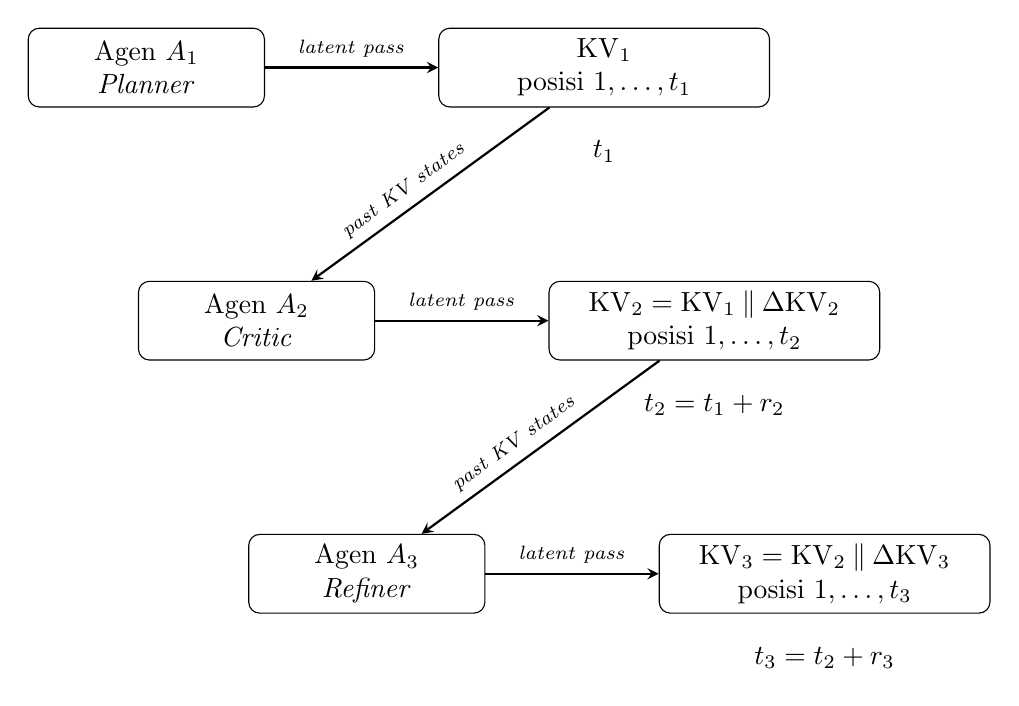
\begin{tikzpicture}[
        agent/.style={
            draw,
            rounded corners,
            align=center,
            minimum width=3.0cm,
            minimum height=10mm
        },
        cache/.style={
            draw,
            rounded corners,
            align=center,
            minimum width=4.2cm, % Sedikit dilebarkan agar teks KV2/KV3 muat
            minimum height=10mm
        },
        arrow/.style={
            ->,
            >=stealth,
            thick
        }
    ]

        % --- Baris 1 ---
        \node[agent] (a1) {Agen $A_1$\\\textit{Planner}};
        \node[cache, right=2.2cm of a1] (kv1) {$\mathrm{KV}_1$\\ posisi $1,\ldots,t_1$};
        
        % Panah latent pass: ke kanan
        \draw[arrow] (a1) -- node[above] {\scriptsize \textit{latent pass}} (kv1);

        % --- Baris 2 ---
        % A2 diletakkan di bawah kiri KV1
        \node[agent, below left=2.2cm and 0.8cm of kv1] (a2) {Agen $A_2$\\\textit{Critic}};
        
        % Panah past KV states: ke bawah kiri
        \draw[arrow] (kv1) -- node[above right, sloped, pos=0.85] {\scriptsize \textit{past KV states}} (a2);

        \node[cache, right=2.2cm of a2] (kv2) {$\mathrm{KV}_2 = \mathrm{KV}_1 \mathbin{\Vert} \Delta\mathrm{KV}_2$\\ posisi $1,\ldots,t_2$};
        
        % Panah latent pass: ke kanan
        \draw[arrow] (a2) -- node[above] {\scriptsize \textit{latent pass}} (kv2);

        % --- Baris 3 ---
        % A3 diletakkan di bawah kiri KV2
        \node[agent, below left=2.2cm and 0.8cm of kv2] (a3) {Agen $A_3$\\\textit{Refiner}};
        
        % Panah past KV states: ke bawah kiri
        \draw[arrow] (kv2) -- node[above right, sloped, pos=0.85] {\scriptsize \textit{past KV states}} (a3);

        \node[cache, right=2.2cm of a3] (kv3) {$\mathrm{KV}_3 = \mathrm{KV}_2 \mathbin{\Vert} \Delta\mathrm{KV}_3$\\ posisi $1,\ldots,t_3$};
        
        % Panah latent pass: ke kanan
        \draw[arrow] (a3) -- node[above] {\scriptsize \textit{latent pass}} (kv3);

        % --- Label Waktu ---
        \node[below=3mm of kv1] {$t_1$};
        \node[below=3mm of kv2] {$t_2=t_1+r_2$};
        \node[below=3mm of kv3] {$t_3=t_2+r_3$};

    \end{tikzpicture}

    \caption{Alur pewarisan dan pertumbuhan \textit{KV cache} antar-agen.}
    \label{fig:kv-agent-transfer}
\end{figure}

Pada komunikasi antar-agen, pertumbuhan tersebut terjadi tidak hanya ketika
satu agen memproses posisi baru, tetapi juga ketika \textit{KV cache} hasil
suatu agen diwariskan kepada agen berikutnya. Misalkan $t_i$ menyatakan jumlah
posisi yang telah tersimpan setelah agen ke-$i$ selesai diproses. Jika agen
ke-$(i+1)$ memproses sebanyak $r_{i+1}$ posisi baru, maka panjang cache
menjadi

\begin{equation}
    t_{i+1}
    =
    t_i+r_{i+1}.
    \label{eq:kv-agent-length}
\end{equation}

Dengan demikian, pada setiap lapisan,

\begin{equation}
    \mathrm{KV}^{(l)}_{i+1}
    =
    \mathrm{KV}^{(l)}_{i}
    \mathbin{\Vert}
    \Delta\mathrm{KV}^{(l)}_{i+1},
    \label{eq:kv-agent-growth}
\end{equation}

dengan $\Delta\mathrm{KV}^{(l)}_{i+1}$ menyatakan bagian \textit{KV cache}
yang terbentuk dari pemrosesan baru oleh agen ke-$(i+1)$.

Jika $r_i$ mencakup seluruh posisi baru yang diproses oleh agen ke-$i$,
termasuk posisi \textit{prompt} dan posisi yang berasal dari langkah laten,
maka panjang cache setelah $N$ agen dapat dituliskan sebagai

\begin{equation}
    t_N
    =
    \sum_{i=1}^{N} r_i.
    \label{eq:kv-total-length}
\end{equation}

Secara konseptual, pewarisan tersebut dapat diringkas sebagai

\begin{equation}
    \mathrm{KV}_1
    \longrightarrow
    \mathrm{KV}_2
    \longrightarrow
    \cdots
    \longrightarrow
    \mathrm{KV}_N,
    \label{eq:kv-agent-transfer}
\end{equation}

dengan setiap $\mathrm{KV}_i$ mempertahankan informasi yang telah tersimpan
sebelumnya dan menambahkan representasi dari posisi yang diproses oleh agen
ke-$i$.

%=============================================================

\section{Rancangan Eksperimen dan Analisis}
\label{sec:rancangan-eksperimen-analisis}


\subsection{Rancangan Eksperimen}
\label{subsec:rancangan-eksperimen}

Penelitian ini menggunakan eksperimen terkendali untuk membandingkan
formulasi representasi langkah laten dan medium komunikasi antar-agen
dalam \textit{Multi-Agent System} (MAS). Rancangan eksperimen dibentuk
dari dua aspek, yaitu medium komunikasi dan formulasi pembentukan representasi
langkah laten.

\begin{itemize}
    \item \textbf{Medium komunikasi:} berbasis teks dan berbasis
    \textit{KV-cache}.
    \item \textbf{Formulasi langkah laten (pada medium \textit{KV-cache}):}
    \texttt{raw}, \texttt{soft}, \texttt{sample}, dan \texttt{moi}.
\end{itemize}

Kondisi eksperimen terdiri atas satu kondisi komunikasi berbasis teks
dan empat kondisi berbasis \textit{KV-cache}:

\begin{itemize}
    \item Pada kondisi \texttt{text}, informasi antar-agen diteruskan
    sebagai keluaran tekstual sehingga tidak ada persamaan $\Phi$
    terpisah.
    \item Pada keempat kondisi lainnya, informasi diteruskan melalui
    \textit{KV-cache} dan representasi langkah laten dibentuk
    menggunakan persamaan $\Phi$ yang sesuai.
\end{itemize}

Struktur ini memungkinkan pengaruh medium komunikasi diuji dengan
membandingkan kondisi \texttt{text} terhadap kelompok kondisi
\textit{KV-cache}, sedangkan perbedaan antarformulasi laten dianalisis
dengan membandingkan keempat kondisi \textit{KV-cache}.

Secara ringkas, struktur perlakuan dapat dinyatakan sebagai

\begin{equation}
\mathcal{C}
=
\left\{
\texttt{text},
\texttt{raw},
\texttt{soft},
\texttt{sample},
\texttt{moi}
\right\},
\label{eq:kondisi-eksperimen}
\end{equation}

dengan

\begin{equation}
\begin{aligned}
\texttt{text}
&:\quad \text{medium teks},\\
\texttt{raw}
&:\quad \text{\textit{KV-cache} dengan }\Phi_{\texttt{raw}},\\
\texttt{soft}
&:\quad \text{\textit{KV-cache} dengan }\Phi_{\texttt{soft}},\\
\texttt{sample}
&:\quad \text{\textit{KV-cache} dengan }\Phi_{\texttt{sample}},\\
\texttt{moi}
&:\quad \text{\textit{KV-cache} dengan }\Phi_{\texttt{moi}}.
\end{aligned}
\label{eq:definisi-kondisi}
\end{equation}

Seluruh kondisi dijalankan menggunakan \textit{backbone} Qwen3-8B dan
rantai agen yang sama, yaitu
\textit{planner} $\rightarrow$ \textit{critic} $\rightarrow$
\textit{refiner} $\rightarrow$ \textit{judger}. Untuk kondisi yang
menggunakan langkah laten, setiap agen menjalankan paling banyak
$m=10$ langkah laten.

Faktor-faktor yang tidak menjadi objek perlakuan dijaga tetap sepanjang
eksperimen utama. Faktor tersebut mencakup model yang digunakan, struktur
rantai agen, jumlah maksimum langkah laten, parameter suhu pembentukan
distribusi langkah laten, parameter $\beta$ pada \textit{Mixture of
Inputs}, \textit{temperature} pembuatan keluaran teks, \textit{top-$p$}, batas panjang
keluaran, kriteria penghentian dini. Penetapan tersebut dilakukan agar
perbedaan hasil antarkondisi dapat dikaitkan dengan perlakuan yang
dibandingkan, bukan dengan perubahan konfigurasi eksperimen.

Evaluasi dilakukan pada GSM8K, ARC-Challenge, dan HumanEval+. Ketiga
\textit{benchmark} digunakan secara konsisten pada seluruh kondisi dalam
\textit{benchmark} yang sama. Pada setiap \textit{benchmark}, himpunan
soal yang digunakan juga dibuat identik untuk seluruh kondisi. Dengan
demikian, apabila kondisi $c_1,c_2\in\mathcal{C}$ dibandingkan pada soal
ke-$k$, hasil keduanya membentuk satu pasangan observasi,

\begin{equation}
\left(
Y_{k,c_1},
Y_{k,c_2}
\right),
\qquad
k=1,\ldots,n,
\label{eq:pasangan-observasi}
\end{equation}

dengan $Y_{k,c}$ menyatakan hasil evaluasi kondisi $c$ pada soal ke-$k$.
Struktur berpasangan tersebut digunakan karena setiap kondisi dievaluasi
pada objek soal yang sama, sehingga perbedaan tingkat kesulitan antar
himpunan soal tidak menjadi sumber perbedaan antarkondisi.

Secara keseluruhan, rancangan eksperimen dapat diringkas dalam alur
berikut.

\begin{figure}[H]
    \centering
    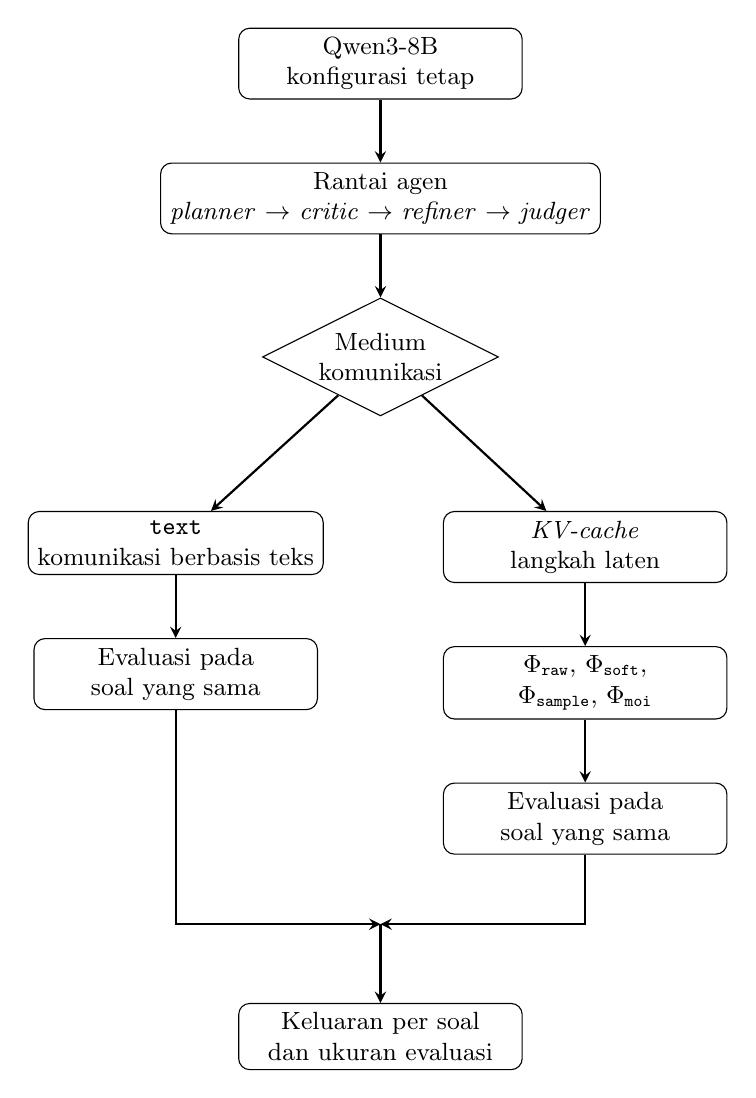
\begin{tikzpicture}[
        node distance=0.8cm,
        box/.style={
            rectangle,
            rounded corners,
            draw,
            align=center,
            minimum width=3.6cm,
            minimum height=0.8cm,
            font=\small
        },
        decision/.style={
            diamond,
            draw,
            align=center,
            aspect=2,
            inner sep=1pt,
            font=\small
        },
        arrow/.style={
            ->,
            >=stealth,
            thick
        }
    ]

        % --- Central spine ---
        \node[box] (model)
            {Qwen3-8B\\konfigurasi tetap};

        \node[box, below=of model] (mas)
            {Rantai agen\\\textit{planner} $\to$ \textit{critic}
             $\to$ \textit{refiner} $\to$ \textit{judger}};

        \node[decision, below=of mas] (medium)
            {Medium\\komunikasi};

        % --- Left branch: text ---
        \node[box, below=1.2cm of medium, xshift=-2.6cm] (text)
            {\texttt{text}\\komunikasi berbasis teks};

        \node[box, below=of text] (text_eval)
            {Evaluasi pada\\soal yang sama};

        % --- Right branch: KV-cache ---
        \node[box, below=1.2cm of medium, xshift=2.6cm] (kv)
            {\textit{KV-cache}\\langkah laten};

        \node[box, below=of kv] (formulation)
            {$\Phi_{\texttt{raw}}$, $\Phi_{\texttt{soft}}$,\\
             $\Phi_{\texttt{sample}}$, $\Phi_{\texttt{moi}}$};

        \node[box, below=of formulation] (kv_eval)
            {Evaluasi pada\\soal yang sama};

        % --- Merge point and result ---
        \path (text_eval.south) -- (kv_eval.south)
              coordinate[midway] (midAB);
        \coordinate (merge) at ([yshift=-1.8cm]midAB);

        \node[box, below=1.0cm of merge] (result)
            {Keluaran per soal\\dan ukuran evaluasi};

        % --- Arrows ---
        \draw[arrow] (model)       -- (mas);
        \draw[arrow] (mas)         -- (medium);
        \draw[arrow] (medium)      -- (text);
        \draw[arrow] (medium)      -- (kv);
        \draw[arrow] (text)        -- (text_eval);
        \draw[arrow] (kv)          -- (formulation);
        \draw[arrow] (formulation) -- (kv_eval);

        % --- Convergence to result ---
        \draw[arrow] (text_eval.south) |- (merge);
        \draw[arrow] (kv_eval.south)   |- (merge);
        \draw[arrow] (merge)           -- (result);

    \end{tikzpicture}
    \caption{Rancangan eksperimen penelitian.}
    \label{fig:rancangan-eksperimen}
\end{figure}

\subsection{Pengukuran dan Analisis Kinerja}
\label{subsec:pengukuran-analisis-kinerja}

Kinerja setiap kondisi eksperimen dievaluasi berdasarkan akurasi, \textit{format
rate}, jumlah token keluaran, dan waktu inferensi. Keempat ukuran dihitung pada
tingkat soal sehingga hasil dari soal yang sama pada kondisi berbeda dapat
dibandingkan secara berpasangan. Akurasi digunakan untuk mengukur proporsi
jawaban benar, sedangkan \textit{format rate} digunakan untuk mengukur proporsi
keluaran yang memenuhi format evaluasi. Definisi kedua ukuran tersebut mengacu
pada metrik yang telah dibahas pada Bab~\ref{sec:benchmark}.

Untuk kondisi $c$ pada suatu \textit{benchmark}, dengan $N$ soal, akurasi
dihitung sebagai

\begin{equation}
    A_c =
    \frac{1}{N}\sum_{i=1}^{N} I(Y_{ic}=1),
    \label{eq:akurasi-eksperimen}
\end{equation}

dengan $Y_{ic}=1$ apabila jawaban pada soal ke-$i$ dinyatakan benar dan
$Y_{ic}=0$ apabila dinyatakan salah. Sementara itu, \textit{format rate}
dihitung sebagai

\begin{equation}
    F_c =
    \frac{1}{N}\sum_{i=1}^{N} I(R_{ic}=1),
    \label{eq:format-rate-eksperimen}
\end{equation}

dengan $R_{ic}=1$ apabila keluaran dapat diproses oleh prosedur evaluasi dan
$R_{ic}=0$ sebaliknya.

Jumlah token keluaran dan waktu inferensi digunakan sebagai ukuran efisiensi.
Untuk masing-masing kondisi, nilai yang dilaporkan adalah rata-rata per soal,

\begin{equation}
    \bar{T}_c = \frac{1}{N}\sum_{i=1}^{N} T_{ic},
    \qquad
    \bar{W}_c = \frac{1}{N}\sum_{i=1}^{N} W_{ic},
    \label{eq:token-waktu}
\end{equation}

dengan $T_{ic}$ menyatakan jumlah token keluaran dan $W_{ic}$ menyatakan waktu
inferensi untuk soal ke-$i$ pada kondisi $c$.

\paragraph{Perbandingan berpasangan.}

Karena himpunan soal yang digunakan sama pada seluruh kondisi dalam satu
\textit{benchmark}, perbandingan dilakukan berdasarkan pasangan hasil pada
soal yang sama. Untuk dua kondisi $c_1$ dan $c_2$, pasangan pengamatan ke-$i$
dituliskan sebagai

\begin{equation}
    \left(Y_{ic_1},Y_{ic_2}\right),
    \qquad i=1,\ldots,N.
    \label{eq:pasangan-kinerja}
\end{equation}

Pendekatan berpasangan digunakan agar perbedaan tingkat kesulitan antarsoal
tidak diperlakukan sebagai variasi antarperlakuan.

\paragraph{Uji McNemar eksak.}

Perbedaan akurasi antara dua kondisi dianalisis menggunakan uji McNemar eksak.
Untuk setiap pasangan kondisi, banyaknya soal diklasifikasikan menjadi empat
kategori $a,b,c,d$, dengan $b$ dan $c$ menunjukkan hasil yang berbeda antara
kedua kondisi. Di bawah hipotesis nol

\begin{equation}
    H_0:\pi_b=\pi_c,
    \label{eq:h0-mcnemar-eksperimen}
\end{equation}

jumlah pasangan diskordan $b+c$ digunakan sebagai ukuran sampel pada distribusi
binomial dengan probabilitas $1/2$. Nilai-$p$ diperoleh secara eksak dari
distribusi tersebut. Pendekatan ini digunakan untuk menghindari ketergantungan
pada aproksimasi $\chi^2$ ketika jumlah pasangan diskordan relatif kecil.

\paragraph{\textit{Bootstrap} berpasangan.}

Untuk jumlah token dan waktu inferensi, ketidakpastian perbedaan antarkondisi
diukur menggunakan \textit{bootstrap} berpasangan. Untuk setiap soal
didefinisikan selisih

\begin{equation}
    D_i = X_{ic_1}-X_{ic_2},
    \qquad i=1,\ldots,N,
    \label{eq:selisih-bootstrap}
\end{equation}

dengan $X$ berupa jumlah token atau waktu inferensi. Indeks soal kemudian
di-\textit{resample} dengan pengembalian sehingga pasangan pengamatan tetap
dipertahankan. Statistik selisih dihitung pada setiap sampel ulang dan
interval kepercayaan $95\%$ diperoleh dari persentil ke-$2{,}5$ dan
ke-$97{,}5$ distribusi \textit{bootstrap}. Prosedur ini mengikuti konsep
\textit{bootstrap} yang telah dijelaskan pada Bab~\ref{sec:ujiberpasangan}.

\paragraph{Koreksi perbandingan berganda.}

Pengujian dilakukan untuk beberapa pasangan kondisi dan \textit{benchmark}.
Oleh karena itu, nilai-$p$ dari pengujian yang termasuk dalam satu kelompok
perbandingan disesuaikan menggunakan koreksi perbandingan berganda sebelum
interpretasi signifikansi dilakukan. Hasil analisis dilaporkan bersama
estimasi perbedaan dan interval kepercayaannya sehingga keputusan tidak hanya
didasarkan pada nilai-$p$.

\subsection{Benchmark dan Metrik Evaluasi}
\label{sec:benchmark}

Kemampuan model bahasa pada tugas bernalar diukur lewat tolok ukur
(\textit{benchmark}) baku: kumpulan soal beserta cara penilaian jawabannya
yang telah distandardisasi agar hasil dapat dibandingkan antarpenelitian.
Berikut tiga tolok ukur yang merentang jenis keluaran yang dituntut, dari
bilangan tunggal hingga kode program yang harus dieksekusi.

\textbf{GSM8K} \citep{gsm8k} berisi soal cerita matematika tingkat
sekolah dasar--menengah yang memerlukan beberapa langkah penalaran
aritmetika berurutan; jawaban akhir berupa satu bilangan.

\textbf{ARC-Challenge} \citep{arc} (\textit{AI2 Reasoning Challenge})
berisi soal sains pilihan ganda yang dipilih karena tidak terjawab benar
oleh pencocokan kata kunci sederhana, sehingga menuntut penalaran;
jawaban berupa satu simbol pilihan.

\textbf{HumanEval-Plus} \citep{humaneval,evalplus} berisi soal
pemrograman berupa tanda tangan fungsi beserta deskripsi tugasnya;
jawaban berupa kode program yang harus lolos serangkaian kasus uji unit.
Akhiran ``Plus'' menyatakan perluasan kasus uji oleh \citet{evalplus} yang
menutup celah himpunan uji asli \citep{humaneval}, sehingga solusi yang
tampak benar namun keliru pada kasus tepi lebih mungkin terdeteksi.

Ketiga tolok ukur di atas dinilai dengan metrik berikut.

\begin{definisi}
\label{def:akurasi}
Untuk $N$ soal dengan hasil benar/salah, \textit{akurasi} adalah proporsi
jawaban benar,
\begin{equation}
  \text{akurasi} = \frac{1}{N}\,
  \bigl|\{\,i : \text{jawaban ke-}i\text{ benar}\,\}\bigr|.
  \label{eq:akurasi}
\end{equation}
\end{definisi}

\begin{definisi}[\citealp{humaneval}]
\label{def:passk}
Untuk satu soal pemrograman, dibangkitkan $n\ge k$ sampel kode, dan
$c\le n$ di antaranya lolos seluruh kasus uji. \textit{Pass@k} adalah
peluang paling sedikit satu dari $k$ sampel yang dipilih acak (tanpa
pengembalian) dari $n$ sampel tersebut lolos, diestimasi tak bias lewat
\begin{equation}
  \text{pass@}k = \underset{\text{soal}}{\mathbb{E}}
  \left[\, 1 - \frac{\binom{n-c}{k}}{\binom{n}{k}} \,\right].
  \label{eq:passk}
\end{equation}
\end{definisi}

\begin{definisi}
\label{def:formatrate}
\textit{Format rate} adalah proporsi keluaran model yang mengikuti format
yang diminta (misalnya dapat diurai menjadi jawaban akhir atau kode yang
sintaksisnya sahih), terlepas dari benar-salahnya isi jawaban. Metrik ini
memisahkan kegagalan mengikuti format keluaran dari kegagalan substansi
jawaban.
\end{definisi}

\begin{definisi}
\label{def:biayakomputasi}
\textit{Biaya komputasi} suatu metode diukur lewat banyaknya token yang
diproses (masukan dan keluaran) dan/atau waktu inferensi (\textit{wall-clock
time}) per soal --- proksi baku untuk membandingkan efisiensi
antarmetode, karena tidak bergantung pada perangkat keras tertentu (peluang
token) atau langsung mencerminkan waktu tunggu pengguna (waktu inferensi).
\end{definisi}


\subsection{Pengukuran Geometris}
\label{subsec:pengukuran-geometris}

Pengukuran geometris digunakan untuk mengetahui posisi representasi langkah
laten yang dihasilkan oleh setiap formulasi relatif terhadap ruang representasi
token yang tersedia bagi model.

\subsubsection{Objek Representasi}

Keempat formulasi langkah laten menggunakan \textit{hidden state} yang sama
sebagai sumber informasi. Untuk suatu \textit{hidden state} $h$, persamaan
$\mathrm{mode}$ menghasilkan representasi laten

\begin{equation}
    z^{\mathrm{mode}}
    =
    \Phi_{\mathrm{mode}}(h),
    \qquad
    \mathrm{mode}
    \in
    \{
        \mathrm{raw},
        \mathrm{soft},
        \mathrm{sample},
        \mathrm{moi}
    \}.
    \label{eq:geo-objek-representasi}
\end{equation}

Dalam eksperimen, representasi tersebut telah dinormalisasi menggunakan norma
target $\tau$, sehingga

\begin{equation}
    z^{\mathrm{mode}}
    =
    \tau
    \frac{
        \widetilde{z}^{\mathrm{mode}}
    }{
        \left\|
            \widetilde{z}^{\mathrm{mode}}
        \right\|_2
    },
    \qquad
    \left\|
        z^{\mathrm{mode}}
    \right\|_2
    =
    \tau.
    \label{eq:geo-normalisasi}
\end{equation}

Normalisasi ini yang memungkinkan perbandingan antarmetode
difokuskan pada arah representasi. Dengan norma yang sama, perbedaan panjang
vektor tidak menjadi sumber perbedaan pada ukuran geometris yang digunakan.

\subsubsection{Ruang Pembanding}

Representasi laten dibandingkan dengan ruang \textit{input embedding} model.
Misalkan ukuran kosakata adalah $V$ dan dimensi representasi adalah $d$.
Matriks \textit{input embedding} dituliskan sebagai

\begin{equation}
    W_{\mathrm{in}}
    =
    \begin{bmatrix}
        W_{\mathrm{in}}[1]^{\mathsf T}\\
        W_{\mathrm{in}}[2]^{\mathsf T}\\
        \vdots\\
        W_{\mathrm{in}}[V]^{\mathsf T}
    \end{bmatrix}
    \in
    \mathbb{R}^{V\times d},
    \label{eq:geo-win}
\end{equation}

dengan

\begin{equation}
    W_{\mathrm{in}}[i]\in\mathbb{R}^{d}
\end{equation}

merupakan vektor \textit{embedding} untuk token ke-$i$.

Ruang pembanding tersebut dipilih karena $z^{\mathrm{mode}}$ digunakan kembali
sebagai representasi masukan pada langkah laten berikutnya. Dengan demikian,
pertanyaan geometris yang diuji adalah seberapa dekat representasi laten
tersebut dengan representasi token yang memang dapat diterima oleh model.

Hal ini berbeda dari membandingkan dengan $W_{\mathrm{out}}$. Matriks
$W_{\mathrm{out}}$ digunakan untuk memetakan \textit{hidden state} menjadi
\textit{logit}, sedangkan $W_{\mathrm{in}}$ merupakan ruang tempat vektor
representasi token diberikan kepada model. Karena $W_{\mathrm{in}}$ dan
$W_{\mathrm{out}}$ tidak diikat pada model yang digunakan, keduanya tidak
diasumsikan sebagai ruang geometris yang sama.

\subsubsection{Kemiripan Kosinus}

Kedekatan antara dua vektor diukur menggunakan kemiripan kosinus. Untuk dua
vektor tidak nol $u,v\in\mathbb{R}^{d}$, kemiripan kosinus didefinisikan sebagai

\begin{equation}
    \cos(u,v)
    =
    \frac{
        u^{\mathsf T}v
    }{
        \lVert u\rVert_2
        \lVert v\rVert_2
    }.
    \label{eq:geo-cosine}
\end{equation}

Persamaan~\eqref{eq:geo-cosine} membandingkan arah kedua vektor. Secara khusus, apabila

\begin{equation}
    u^{\mathsf T}v
    =
    \lVert u\rVert_2
    \lVert v\rVert_2,
\end{equation}

maka

\begin{equation}
    \cos(u,v)=1,
\end{equation}

yang menunjukkan bahwa kedua vektor memiliki arah yang sama. Sebaliknya,
nilai yang semakin kecil menunjukkan bahwa arah kedua vektor semakin berbeda.

\begin{figure}[htbp]
    \centering
    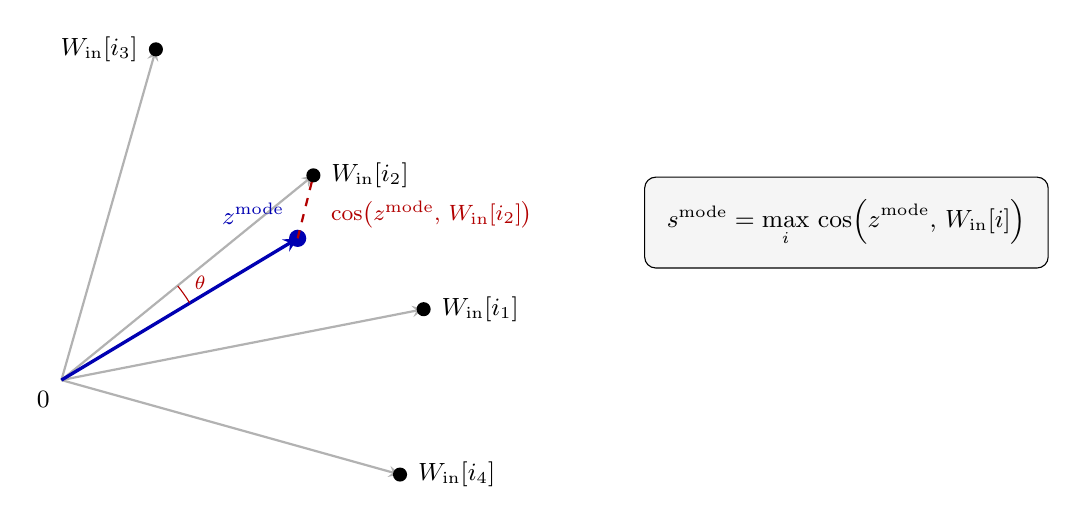
\begin{tikzpicture}[
        >=stealth,
        every node/.style={font=\small},
        vector/.style={->, thick, gray!60},
        zvec/.style={->, very thick, blue!70!black},
        token/.style={circle, fill=black, inner sep=1.8pt},
        latent/.style={circle, fill=blue!70!black, inner sep=2.2pt}
    ]

        \coordinate (O) at (0,0);

        % --- Token embedding vectors, disusun angular ---
        \coordinate (e1) at (4.6, 0.9);    %  ~11 derajat
        \coordinate (e2) at (3.2, 2.6);    %  ~39 derajat
        \coordinate (e3) at (1.2, 4.2);    %  ~74 derajat
        \coordinate (e4) at (4.3, -1.2);   % ~-16 derajat

        % --- Latent vector, arah paling dekat ke e2 ---
        \coordinate (z) at (3.0, 1.8);     %  ~31 derajat

        % --- Vektor ---
        \draw[vector] (O) -- (e1);
        \draw[vector] (O) -- (e2);
        \draw[vector] (O) -- (e3);
        \draw[vector] (O) -- (e4);
        \draw[zvec]   (O) -- (z);

        % --- Penanda titik ---
        \node[token]  at (e1) {};
        \node[token]  at (e2) {};
        \node[token]  at (e3) {};
        \node[token]  at (e4) {};
        \node[latent] at (z)  {};

        % --- Label embedding ---
        \node[right=3pt] at (e1) {$W_{\mathrm{in}}[i_1]$};
        \node[right=3pt] at (e2) {$W_{\mathrm{in}}[i_2]$};
        \node[left=3pt]  at (e3) {$W_{\mathrm{in}}[i_3]$};
        \node[right=3pt] at (e4) {$W_{\mathrm{in}}[i_4]$};

        % --- Label vektor laten ---
        \node[above left=2pt, blue!70!black] at (z) {$z^{\mathrm{mode}}$};

        % --- Garis putus-putus ke embedding paling mirip ---
        \draw[dashed, thick, red!70!black] (z) -- (e2);

        % --- Busur sudut theta ---
        \draw[red!70!black, thin]
            (31:1.9) arc[start angle=31, end angle=39, radius=1.9];
        \node[red!70!black, font=\scriptsize] at (35:2.15) {$\theta$};

        % --- Anotasi cosine, di kanan-tengah garis putus-putus ---
        \node[red!70!black, font=\footnotesize, anchor=west]
            at ($(z)!0.5!(e2) + (0.20, -0.10)$)
            {$\cos\!\left(z^{\mathrm{mode}},\, W_{\mathrm{in}}[i_2]\right)$};

        % --- Origin ---
        \node[below left=1pt] at (O) {$0$};

        % --- Panel rumus, dipisah dari diagram ---
        \node[
            draw, rounded corners, fill=gray!8,
            inner sep=8pt, align=center, anchor=west
        ] at (7.4, 2.0)
            {$s^{\mathrm{mode}} =
              \displaystyle\max_{i}\,
              \cos\!\left(z^{\mathrm{mode}},\, W_{\mathrm{in}}[i]\right)$};

    \end{tikzpicture}
    \caption{%
        Ilustrasi konseptual pengukuran geometris. Vektor $z^{\mathrm{mode}}$
        dibandingkan dengan seluruh vektor \textit{input embedding}
        $W_{\mathrm{in}}[i]$, kemudian kemiripan kosinus terbesar digunakan
        sebagai ukuran kedekatan geometris.}
    \label{fig:pengukuran-geometris}
\end{figure}

Untuk sebuah representasi laten $z^{\mathrm{mode}}$, kemiripan terhadap seluruh
kosakata dihitung dengan

\begin{equation}
    s_i^{\mathrm{mode}}
    =
    \cos
    \left(
        z^{\mathrm{mode}},
        W_{\mathrm{in}}[i]
    \right),
    \qquad
    i=1,\ldots,V.
    \label{eq:geo-cosine-token}
\end{equation}

Karena tujuan pengukuran adalah mengetahui apakah terdapat setidaknya satu
\textit{embedding} token yang memiliki arah dekat dengan representasi laten,
nilai maksimum digunakan sebagai ukuran kedekatan geometris,

\begin{equation}
    s^{\mathrm{mode}}
    =
    \max_{1\leq i\leq V}
    \cos
    \left(
        z^{\mathrm{mode}},
        W_{\mathrm{in}}[i]
    \right).
    \label{eq:geo-max-cosine}
\end{equation}

Persamaan~\eqref{eq:geo-max-cosine} tidak menyatakan bahwa token dengan
kemiripan maksimum tersebut merupakan token yang benar atau token yang
kemudian dihasilkan model. Ukuran tersebut hanya menyatakan apakah terdapat
arah pada ruang \textit{embedding} token yang dekat dengan representasi laten.

Nilai $s^{\mathrm{mode}}$ yang semakin mendekati $1$ menunjukkan bahwa
representasi laten semakin dekat secara arah dengan setidaknya satu
\textit{embedding} token. Sebaliknya, nilai yang lebih rendah menunjukkan
bahwa representasi tersebut lebih jauh dari seluruh arah \textit{embedding}
token.



\subsubsection{Agregasi Pengukuran}

Satu soal menghasilkan beberapa representasi laten karena setiap agen dapat
menjalankan beberapa langkah laten. Oleh karena itu, nilai
$s^{\mathrm{mode}}$ pada Persamaan~\eqref{eq:geo-max-cosine} terlebih dahulu
dihitung pada setiap langkah laten.

Misalkan $q$ menyatakan indeks soal, $a$ indeks agen, dan $k$ indeks langkah
laten. Kedekatan geometris pada satu posisi representasi didefinisikan sebagai

\begin{equation}
    s_{qak}^{\mathrm{mode}}
    =
    \max_{1\leq i\leq V}
    \cos
    \left(
        z_{qak}^{\mathrm{mode}},
        W_{\mathrm{in}}[i]
    \right).
    \label{eq:geo-score-position}
\end{equation}

Untuk memperoleh satu ukuran geometris pada tingkat agen dan soal, nilai
tersebut dirata-ratakan sepanjang langkah laten yang benar-benar dihasilkan.
Jika $K_{qa}^{\mathrm{mode}}$ adalah jumlah langkah laten pada agen $a$ untuk
soal $q$, maka

\begin{equation}
    \bar{s}_{qa}^{\mathrm{mode}}
    =
    \frac{1}{K_{qa}^{\mathrm{mode}}}
    \sum_{k=1}^{K_{qa}^{\mathrm{mode}}}
    s_{qak}^{\mathrm{mode}}.
    \label{eq:geo-agregasi-langkah}
\end{equation}

Agregasi selanjutnya dilakukan pada tingkat agen. Dengan $A$ menyatakan
jumlah agen dalam rantai,

\begin{equation}
    \bar{s}_{q}^{\mathrm{mode}}
    =
    \frac{1}{A}
    \sum_{a=1}^{A}
    \bar{s}_{qa}^{\mathrm{mode}}.
    \label{eq:geo-agregasi-agen}
\end{equation}

Nilai $\bar{s}_{q}^{\mathrm{mode}}$ kemudian menjadi ukuran geometris pada
tingkat soal. Untuk $N$ soal, ukuran agregat suatu persamaan dihitung sebagai

\begin{equation}
    \overline{s}^{\mathrm{mode}}
    =
    \frac{1}{N}
    \sum_{q=1}^{N}
    \bar{s}_{q}^{\mathrm{mode}}.
    \label{eq:geo-agregasi-soal}
\end{equation}

Dengan struktur tersebut, agregasi dilakukan secara bertahap,

\begin{equation}
    s_{qak}^{\mathrm{mode}}
    \longrightarrow
    \bar{s}_{qa}^{\mathrm{mode}}
    \longrightarrow
    \bar{s}_{q}^{\mathrm{mode}}
    \longrightarrow
    \overline{s}^{\mathrm{mode}}.
    \label{eq:geo-hierarchical-aggregation}
\end{equation}

Urutan tersebut mempertahankan unit soal sebagai unit observasi pada analisis
selanjutnya. Hal ini memungkinkan ukuran geometris dibandingkan dengan hasil
keluaran pada soal yang sama.

\subsubsection{Hubungan dengan Keluaran}

Ukuran geometris digunakan sebagai variabel representasi, sedangkan keluaran
tugas digunakan sebagai ukuran kinerja. Untuk soal ke-$q$, keberhasilan
keluaran dituliskan sebagai variabel indikator

\begin{equation}
    Y_q^{\mathrm{mode}}
    =
    \mathbb{1}
    \left[
        \text{keluaran ke-$q$ benar}
    \right].
    \label{eq:geo-output-indicator}
\end{equation}

Dengan demikian, setiap soal memiliki pasangan

\begin{equation}
    \left(
        \bar{s}_{q}^{\mathrm{mode}},
        Y_q^{\mathrm{mode}}
    \right),
    \qquad
    q=1,\ldots,N.
    \label{eq:geo-output-pair}
\end{equation}

Pasangan tersebut digunakan untuk melihat apakah perubahan karakteristik
geometris muncul bersamaan dengan perubahan pada keluaran. Pada tingkat
agregat, akurasi tetap dihitung dari

\begin{equation}
    A^{\mathrm{mode}}
    =
    \frac{1}{N}
    \sum_{q=1}^{N}
    Y_q^{\mathrm{mode}},
    \label{eq:geo-accuracy}
\end{equation}

sedangkan karakteristik geometris diringkas melalui

\begin{equation}
    \overline{s}^{\mathrm{mode}}
    =
    \frac{1}{N}
    \sum_{q=1}^{N}
    \bar{s}_{q}^{\mathrm{mode}}.
    \label{eq:geo-final-summary}
\end{equation}

Perbandingan $A^{\mathrm{mode}}$ dan $\overline{s}^{\mathrm{mode}}$ digunakan
sebagai analisis deskriptif untuk melihat apakah formulasi dengan karakteristik
geometris yang berbeda juga menunjukkan pola kinerja yang berbeda. Hubungan
tersebut tidak dimaksudkan sebagai hubungan sebab-akibat. Kedekatan geometris
hanya memberikan bukti mengenai karakteristik representasi yang dapat
digunakan untuk membantu menjelaskan perbedaan keluaran.

\subsection{Interpolasi Geometris}
\label{subsec:interpolasi-geometris}

Pengukuran geometris pada Subbab~\ref{subsec:pengukuran-geometris}
memberikan ukuran kedekatan masing-masing representasi laten terhadap ruang
\textit{embedding} masukan. Namun, perbandingan antara dua persamaan hanya
memberikan informasi pada dua titik representasi. Untuk mengamati perubahan
kinerja sepanjang perpindahan dari formulasi \textit{raw} menuju formulasi
\textit{soft}, digunakan interpolasi geometris.

Interpolasi dilakukan pada keluaran akhir kedua formulasi, yaitu
$\Phi_{\texttt{raw}}(h)$ dan $\Phi_{\texttt{soft}}(h)$. Kedua vektor tersebut
telah dinormalisasi menggunakan norma yang sama $\tau$ sebagaimana pada
Pers.~\eqref{eq:geo-normalisasi}. Untuk $\alpha\in[0,1]$, mula-mula dibentuk
vektor campuran

\begin{equation}
u_{\alpha}
=
(1-\alpha)\Phi_{\texttt{raw}}(h)
+
\alpha\Phi_{\texttt{soft}}(h).
\label{eq:m-interp-u}
\end{equation}

Vektor campuran tersebut kemudian dinormalisasi kembali ke norma $\tau$,

\begin{equation}
\boxed{
\Phi_{\mathrm{mix}}^{(\alpha)}(h)
=
\tau
\frac{u_{\alpha}}
{\lVert u_{\alpha}\rVert}
}
\qquad
u_{\alpha}\neq\mathbf{0}.
\label{eq:m-interp}
\end{equation}

Pers.~\eqref{eq:m-interp-u} menentukan arah pencampuran antara kedua
representasi, sedangkan Pers.~\eqref{eq:m-interp} memastikan bahwa representasi
yang digunakan pada setiap nilai $\alpha$ memiliki magnitudo yang sama.
Dengan demikian,

\begin{equation}
\left\lVert
\Phi_{\mathrm{mix}}^{(\alpha)}(h)
\right\rVert
=
\tau,
\qquad
\forall\alpha\in[0,1].
\label{eq:m-interp-norm}
\end{equation}

Pilihan ini membuat perubahan representasi sepanjang interpolasi dapat
dipandang terutama sebagai perubahan arah pada ruang laten.

\paragraph{Titik ujung interpolasi.}

Konstruksi pada Pers.~\eqref{eq:m-interp} mempertahankan kedua formulasi asal
secara tepat pada titik ujung $\alpha=0$ dan $\alpha=1$. Untuk $\alpha=0$,
diperoleh

\begin{align}
u_0
&=
(1-0)\Phi_{\texttt{raw}}(h)
+
0\Phi_{\texttt{soft}}(h)
\nonumber\\
&=
\Phi_{\texttt{raw}}(h).
\end{align}

Karena $\lVert\Phi_{\texttt{raw}}(h)\rVert=\tau$, maka

\begin{align}
\Phi_{\mathrm{mix}}^{(0)}(h)
&=
\tau
\frac{\Phi_{\texttt{raw}}(h)}
{\lVert\Phi_{\texttt{raw}}(h)\rVert}
\nonumber\\
&=
\tau
\frac{\Phi_{\texttt{raw}}(h)}
{\tau}
\nonumber\\
&=
\Phi_{\texttt{raw}}(h).
\label{eq:m-interp-end-raw}
\end{align}

Dengan cara yang sama, untuk $\alpha=1$,

\begin{align}
u_1
&=
\Phi_{\texttt{soft}}(h),
\\
\Phi_{\mathrm{mix}}^{(1)}(h)
&=
\tau
\frac{\Phi_{\texttt{soft}}(h)}
{\lVert\Phi_{\texttt{soft}}(h)\rVert}
\nonumber\\
&=
\Phi_{\texttt{soft}}(h).
\label{eq:m-interp-end-soft}
\end{align}

Dengan demikian,

\begin{equation}
\boxed{
\Phi_{\mathrm{mix}}^{(0)}(h)
=
\Phi_{\texttt{raw}}(h),
\qquad
\Phi_{\mathrm{mix}}^{(1)}(h)
=
\Phi_{\texttt{soft}}(h)
}.
\label{eq:m-interp-endpoints}
\end{equation}

Pers.~\eqref{eq:m-interp-endpoints} menunjukkan bahwa interpolasi tidak
menghasilkan perubahan pada kedua kondisi pembatas. Kondisi $\alpha=0$
identik dengan formulasi \textit{raw}, sedangkan $\alpha=1$ identik dengan
formulasi \textit{soft}. Oleh karena itu, kedua titik ujung dapat menggunakan
hasil eksperimen yang telah diperoleh sebelumnya.

\paragraph{Lintasan geometris.}

Selanjutnya, misalkan

\begin{equation}
a=\Phi_{\texttt{raw}}(h),
\qquad
b=\Phi_{\texttt{soft}}(h),
\qquad
\lVert a\rVert=\lVert b\rVert=\tau.
\label{eq:m-interp-ab}
\end{equation}

Sebelum normalisasi, $u_\alpha$ merupakan kombinasi linear dari $a$ dan $b$.
Oleh karena itu,

\begin{equation}
u_\alpha
=
(1-\alpha)a+\alpha b
\in
\operatorname{span}\{a,b\}.
\label{eq:m-interp-span}
\end{equation}

Ketika $u_\alpha$ dinormalisasi ke norma $\tau$, setiap titik pada ruas garis
yang menghubungkan $a$ dan $b$ diproyeksikan kembali ke bola berjari-jari
$\tau$. Karena seluruh ruas tersebut berada pada bidang yang dibentuk oleh
$a$ dan $b$, lintasan hasil normalisasi berada pada irisan bidang tersebut
dengan bola, yaitu suatu lingkaran besar (\textit{great circle}).

Dengan demikian, untuk $u_\alpha\neq\mathbf{0}$,

\begin{equation}
\Phi_{\mathrm{mix}}^{(\alpha)}(h)
\in
\left\{
z\in\mathbb{R}^{d}
:
\lVert z\rVert=\tau
\right\},
\label{eq:m-interp-sphere}
\end{equation}

dan lintasan $\alpha\mapsto\Phi_{\mathrm{mix}}^{(\alpha)}(h)$ bergerak dari
$\Phi_{\texttt{raw}}(h)$ menuju $\Phi_{\texttt{soft}}(h)$ pada bola tersebut.

Kasus $u_\alpha=\mathbf{0}$ hanya dapat terjadi ketika kedua vektor berlawanan
arah. Karena $\lVert a\rVert=\lVert b\rVert=\tau$, kondisi tersebut mensyaratkan

\begin{equation}
b=-a,
\qquad
\alpha=\frac12,
\label{eq:m-interp-zero}
\end{equation}

yang ekuivalen dengan

\begin{equation}
\cos(a,b)=-1.
\end{equation}

Pada kondisi tersebut normalisasi pada Pers.~\eqref{eq:m-interp} tidak
terdefinisi. Oleh karena itu, interpolasi hanya didefinisikan untuk nilai
$\alpha$ yang menghasilkan $u_\alpha\neq\mathbf{0}$.

\paragraph{Hubungan $\alpha$ dengan perpindahan sudut.}

Parameter $\alpha$ menentukan bobot pencampuran, tetapi tidak secara langsung
menentukan jarak geometris pada bola. Untuk melihat hubungan tersebut,
misalkan $\theta$ adalah sudut antara $a$ dan $b$,

\begin{equation}
\theta
=
\arccos
\left(
\frac{a^\top b}
{\lVert a\rVert\lVert b\rVert}
\right).
\label{eq:m-interp-theta}
\end{equation}

Definisikan vektor satuan

\begin{equation}
\hat a=\frac{a}{\tau},
\end{equation}

serta $\hat n$ sebagai vektor satuan yang berada pada
$\operatorname{span}\{a,b\}$ dan tegak lurus terhadap $\hat a$. Dengan
demikian, $b$ dapat dituliskan sebagai

\begin{equation}
b
=
\tau
\left(
\cos\theta\,\hat a
+
\sin\theta\,\hat n
\right).
\label{eq:m-interp-basis}
\end{equation}

Substitusi Pers.~\eqref{eq:m-interp-basis} ke Pers.~\eqref{eq:m-interp-u}
menghasilkan

\begin{align}
u_\alpha
&=
(1-\alpha)\tau\hat a
+
\alpha\tau
\left(
\cos\theta\,\hat a
+
\sin\theta\,\hat n
\right)
\nonumber\\
&=
\tau
\left[
\left(
(1-\alpha)+\alpha\cos\theta
\right)\hat a
+
\alpha\sin\theta\,\hat n
\right].
\label{eq:m-interp-decomp}
\end{align}

Jika $\varphi(\alpha)$ menyatakan sudut antara $a$ dan
$\Phi_{\mathrm{mix}}^{(\alpha)}(h)$, maka dari komponen yang sejajar dan
tegak lurus terhadap $\hat a$ diperoleh

\begin{equation}
\boxed{
\tan\varphi(\alpha)
=
\frac{
\alpha\sin\theta
}{
(1-\alpha)+\alpha\cos\theta
}
}.
\label{eq:m-interp-angle}
\end{equation}

Pers.~\eqref{eq:m-interp-angle} menunjukkan bahwa perubahan $\alpha$ tidak
secara umum menghasilkan perubahan sudut yang linear. Sebagai contoh, pada
$\alpha=\frac12$,

\begin{align}
\tan\varphi\left(\frac12\right)
&=
\frac{\frac12\sin\theta}
{\frac12+\frac12\cos\theta}
\nonumber\\
&=
\frac{\sin\theta}{1+\cos\theta}
\nonumber\\
&=
\tan\frac{\theta}{2}.
\end{align}

Sehingga

\begin{equation}
\varphi\left(\frac12\right)
=
\frac{\theta}{2}.
\label{eq:m-interp-midpoint}
\end{equation}

Hasil tersebut menunjukkan bahwa titik tengah pencampuran setelah
normalisasi berada pada titik tengah busur antara kedua representasi.
Namun, di luar titik tengah tersebut, jarak sudut tidak berubah secara
linear terhadap $\alpha$. Oleh karena itu, $\alpha$ diperlakukan sebagai
parameter pencampuran, bukan sebagai ukuran jarak geometris.

\paragraph{Kisi interpolasi.}

Eksperimen interpolasi menggunakan kisi

\begin{equation}
\boxed{
\alpha
\in
\{0,\;0{,}25,\;0{,}50,\;0{,}75,\;1\}.
}
\label{eq:m-alpha-grid}
\end{equation}

Nilai $\alpha=0$ dan $\alpha=1$ masing-masing merepresentasikan formulasi
\textit{raw} dan \textit{soft} berdasarkan Pers.~\eqref{eq:m-interp-endpoints}.
Dengan demikian, hanya tiga nilai tengah yang memerlukan kondisi eksperimen
tambahan.

Kisi tersebut memberikan tiga titik di antara kedua formulasi, yaitu
$\alpha=0{,}25$, $\alpha=0{,}50$, dan $\alpha=0{,}75$. Ketiga titik tersebut
digunakan untuk mengamati bentuk perubahan kinerja sepanjang lintasan,
bukan hanya perbedaan pada kedua titik ujung.

Interpolasi dijalankan pada HumanEval+ dengan menggunakan pertanyaan yang
sama seperti eksperimen utama. Pemilihan ini mengikuti rancangan eksperimen
yang menggunakan interpolasi sebagai analisis tambahan pada kondisi dengan
perbedaan kinerja antara \textit{raw} dan formulasi berbasis token yang lebih
jelas.

\paragraph{Pengukuran posisi geometris sepanjang interpolasi.}

Karena $\alpha$ merupakan bobot pencampuran dan bukan ukuran jarak geometris,
posisi representasi sepanjang lintasan diukur kembali menggunakan ukuran
geometris pada Subbab~\ref{subsec:pengukuran-geometris}. Untuk setiap
$\alpha$, didefinisikan

\begin{equation}
s(\alpha)
=
\max_{1\leq i\leq V}
\cos
\left(
\Phi_{\mathrm{mix}}^{(\alpha)}(h),
W_{\mathrm{in}}[i]
\right).
\label{eq:m-interp-score}
\end{equation}

Dengan demikian, terdapat dua besaran yang berbeda. Parameter $\alpha$
menentukan bagaimana representasi \textit{raw} dan \textit{soft} dicampurkan,
sedangkan $s(\alpha)$ mengukur posisi representasi hasil pencampuran relatif
terhadap ruang \textit{embedding} token.

Hubungan keduanya kemudian dapat digunakan untuk membandingkan perubahan
keluaran model dengan perubahan posisi geometris. Secara khusus, untuk setiap
nilai $\alpha$ dicatat keluaran model dan ukuran geometris
$s(\alpha)$, sehingga pasangan pengamatan dapat dituliskan sebagai

\begin{equation}
\left(
s(\alpha),Y^{(\alpha)}
\right),
\label{eq:m-interp-observation}
\end{equation}

dengan $Y^{(\alpha)}$ menyatakan indikator keberhasilan keluaran pada nilai
$\alpha$ tersebut. Analisis ini digunakan untuk mengamati apakah perubahan kinerja berjalan
searah dengan perubahan kedekatan representasi terhadap ruang
\textit{embedding} token.



% ---------------------------------------------------------------------------
% Daftar Pustaka
% ---------------------------------------------------------------------------
% ============================================================================
% DAFTAR PUSTAKA — manual (natbib), urut abjad menurut nama penulis pertama.
% Syarat bimbingan: WAJIB \href ke sumber unduhan; jangan menyitir skripsi S1.
% Penulis paper inti (QuantaAlpha, LatentMAS) sudah dilengkapi dari arXiv.
% Catatan: daftar penulis QuantaAlpha memakai "dkk." (kolaborasi besar);
% cocokkan daftar penuh dengan versi terbit final sebelum sidang.
% ============================================================================
\begin{thebibliography}{99}
\addcontentsline{toc}{chapter}{DAFTAR PUSTAKA}

\bibitem[Agresti(2013)]{agresti}
Agresti, A. (2013).
\href{https://archive.org/details/categoricaldataa0000agre}{\emph{Categorical
Data Analysis}} (3rd ed.). Hoboken: John Wiley \& Sons.

\bibitem[Ainslie dkk(2023)]{ainslie}
Ainslie, J., Lee-Thorp, J., de Jong, M., Zemlyanskiy, Y., Lebr\'{o}n, F., \&
Sanghai, S. (2023).
\href{https://arxiv.org/abs/2305.13245}{GQA: Training generalized multi-query
transformer models from multi-head checkpoints}. \emph{Proceedings of the 2023
Conference on Empirical Methods in Natural Language Processing (EMNLP)},
4895--4901.

\bibitem[Anthropic(2025)]{anthropicpricing}
Anthropic. (2025).
\href{https://docs.claude.com/en/docs/about-claude/pricing}{Pricing}.
\emph{Claude Platform Documentation}. Diakses pada 3 September 2026.

\bibitem[Anton dan Rorres(2010)]{anton}
Anton, H., \& Rorres, C. (2010).
\href{https://archive.org/details/elementarylinea000anto}{\emph{Elementary
Linear Algebra: Applications Version}} (10th ed.). Hoboken: John Wiley \& Sons.

\bibitem[Austin dkk(2021)]{mbpp}
Austin, J., Odena, A., Nye, M., Bosma, M., Michalewski, H., Dohan, D.,
Jiang, E., Cai, C., Terry, M., Le, Q., \& Sutton, C. (2021).
\href{https://arxiv.org/abs/2108.07732}{Program synthesis with large language
models}. \emph{arXiv preprint} arXiv:2108.07732.

\bibitem[Bain dan Engelhardt(1992)]{bain}
Bain, L. J., \& Engelhardt, M. (1992).
\href{https://archive.org/details/introductiontopr0000bain}{\emph{Introduction
to Probability and Mathematical Statistics}} (2nd ed.). Boston: PWS-KENT.

\bibitem[Bishop(2006)]{bishop}
Bishop, C. M. (2006).
\href{https://www.microsoft.com/en-us/research/uploads/prod/2006/01/Bishop-Pattern-Recognition-and-Machine-Learning-2006.pdf}{\emph{Pattern
Recognition and Machine Learning}}. New York: Springer.

\bibitem[Boyd dan Vandenberghe(2004)]{boyd}
Boyd, S., \& Vandenberghe, L. (2004).
\href{https://web.stanford.edu/~boyd/cvxbook/bv_cvxbook.pdf}{\emph{Convex
Optimization}}. Cambridge: Cambridge University Press.

\bibitem[Casella dan Berger(2002)]{casella}
Casella, G., \& Berger, R. L. (2002).
\href{https://archive.org/details/statisticalinfer0000case}{\emph{Statistical
Inference}} (2nd ed.). Pacific Grove: Duxbury.

\bibitem[Chen dkk(2021)]{humaneval}
Chen, M., Tworek, J., Jun, H., Yuan, Q., Pinto, H. P. de O., Kaplan, J., dkk.
(2021). \href{https://arxiv.org/abs/2107.03374}{Evaluating large language
models trained on code}. \emph{arXiv preprint} arXiv:2107.03374.

\bibitem[Chen dkk(2025)]{latentsurvey}
Chen, X., dkk. (2025).
\href{https://arxiv.org/abs/2505.16782}{\emph{Reasoning beyond language: A
comprehensive survey on latent chain-of-thought reasoning}}. arXiv:2505.16782.

\bibitem[Clark dkk(2018)]{arc}
Clark, P., Cowhey, I., Etzioni, O., Khot, T., Sabharwal, A., Schoenick, C., \&
Tafjord, O. (2018). \href{https://arxiv.org/abs/1803.05457}{Think you have
solved question answering? Try ARC, the AI2 Reasoning Challenge}.
\emph{arXiv preprint} arXiv:1803.05457.

\bibitem[Cobbe dkk(2021)]{gsm8k}
Cobbe, K., Kosaraju, V., Bavarian, M., Chen, M., Jun, H., Kaiser, L., dkk.
(2021). \href{https://arxiv.org/abs/2110.14168}{Training verifiers to solve
math word problems}. \emph{arXiv preprint} arXiv:2110.14168.

\bibitem[Cover dan Thomas(2006)]{cover}
Cover, T. M., \& Thomas, J. A. (2006).
\href{https://github.com/Bladefidz/information-theory/blob/master/books/Elements%20of%20Information%20Theory.pdf}{\emph{Elements
of Information Theory}} (2nd ed.). Hoboken: John Wiley \& Sons.

\bibitem[Efron dan Tibshirani(1993)]{efron}
Efron, B., \& Tibshirani, R. J. (1993).
\href{https://archive.org/details/introductiontobo0000efro}{\emph{An Introduction
to the Bootstrap}}. New York: Chapman \& Hall.

\bibitem[Fama dan French(2015)]{famafrench}
Fama, E. F., \& French, K. R. (2015).
\href{https://doi.org/10.1016/j.jfineco.2014.10.010}{A five-factor asset pricing
model}. \emph{Journal of Financial Economics}, 116(1), 1--22.

\bibitem[Finin dkk(1994)]{kqml}
Finin, T., Fritzson, R., McKay, D., \& McEntire, R. (1994).
\href{https://doi.org/10.1145/191246.191322}{KQML as an agent communication
language}. \emph{Proceedings of the 3rd International Conference on Information
and Knowledge Management (CIKM)}, 456--463.

\bibitem[Friedman(2001)]{friedman}
Friedman, J. H. (2001).
\href{https://doi.org/10.1214/aos/1013203451}{Greedy function approximation:
A gradient boosting machine}. \emph{The Annals of Statistics}, 29(5),
1189--1232.

\bibitem[Fu dkk(2025)]{cache2cache}
Fu, T., dkk. (2025).
\href{https://arxiv.org/abs/2510.03215}{\emph{Cache-to-Cache: Direct semantic
communication between large language models}}. arXiv:2510.03215.

\bibitem[Gelman dkk(2013)]{gelman}
Gelman, A., Carlin, J. B., Stern, H. S., Dunson, D. B., Vehtari, A., \&
Rubin, D. B. (2013).
\href{https://sites.stat.columbia.edu/gelman/book/BDA3.pdf}{\emph{Bayesian
Data Analysis}} (3rd ed.). Boca Raton: CRC Press.

\bibitem[Golub dan Van Loan(2013)]{golub}
Golub, G. H., \& Van Loan, C. F. (2013).
\href{https://archive.org/details/matrixcomputatio0004golu}{\emph{Matrix
Computations}} (4th ed.). Baltimore: Johns Hopkins University Press.

\bibitem[Goodfellow dkk(2016)]{goodfellow}
Goodfellow, I., Bengio, Y., \& Courville, A. (2016).
\href{https://www.deeplearningbook.org}{\emph{Deep Learning}}.
Cambridge: MIT Press.

\bibitem[Grinold dan Kahn(2000)]{grinold}
Grinold, R. C., \& Kahn, R. N. (2000).
\href{https://archive.org/details/activeportfoliom0000grin}{\emph{Active
Portfolio Management: A Quantitative Approach for Producing Superior Returns
and Controlling Risk}} (2nd ed.). New York: McGraw-Hill.

\bibitem[Gumbel(1958)]{gumbel}
Gumbel, E. J. (1958).
\href{https://archive.org/details/statisticsofextr0000gumb}{\emph{Statistics of
Extremes}}. New York: Columbia University Press.

\bibitem[Guo dkk(2024)]{guo}
Guo, T., Chen, X., Wang, Y., Chang, R., Pei, S., Chawla, N. V., Wiest, O., \&
Zhang, X. (2024).
\href{https://arxiv.org/abs/2402.01680}{\emph{Large language model based
multi-agents: A survey of progress and challenges}}. arXiv:2402.01680.

\bibitem[Han dkk(2026)]{quantaalpha}
Han, J., Zhang, S., Li, W., Dong, Y., Hu, T., dkk. (2026).
\href{https://arxiv.org/abs/2602.07085}{\emph{QuantaAlpha: An Evolutionary
Framework for LLM-Driven Alpha Mining}}. arXiv:2602.07085.

\bibitem[Hao dkk(2024)]{coconut}
Hao, S., Sukhbaatar, S., Su, D., Li, X., Hu, Z., Weston, J., \& Tian, Y. (2024).
\href{https://arxiv.org/abs/2412.06769}{\emph{Training large language models to
reason in a continuous latent space}}. arXiv:2412.06769.

\bibitem[Hastie dkk(2009)]{hastie}
Hastie, T., Tibshirani, R., \& Friedman, J. (2009).
\href{https://archive.org/details/elementsofstatis0000hast}{\emph{The
Elements of Statistical Learning: Data Mining, Inference, and Prediction}}
(2nd ed.). New York: Springer.

\bibitem[Hoerl dan Kennard(1970)]{ridge}
Hoerl, A. E., \& Kennard, R. W. (1970).
\href{https://doi.org/10.1080/00401706.1970.10488634}{Ridge regression: Biased
estimation for nonorthogonal problems}. \emph{Technometrics}, 12(1), 55--67.

\bibitem[Holtzman dkk(2020)]{holtzman}
Holtzman, A., Buys, J., Du, L., Forbes, M., \& Choi, Y. (2020).
\href{https://arxiv.org/abs/1904.09751}{The curious case of neural text
degeneration}. \emph{International Conference on Learning Representations
(ICLR)}.

\bibitem[IBM(2025)]{ibmbreach}
IBM. (2025).
\href{https://www.ibm.com/think/x-force/2025-cost-of-a-data-breach-navigating-ai}{2025
Cost of a Data Breach Report: Navigating the AI rush without sidelining
security}. Armonk: IBM Corporation. Diakses pada 3 September 2026.

\bibitem[Jang dkk(2017)]{jang}
Jang, E., Gu, S., \& Poole, B. (2017).
\href{https://arxiv.org/abs/1611.01144}{Categorical reparameterization with
Gumbel-Softmax}. \emph{International Conference on Learning Representations
(ICLR)}.

\bibitem[Jensen(1968)]{jensen}
Jensen, M. C. (1968).
\href{https://doi.org/10.1111/j.1540-6261.1968.tb00815.x}{The performance of
mutual funds in the period 1945--1964}. \emph{The Journal of Finance}, 23(2),
389--416.

\bibitem[Jin dkk(2021)]{medqa}
Jin, D., Pan, E., Oufattole, N., Weng, W.-H., Fang, H., \& Szolovits, P.
(2021). \href{https://arxiv.org/abs/2009.13081}{What disease does this patient
have? A large-scale open domain question answering dataset from medical
exams}. \emph{Applied Sciences}, 11(14), 6421.

\bibitem[Johnson dan Wichern(2007)]{johnson}
Johnson, R. A., \& Wichern, D. W. (2007).
\href{https://archive.org/details/appliedmultivari0000john}{\emph{Applied
Multivariate Statistical Analysis}} (6th ed.). Upper Saddle River, NJ: Pearson
Prentice Hall.

\bibitem[Kakushadze(2016)]{kakushadze}
Kakushadze, Z. (2016).
\href{https://arxiv.org/abs/1601.00991}{101 formulaic alphas}.
\emph{Wilmott}, 2016(84), 72--81.

\bibitem[Ke dkk(2017)]{lightgbm}
Ke, G., Meng, Q., Finley, T., Wang, T., Chen, W., Ma, W., Ye, Q., \& Liu, T.-Y.
(2017).
\href{https://papers.nips.cc/paper/6907-lightgbm-a-highly-efficient-gradient-boosting-decision-tree}{LightGBM:
A highly efficient gradient boosting decision tree}. \emph{Advances in Neural
Information Processing Systems}, 30, 3149--3157.

\bibitem[Kingma dan Welling(2014)]{kingma}
Kingma, D. P., \& Welling, M. (2014).
\href{https://arxiv.org/abs/1312.6114}{\emph{Auto-encoding variational Bayes}}.
\emph{Proceedings of the 2nd International Conference on Learning
Representations (ICLR)}. arXiv:1312.6114.

\bibitem[Li dkk(2025)]{rdagent}
Li, Y., Yang, X., Yang, X., Xu, M., Wang, X., Liu, W., \& Bian, J. (2025).
\href{https://arxiv.org/abs/2505.15155}{\emph{R\&D-Agent-Quant: A multi-agent
framework for data-centric factors and model joint optimization}}.
arXiv:2505.15155.

\bibitem[Liu dkk(2023)]{evalplus}
Liu, J., Xia, C. S., Wang, Y., \& Zhang, L. (2023).
\href{https://arxiv.org/abs/2305.01210}{Is your code generated by ChatGPT
really correct? Rigorous evaluation of large language models for code
generation}. \emph{Advances in Neural Information Processing Systems
(NeurIPS)}, 36.

\bibitem[Luce(1959)]{luce}
Luce, R. D. (1959).
\href{https://archive.org/details/individualchoice0000luce}{\emph{Individual
Choice Behavior: A Theoretical Analysis}}. New York: Wiley.

\bibitem[Maddison dkk(2017)]{maddison}
Maddison, C. J., Mnih, A., \& Teh, Y. W. (2017).
\href{https://arxiv.org/abs/1611.00712}{The Concrete distribution: A continuous
relaxation of discrete random variables}. \emph{International Conference on
Learning Representations (ICLR)}.

\bibitem[Magnus dan Neudecker(1988)]{magnus}
Magnus, J. R., \& Neudecker, H. (1988).
\href{https://archive.org/details/matrixdifferenti0000magn}{\emph{Matrix
Differential Calculus with Applications in Statistics and Econometrics}}.
Chichester: John Wiley \& Sons.

\bibitem[Markowitz(1952)]{markowitz}
Markowitz, H. (1952).
\href{https://doi.org/10.1111/j.1540-6261.1952.tb01525.x}{Portfolio selection}.
\emph{The Journal of Finance}, 7(1), 77--91.

\bibitem[McNemar(1947)]{mcnemar}
McNemar, Q. (1947).
\href{https://doi.org/10.1007/BF02295996}{Note on the sampling error of the
difference between correlated proportions or percentages}.
\emph{Psychometrika}, 12(2), 153--157.

\bibitem[Zhuang dkk(2025)]{moi}
Zhuang, Y., Liu, S., Cheng, S., Zhang, Y., Wang, X., \& Zhang, C. (2025).
\href{https://arxiv.org/abs/2505.14827}{\emph{Mixture of inputs: Text
generation beyond discrete token sampling}}. arXiv:2505.14827. Dipresentasikan
pada \emph{Advances in Neural Information Processing Systems} (NeurIPS 2025).

\bibitem[Mikolov dkk(2013)]{mikolov2013}
Mikolov, T., Chen, K., Corrado, G., \& Dean, J. (2013).
\href{https://arxiv.org/abs/1301.3781}{\emph{Efficient estimation of word
representations in vector space}}. arXiv:1301.3781.

\bibitem[nostalgebraist(2020)]{logitlens}
nostalgebraist. (2020).
\href{https://www.lesswrong.com/posts/AcKRB8wDpdaN6v6ru/interpreting-gpt-the-logit-lens}{Interpreting
GPT: The logit lens}. \emph{LessWrong}.

\bibitem[OpenAI(2026)]{openaipricing}
OpenAI. (2026).
\href{https://developers.openai.com/api/docs/pricing}{Pricing}.
\emph{OpenAI API Documentation}. Diakses pada 3 September 2026.

\bibitem[Park dkk(2024)]{lrh}
Park, K., Choe, Y. J., \& Veitch, V. (2024).
\href{https://arxiv.org/abs/2311.03658}{\emph{The linear representation hypothesis
and the geometry of large language models}}. Proceedings of the 41st International
Conference on Machine Learning (ICML). arXiv:2311.03658.

\bibitem[Rein dkk(2024)]{gpqa}
Rein, D., Hou, B. L., Stickland, A. C., Petty, J., Pang, R. Y., Dirani, J.,
Michael, J., \& Bowman, S. R. (2024).
\href{https://arxiv.org/abs/2311.12022}{GPQA: A graduate-level Google-proof
Q\&A benchmark}. \emph{Conference on Language Modeling (COLM)}.

\bibitem[Russell dan Norvig(2021)]{russellnorvig}
Russell, S., \& Norvig, P. (2021).
\href{https://archive.org/details/artificialintell0000russ_v4h1}{\emph{Artificial
Intelligence: A Modern Approach}} (4th ed.). Hoboken, NJ: Pearson.

\bibitem[Searle dan Khuri(2017)]{searle}
Searle, S. R., \& Khuri, A. I. (2017).
\href{https://archive.org/details/matrixalgebrause0000sear}{\emph{Matrix
Algebra Useful for Statistics}} (2nd ed.). Hoboken: John Wiley \& Sons.

\bibitem[Sennrich dkk(2016)]{sennrich}
Sennrich, R., Haddow, B., \& Birch, A. (2016).
\href{https://arxiv.org/abs/1508.07909}{Neural machine translation of rare
words with subword units}. \emph{Proceedings of the 54th Annual Meeting of
the Association for Computational Linguistics (ACL)}, 1715--1725.

\bibitem[Shannon(1948)]{shannon}
Shannon, C. E. (1948).
\href{https://ieeexplore.ieee.org/document/6773024}{A mathematical theory of
communication}. \emph{The Bell System Technical Journal}, 27(3), 379--423.

\bibitem[Sharpe(1964)]{capm}
Sharpe, W. F. (1964).
\href{https://doi.org/10.1111/j.1540-6261.1964.tb02865.x}{Capital asset prices:
A theory of market equilibrium under conditions of risk}. \emph{The Journal of
Finance}, 19(3), 425--442.

\bibitem[Sharpe(1994)]{sharpe}
Sharpe, W. F. (1994).
\href{https://doi.org/10.3905/jpm.1994.409501}{The Sharpe ratio}.
\emph{The Journal of Portfolio Management}, 21(1), 49--58.

\bibitem[Spearman(1904a)]{spearman}
Spearman, C. (1904a).
\href{https://doi.org/10.2307/1412159}{The proof and measurement of
association between two things}. \emph{The American Journal of Psychology},
15(1), 72--101.

\bibitem[Spearman(1904b)]{spearmanfactor}
Spearman, C. (1904b).
\href{https://doi.org/10.2307/1412107}{``General intelligence,'' objectively
determined and measured}. \emph{The American Journal of Psychology}, 15(2),
201--292.

\bibitem[Stanford HAI(2025)]{aiindex2025}
Stanford Institute for Human-Centered Artificial Intelligence. (2025).
\href{https://hai.stanford.edu/ai-index/2025-ai-index-report}{\emph{The 2025 AI
Index Report}}. Stanford: Stanford University. Diakses pada 3 September 2026.

\bibitem[Stanford HAI(2026)]{aiindex2026}
Stanford Institute for Human-Centered Artificial Intelligence. (2026).
\href{https://hai.stanford.edu/ai-index/2026-ai-index-report/research-and-development}{\emph{The
2026 AI Index Report: Research and development}}. Stanford: Stanford University.
Diakses pada 3 September 2026.

\bibitem[Su dkk(2024)]{roformer}
Su, J., Ahmed, M., Lu, Y., Pan, S., Bo, W., \& Liu, Y. (2024).
\href{https://arxiv.org/abs/2104.09864}{RoFormer: Enhanced transformer with
rotary position embedding}. \emph{Neurocomputing}, 568, 127063.

% Buku cetak berbahasa Indonesia; tak ada unduhan bebas legal — tautan ke katalog
% perpustakaan nasional. Cocokkan/ganti bila punya sumber lain.
\bibitem[Subanar(2013)]{subanar}
Subanar. (2013).
\href{https://opac.perpusnas.go.id/DetailOpac.aspx?id=901323}{\emph{Statistika
Matematika}}. Yogyakarta: Graha Ilmu.

% Buku cetak berbahasa Indonesia; tak ada unduhan bebas legal — tautan ke katalog
% perpustakaan (OpenLibrary Telkom). Cocokkan/ganti bila punya sumber lain.
\bibitem[Tandelilin(2010)]{tandelilin}
Tandelilin, E. (2010).
\href{https://openlibrary.telkomuniversity.ac.id/pustaka/155750/portofolio-dan-investasi-teori-dan-aplikasi.html}{\emph{Portofolio
dan Investasi: Teori dan Aplikasi}} (Edisi Pertama). Yogyakarta: Kanisius.

\bibitem[Tang dkk(2025)]{alphaagent}
Tang, Z., Chen, Z., Yang, J., Mai, J., Zheng, Y., Wang, K., Chen, J., \& Lin, L.
(2025).
\href{https://arxiv.org/abs/2502.16789}{\emph{AlphaAgent: LLM-driven alpha
mining with regularized exploration to counteract alpha decay}}.
arXiv:2502.16789.

\bibitem[Vaswani dkk(2017)]{vaswani}
Vaswani, A., Shazeer, N., Parmar, N., Uszkoreit, J., Jones, L., Gomez, A. N.,
Kaiser, L., \& Polosukhin, I. (2017).
\href{https://arxiv.org/abs/1706.03762}{\emph{Attention is all you need}}.
\emph{Advances in Neural Information Processing Systems}, 30.

\bibitem[Wei dkk(2022)]{wei}
Wei, J., Wang, X., Schuurmans, D., Bosma, M., Ichter, B., Xia, F., Chi, E. H.,
Le, Q. V., \& Zhou, D. (2022).
\href{https://arxiv.org/abs/2201.11903}{Chain-of-thought prompting elicits
reasoning in large language models}. \emph{Advances in Neural Information
Processing Systems}, 35, 24824--24837.

\bibitem[Wooldridge dan Jennings(1995)]{wooldridge}
Wooldridge, M., \& Jennings, N. R. (1995).
\href{https://doi.org/10.1017/S0269888900008122}{Intelligent agents: Theory and
practice}. \emph{The Knowledge Engineering Review}, 10(2), 115--152.

\bibitem[Wooldridge(2009)]{wooldridge2009}
Wooldridge, M. (2009).
\href{https://archive.org/details/introductiontomu0000wool}{\emph{An
Introduction to MultiAgent Systems}} (2nd ed.). Chichester: Wiley.

\bibitem[Wu dkk(2025)]{stochsoft}
Wu, C., dkk. (2025).
\href{https://arxiv.org/abs/2508.03440}{LLMs are single-threaded reasoners:
Demystifying the working mechanism of soft thinking}. \emph{arXiv preprint}
arXiv:2508.03440.

\bibitem[Yang dkk(2020)]{qlib}
Yang, X., Liu, W., Zhou, D., Bian, J., \& Liu, T.-Y. (2020).
\href{https://arxiv.org/abs/2009.11189}{\emph{Qlib: An AI-oriented quantitative
investment platform}}. arXiv:2009.11189.

\bibitem[Yang dkk(2025)]{qwen3}
Yang, A., dkk. (Qwen Team). (2025).
\href{https://arxiv.org/abs/2505.09388}{\emph{Qwen3 technical report}}.
arXiv:2505.09388.

\bibitem[Yu dkk(2023)]{alphagen}
Yu, S., Xue, H., Ao, X., Pan, F., He, J., Tu, D., \& He, Q. (2023).
\href{https://arxiv.org/abs/2306.12964}{Generating synergistic formulaic alpha
collections via reinforcement learning}. \emph{Proceedings of the 29th ACM
SIGKDD Conference on Knowledge Discovery and Data Mining} (KDD '23).

\bibitem[Zhang dkk(2025)]{softthinking}
Zhang, Z., He, X., Yan, W., Shen, A., Zhao, C., Wang, S., Shen, Y., \& Wang,
X. E. (2025).
\href{https://arxiv.org/abs/2505.15778}{\emph{Soft thinking: Unlocking the
reasoning potential of LLMs in continuous concept space}}. arXiv:2505.15778.

\bibitem[Zou dkk(2025)]{latentmas}
Zou, J., Qiu, R., Li, G., Yang, X., Tieu, K., Lu, P., Shen, K., Tong, H.,
Choi, Y., He, J., Zou, J., Wang, M., \& Yang, L. (2025).
\href{https://arxiv.org/abs/2511.20639}{\emph{Latent collaboration in multi-agent
systems}}. arXiv:2511.20639.

\bibitem[PyTorch Contributors(2026)]{pytorchcat}
PyTorch Contributors. (2026).
\href{https://docs.pytorch.org/docs/stable/generated/torch.cat.html}
{\textit{torch.cat}}.
\emph{PyTorch Documentation}.
Diakses pada 22 Oktober 2026.


\end{thebibliography}


\end{document}
